% Copyright (C) 2014-2020 by Thomas Auzinger <thomas@auzinger.name>

\documentclass[draft,final]{vutinfth} % Remove option 'final' to obtain debug information.

% Load packages to allow in- and output of non-ASCII characters.
\usepackage{lmodern}        % Use an extension of the original Computer Modern font to minimize the use of bitmapped letters.
\usepackage[T1]{fontenc}    % Determines font encoding of the output. Font packages have to be included before this line.
\usepackage[utf8]{inputenc} % Determines encoding of the input. All input files have to use UTF8 encoding.

% Extended LaTeX functionality is enables by including packages with \usepackage{...}.
\usepackage{amsmath}    % Extended typesetting of mathematical expression.
\usepackage{amssymb}    % Provides a multitude of mathematical symbols.
\usepackage{mathtools}  % Further extensions of mathematical typesetting.
\usepackage{microtype}  % Small-scale typographic enhancements.
\usepackage[inline]{enumitem} % User control over the layout of lists (itemize, enumerate, description).
\usepackage{multirow}   % Allows table elements to span several rows.
\usepackage{booktabs}   % Improves the typesettings of tables.
\usepackage{subcaption} % Allows the use of subfigures and enables their referencing.
\usepackage[ruled,linesnumbered,algochapter]{algorithm2e} % Enables the writing of pseudo code.
\usepackage[usenames,dvipsnames,table]{xcolor} % Allows the definition and use of colors. This package has to be included before tikz.
\usepackage{nag}       % Issues warnings when best practices in writing LaTeX documents are violated.
\usepackage{todonotes} % Provides tooltip-like todo notes.
\usepackage{hyperref}  % Enables cross-linking in the electronic document version. This package has to be included second to last.
\usepackage[acronym,toc]{glossaries} % Enables the generation of glossaries and lists fo acronyms. This package has to be included last.
\usepackage{float}
\usepackage{amsfonts,amsthm, graphicx, trfsigns, physics, xparse, mleftright, listings, xurl, csvsimple, rotating, array, cleveref}

% enable line breaks if lines in code listings are too long
\lstset{breaklines=true}

% Define convenience functions to use the author name and the thesis title in the PDF document properties.
\newcommand{\authorname}{Hannes Brantner} % The author name without titles.
\newcommand{\thesistitle}{Neural Network Arena: Investigating Long-Term Dependencies in Deep Models} % The title of the thesis. The English version should be used if it exists.

% Set PDF document properties
\hypersetup{
    pdfpagelayout   = TwoPageRight,           % How the document is shown in PDF viewers (optional).
    linkbordercolor = {Melon},                % The color of the borders of boxes around crosslinks (optional).
    pdfauthor       = {\authorname},          % The author's name in the document properties (optional).
    pdftitle        = {\thesistitle},         % The document's title in the document properties (optional).
    pdfsubject      = {Subject},              % The document's subject in the document properties (optional).
    pdfkeywords     = {a, list, of, keywords} % The document's keywords in the document properties (optional).
}

\setpnumwidth{2.5em}        % Avoid overfull hboxes in the table of contents (see memoir manual).
\setsecnumdepth{subsection} % Enumerate subsections.

\nonzeroparskip             % Create space between paragraphs (optional).
\setlength{\parindent}{0pt} % Remove paragraph indentation (optional).

\makeindex      % Use an optional index.
\makeglossaries % Use an optional glossary.
%\glstocfalse   % Remove the glossaries from the table of contents.

% Set persons with 4 arguments:
%  {title before name}{name}{title after name}{gender}
%  where both titles are optional (i.e., can be given as empty brackets {}).
\setauthor{}{\authorname}{BSc}{male}
\setadvisor{Dipl.-Ing. Dr.rer.nat.}{Radu Grosu}{BSc}{male}

% For bachelor and master theses:
\setfirstassistant{Dipl.-Ing. Dr.}{Ramin Hasani}{BSc}{male}
%\setsecondassistant{Pretitle}{Forename Surname}{Posttitle}{male}
%\setthirdassistant{Pretitle}{Forename Surname}{Posttitle}{male}

% For dissertations:
%\setfirstreviewer{Pretitle}{Forename Surname}{Posttitle}{male}
%\setsecondreviewer{Pretitle}{Forename Surname}{Posttitle}{male}

% For dissertations at the PhD School and optionally for dissertations:
%\setsecondadvisor{Pretitle}{Forename Surname}{Posttitle}{male} % Comment to remove.

% Required data.
\setregnumber{01614466}
\setdate{31}{04}{2021} % Set date with 3 arguments: {day}{month}{year}.
\settitle{\thesistitle}{\thesistitle} % Sets English and German version of the title (both can be English or German). If the title contains commas, enclose it with additional curvy brackets (i.e., {{your title}}) or define it as a macro as done with \thesistitle.
%\setsubtitle{Optional Subtitle of the Thesis}{Optionaler Untertitel der Arbeit} % Sets English and German version of the subtitle (both can be English or German).

% Select the thesis type: bachelor / master / doctor / phd-school.
% Bachelor:
%\setthesis{bachelor}
%
% Master:
\setthesis{master}
\setmasterdegree{dipl.} % dipl. / rer.nat. / rer.soc.oec. / master
%
% Doctor:
%\setthesis{doctor}
%\setdoctordegree{rer.soc.oec.}% rer.nat. / techn. / rer.soc.oec.
%
% Doctor at the Ph.D. School
%\setthesis{phd-school} % Deactivate non-English title pages (see below)

% For bachelor and master:
\setcurriculum{Computer Engineering}{Technische Informatik} % Sets the English and German name of the curriculum.

% For dissertations at the Ph.D. School:
%\setfirstreviewerdata{Affiliation, Country}
%\setsecondreviewerdata{Affiliation, Country}

\newcolumntype{?}{>{\global\let\currentrowstyle\relax}}
\newcolumntype{^}{>{\currentrowstyle}}
\newcommand{\rowstyle}[1]{\gdef\currentrowstyle{#1}#1\ignorespaces}

\makeatletter
\csvset{
    options/.style={
        after head=\csv@pretable\begin{tabular}{|?l|*{\csv@columncount}{^c|}}
                                    \csv@tablehead,
                                    table head=\hline \rowstyle{\bfseries}\csvlinetotablerow \\\hline\hline \rowstyle{\bfseries},
                                    late after line=                                         \\\hline,
                                    table foot=                                              \\\hline,
                                    late after last line=\csv@tablefoot
        \end{tabular}\csv@posttable,
        command=\csvlinetotablerow,
        respect all=true},
}
\makeatother


\newcommand{\benchmarksummary}[2]{
    \begin{sidewaystable}[h]
        \centering{}
        \resizebox{\linewidth}{!}{\csvautotabular[options]{../benchmark_logs/statistics/#1.csv}}
        \caption{statistics of the test loss and other metrics for the #2 Benchmark ($\mu \pm \sigma, N=3$)}
        \label{tab:test_loss_#1}
    \end{sidewaystable}
    \begin{figure}[h]
        \centering{}
        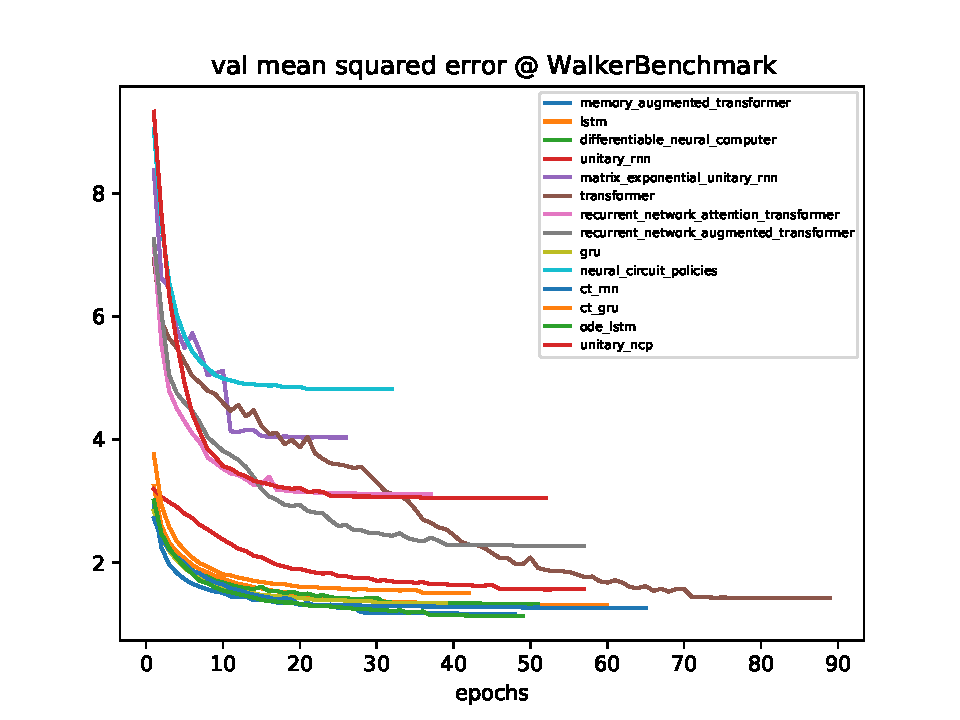
\includegraphics{../benchmark_logs/run_1/visualizations/#1/merged_visualizations.pdf}
        \caption{validation loss evolution during training for the #2 Benchmark on the second run}
        \label{fig:validation_loss_#1}
    \end{figure}
    \clearpage{}
}

\newcommand{\benchmarkplots}[2]{
    \subsection{#2 Benchmark}
    The training plots for the #2 Benchmark and each individual model will be shown on the following pages.
    \clearpage{}
    \begin{sidewaysfigure}[h]
        \centerline{
            \begin{minipage}[b]{0.5\linewidth}
                \centering
                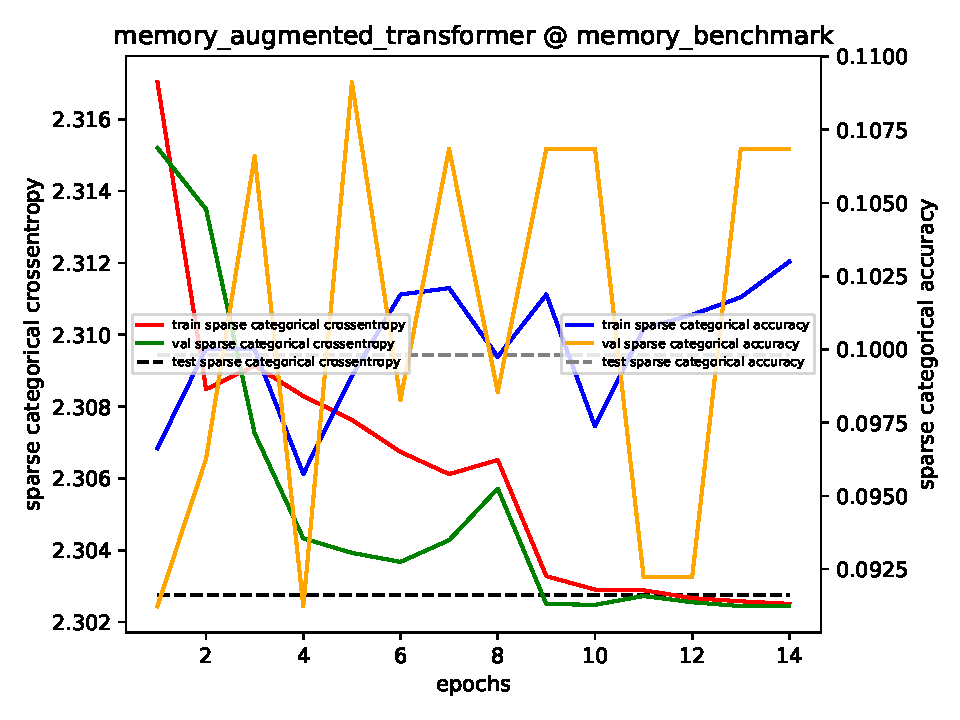
\includegraphics[width=\linewidth]{../benchmark_logs/run_1/visualizations/#1/memory_augmented_transformer.pdf}
            \end{minipage}
            \begin{minipage}[b]{0.5\linewidth}
                \centering
                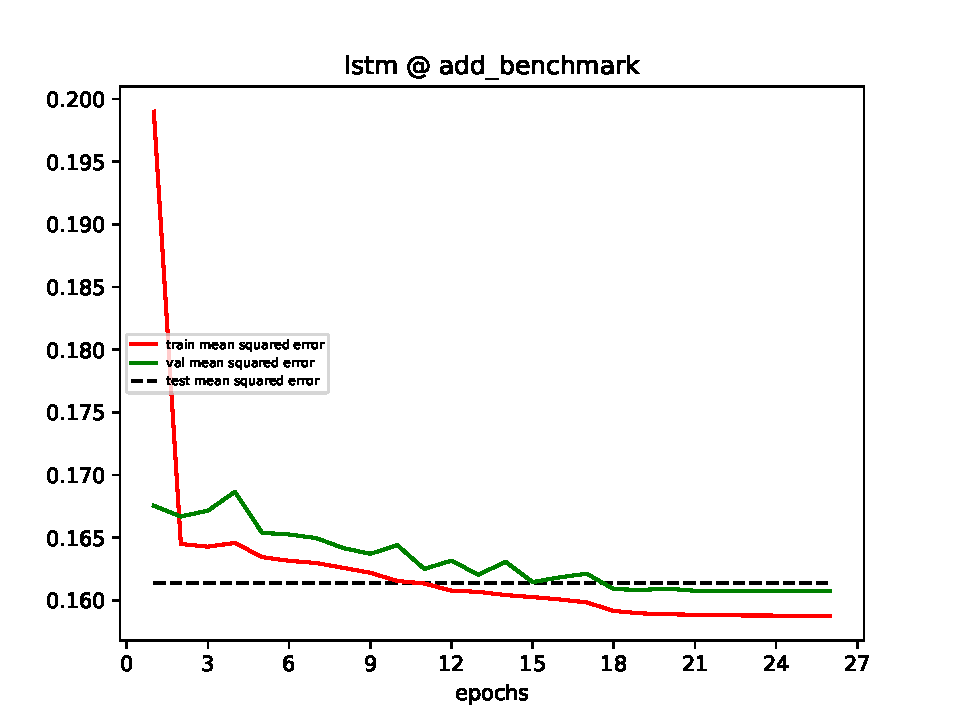
\includegraphics[width=\linewidth]{../benchmark_logs/run_1/visualizations/#1/lstm.pdf}
            \end{minipage}
        }
        \centerline{
            \begin{minipage}[b]{0.5\linewidth}
                \centering
                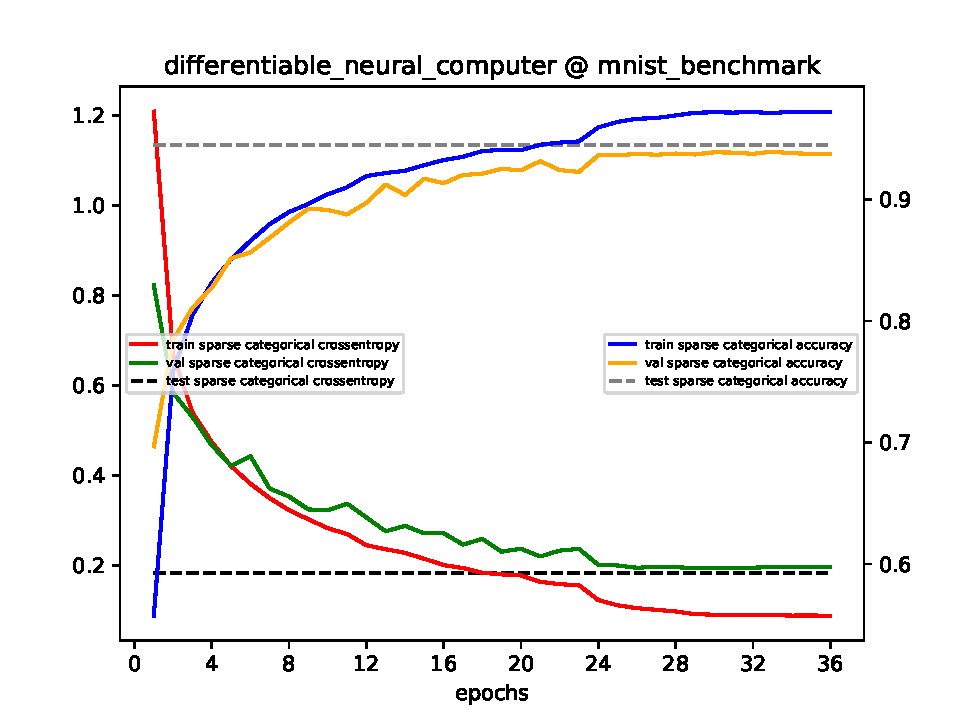
\includegraphics[width=\linewidth]{../benchmark_logs/run_1/visualizations/#1/differentiable_neural_computer.pdf}
            \end{minipage}
            \begin{minipage}[b]{0.5\linewidth}
                \centering
                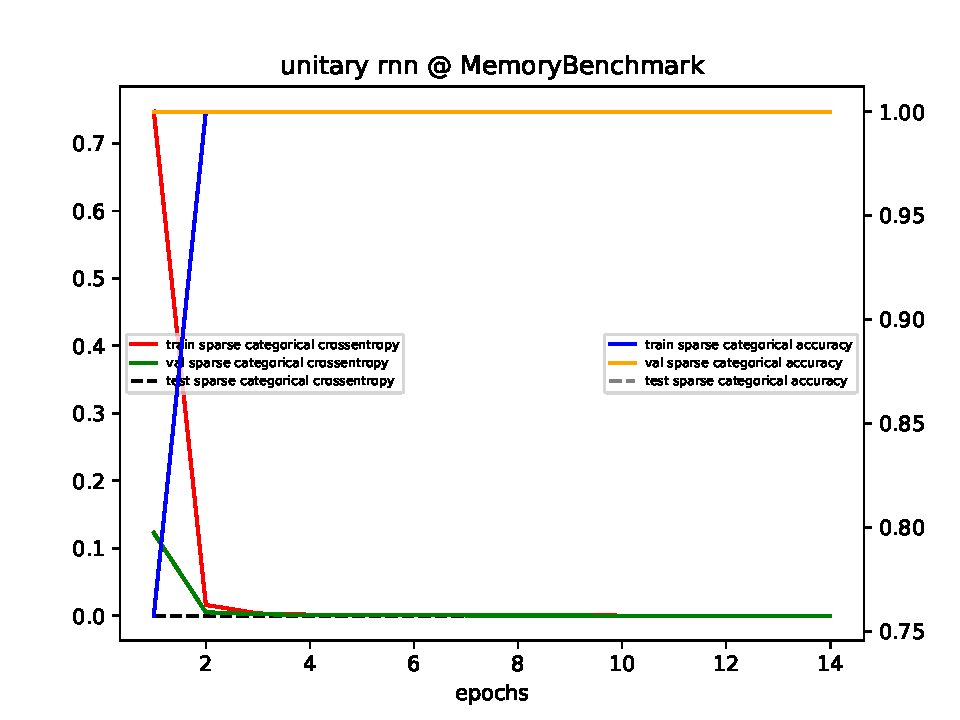
\includegraphics[width=\linewidth]{../benchmark_logs/run_1/visualizations/#1/unitary_rnn.pdf}
            \end{minipage}
        }
        \label{fig:#1_part_1}
        \caption{individual training plots for the #2 Benchmark on the second run - part 1}
    \end{sidewaysfigure}
    \begin{sidewaysfigure}[h]
        \centerline{
            \begin{minipage}[b]{0.5\linewidth}
                \centering
                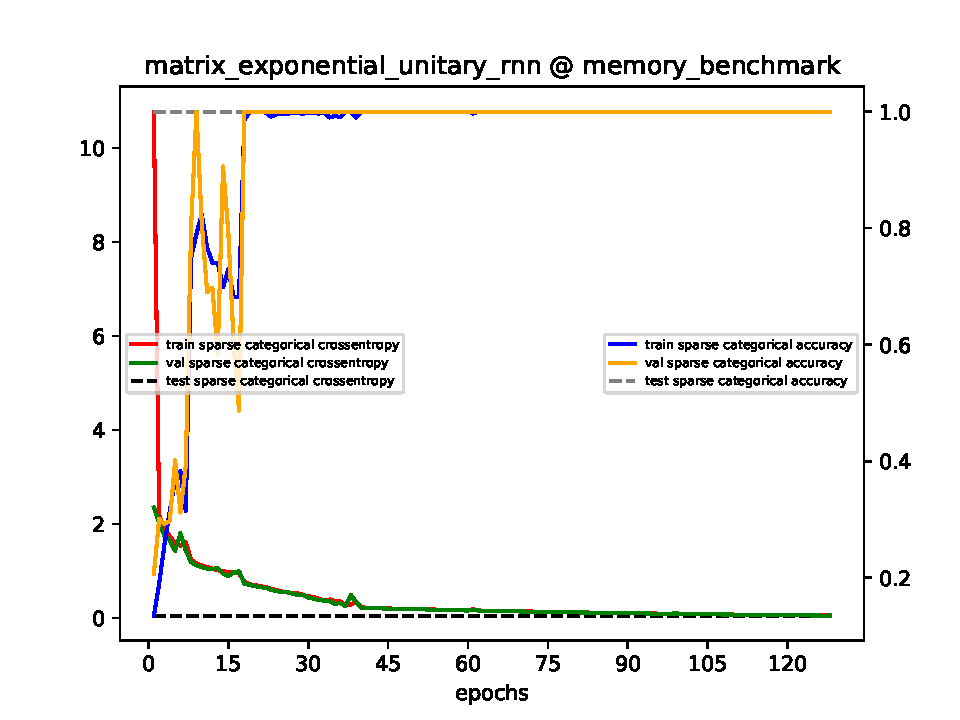
\includegraphics[width=\linewidth]{../benchmark_logs/run_1/visualizations/#1/matrix_exponential_unitary_rnn.pdf}
            \end{minipage}
            \begin{minipage}[b]{0.5\linewidth}
                \centering
                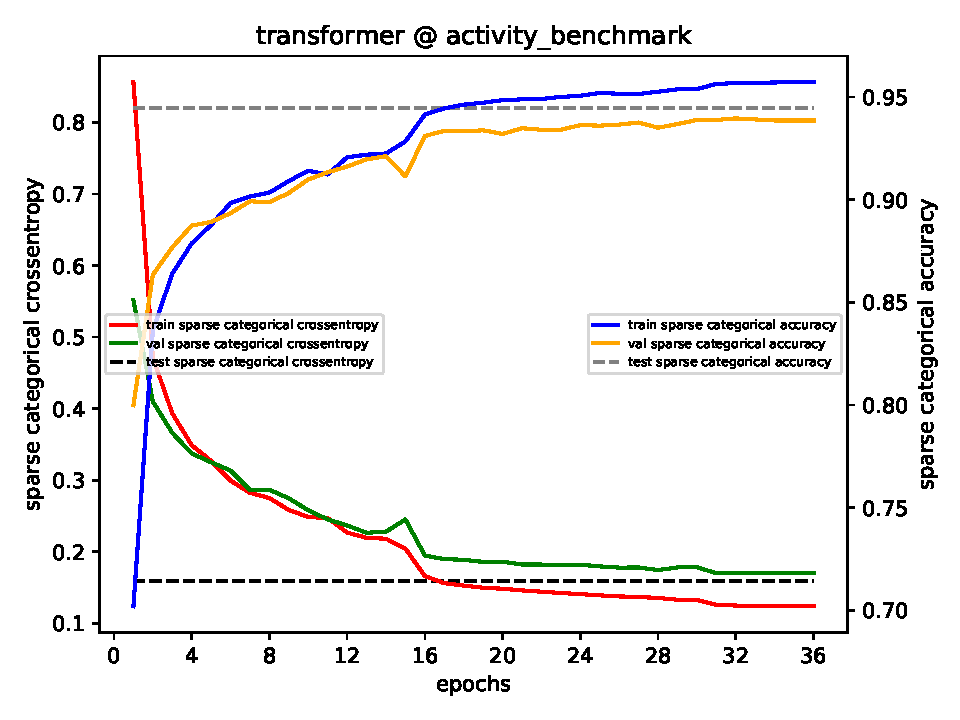
\includegraphics[width=\linewidth]{../benchmark_logs/run_1/visualizations/#1/transformer.pdf}
            \end{minipage}
        }
        \centerline{
            \begin{minipage}[b]{0.5\linewidth}
                \centering
                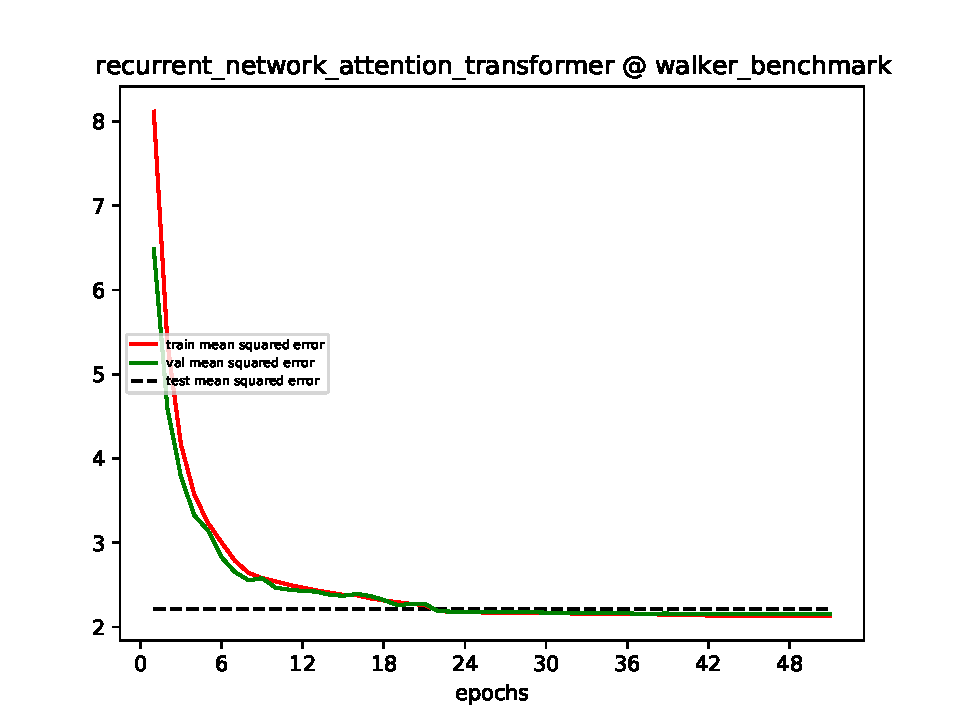
\includegraphics[width=\linewidth]{../benchmark_logs/run_1/visualizations/#1/recurrent_network_attention_transformer.pdf}
            \end{minipage}
            \begin{minipage}[b]{0.5\linewidth}
                \centering
                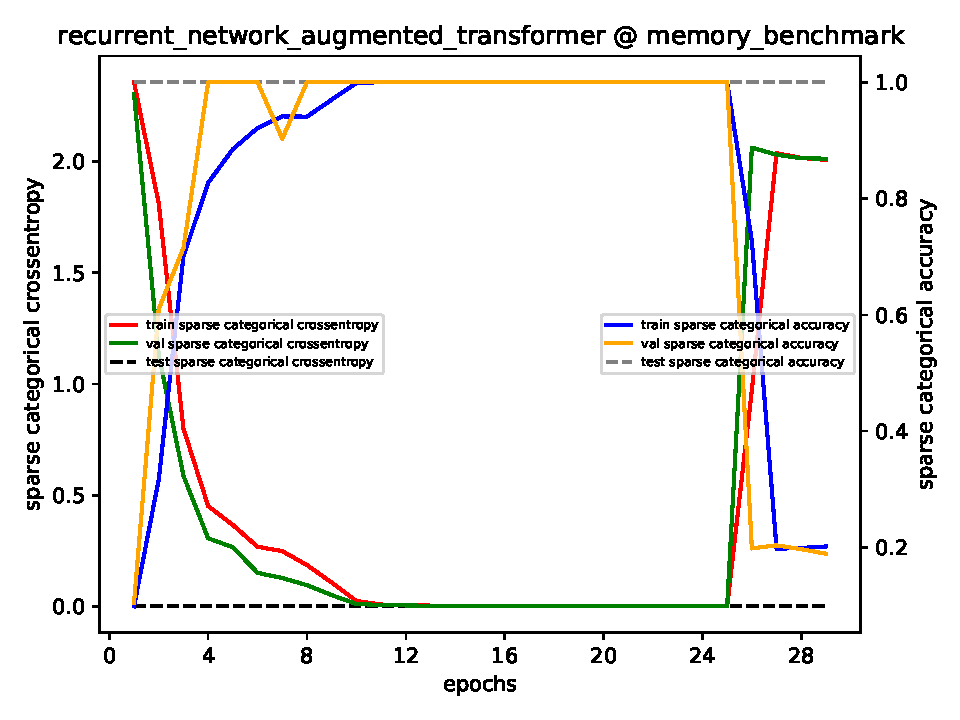
\includegraphics[width=\linewidth]{../benchmark_logs/run_1/visualizations/#1/recurrent_network_augmented_transformer.pdf}
            \end{minipage}
        }
        \label{fig:#1_part_2}
        \caption{individual training plots for the #2 Benchmark on the second run - part 2}
    \end{sidewaysfigure}
    \begin{sidewaysfigure}[h]
        \centerline{
            \begin{minipage}[b]{0.5\linewidth}
                \centering
                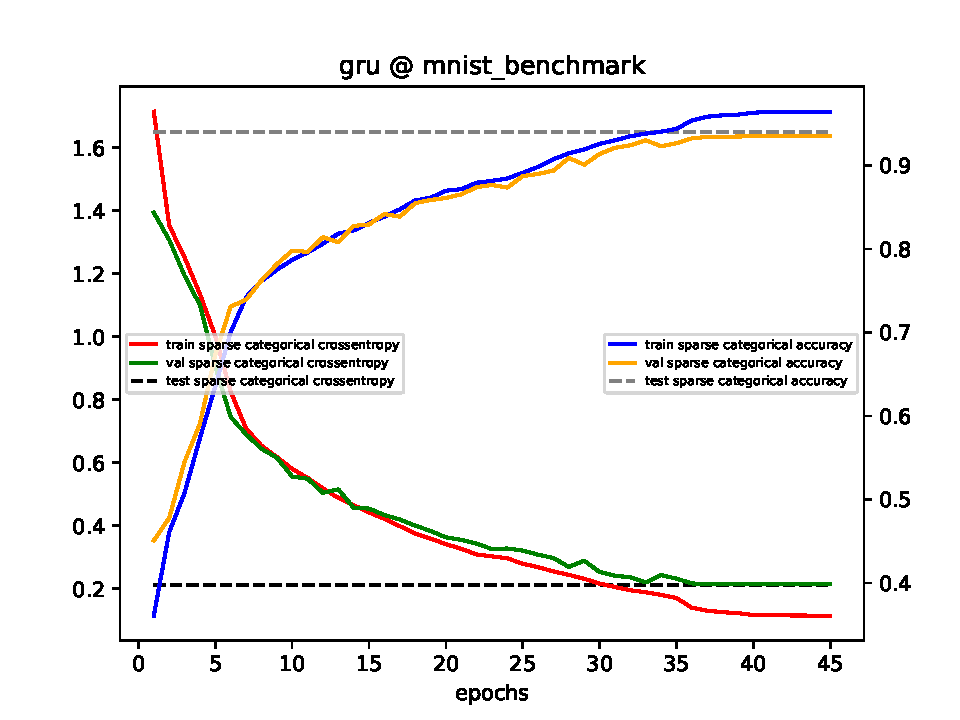
\includegraphics[width=\linewidth]{../benchmark_logs/run_1/visualizations/#1/gru.pdf}
            \end{minipage}
            \begin{minipage}[b]{0.5\linewidth}
                \centering
                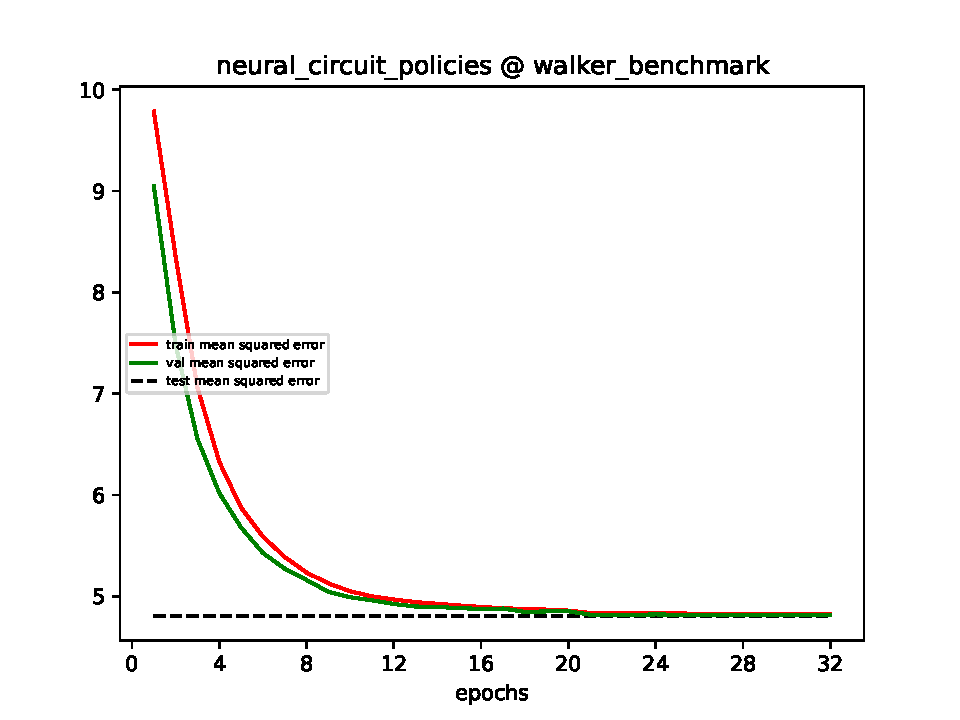
\includegraphics[width=\linewidth]{../benchmark_logs/run_1/visualizations/#1/neural_circuit_policies.pdf}
            \end{minipage}
        }
        \centerline{
            \begin{minipage}[b]{0.5\linewidth}
                \centering
                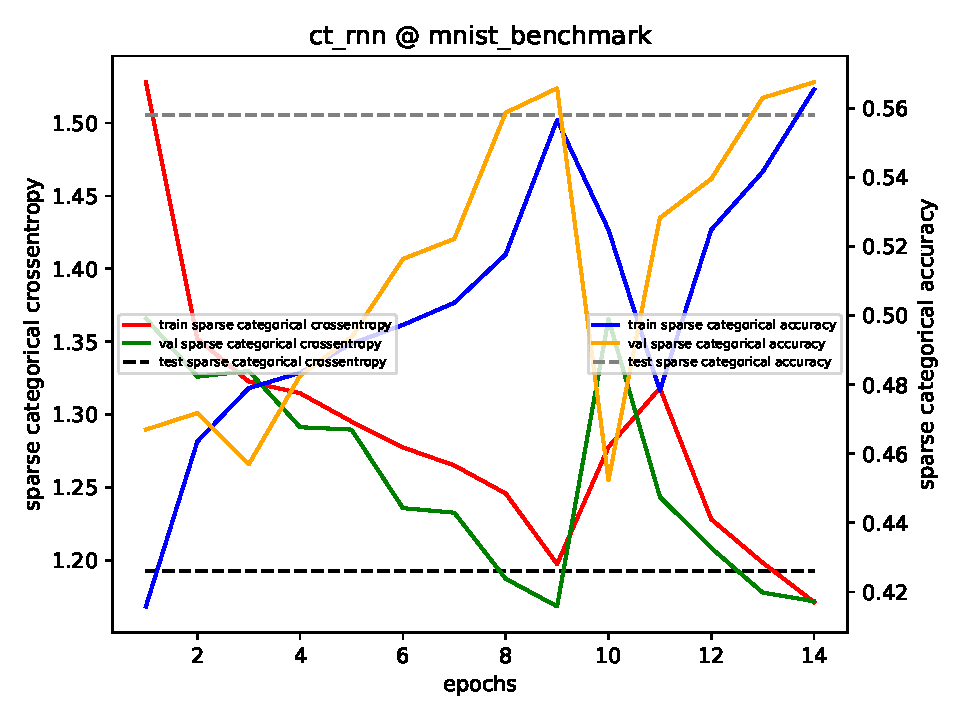
\includegraphics[width=\linewidth]{../benchmark_logs/run_1/visualizations/#1/ct_rnn.pdf}
            \end{minipage}
            \begin{minipage}[b]{0.5\linewidth}
                \centering
                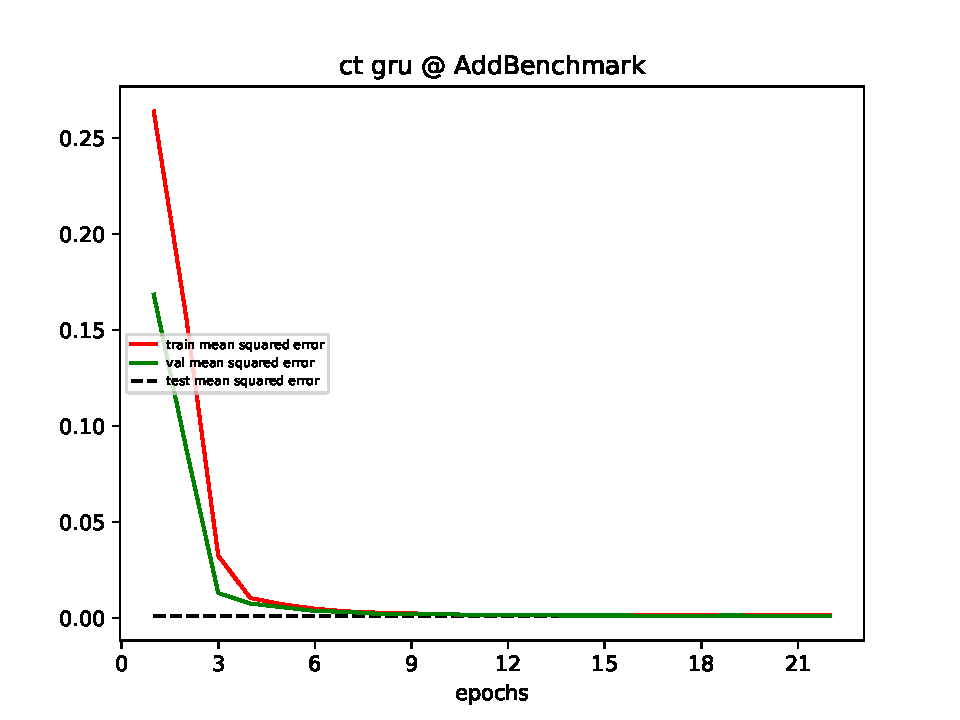
\includegraphics[width=\linewidth]{../benchmark_logs/run_1/visualizations/#1/ct_gru.pdf}
            \end{minipage}
        }
        \label{fig:#1_part_3}
        \caption{individual training plots for the #2 Benchmark on the second run - part 3}
    \end{sidewaysfigure}
    \begin{sidewaysfigure}[h]
        \centerline{
            \begin{minipage}[b]{0.5\linewidth}
                \centering
                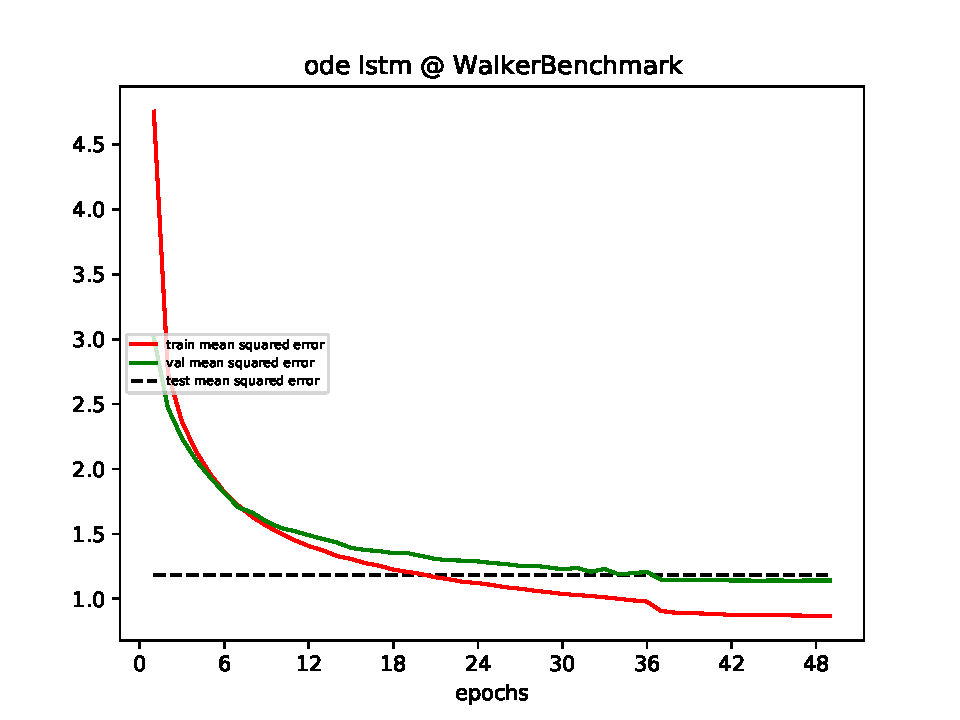
\includegraphics[width=\linewidth]{../benchmark_logs/run_1/visualizations/#1/ode_lstm.pdf}
            \end{minipage}
            \begin{minipage}[b]{0.5\linewidth}
                \centering
                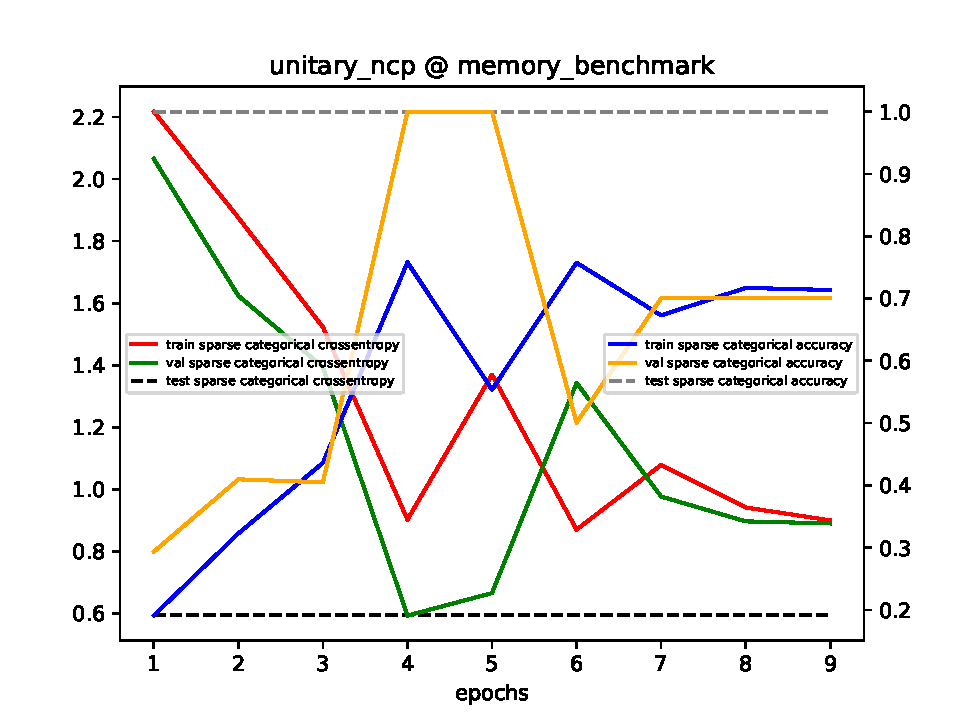
\includegraphics[width=\linewidth]{../benchmark_logs/run_1/visualizations/#1/unitary_ncp.pdf}
            \end{minipage}
        }
        \label{fig:#1_part_4}
        \caption{individual training plots for the #2 Benchmark on the second run - part 4}
    \end{sidewaysfigure}
    \clearpage{}
}

\begin{document}

    \frontmatter % Switches to Roman numbering.
% The structure of the thesis has to conform to the guidelines at
%  https://informatics.tuwien.ac.at/study-services

    \addtitlepage{naustrian} % German title page (not for dissertations at the PhD School).
    \addtitlepage{english} % English title page.

    \AddStatementPage

%\begin{danksagung*}
%\todo{Ihr Text here.}
%\end{danksagung*}

    \begin{acknowledgements*}
        d
        First, I have to thank Ramin for providing me excellent support throughout my work on the thesis.
        He cared about me and always pointed me to state-of-the-art literature, as he wanted to push me forward.
        I also have to thank Prof. Grosu for participating in numerous online meetings and sharing his in-depth knowledge in the machine learning domain.
        Furthermore, I want to thank Mathias Lechner for giving me first-class support on questions I had regarding various machine learning models.
        I have to expressly point out that he was always willing to help me and provided his responses incredibly fast.
        Finally, I have to thank my parents for providing me with mental and financial support throughout my whole study journey.
    \end{acknowledgements*}

    \begin{kurzfassung}
        Die Vielfalt der Modelle für maschinelles Lernen hat in den letzten Jahren mit dem Aufblühen der Forschung in diesem Bereich rapide zugenommen.
        Diese Arbeit versucht einen Überblick über Modelle zu geben, die in der Lage sind mit regelmäßig abgetasteten Zeitreihendaten umzugehen, ohne eine vorgegebene Historienlänge zu spezifizieren, die vom Modell berücksichtigt werden soll.
        Daher sind alle in dieser Arbeit vorgestellten Modelle entweder Abkömmlinge des rekurrenten neuronalen Netzes oder der Transformer-Architektur \cite{Transformer}.
        Darüber hinaus wurden neue Modelle eingeführt, um die gegebene Architektur des Transformers \cite{Transformer} und des unitären rekurrenten neuronalen Netzes \cite{EfficientUnitaryRNNs} zu verbessern.
        Nach der Einführung aller Modelle werden sie anhand fünf Benchmarks verglichen.
        Diese Benchmarks versuchen die Fähigkeit der Modelle zur Erfassung langfristiger Abhängigkeiten und die Fähigkeit der Modelle zur Modellierung physikalischer Systeme zu testen.
        Darüber hinaus wird eine zeitkontinuierliche Speicherzelle eingeführt, die in der Lage ist, ein Datenbit über eine große Anzahl von Zeitschritten zu speichern, ohne die gespeicherte Information zu verlieren.
        Diese Speicherzelle wird unter Verwendung der LTC-Network-Architektur \cite{LTCNetworks} aufgebaut.
        Der gesamte für diese Arbeit verwendete Code ist unter \url{https://github.com/Oidlichtnwoada/NeuralNetworkArena} verfügbar.
    \end{kurzfassung}

    \begin{abstract}
        The diversity of machine learning models has rapidly increased in recent years as research in the machine learning domain flourishes.
        This thesis tries to give an overview of machine learning models that are capable of dealing with regularly sampled time series data without specifying a given history length that should be taken into account by the model.
        Therefore, all models presented in this thesis are either derivatives of the recurrent neural network or the Transformer \cite{Transformer} architecture.
        Furthermore, new machine learning models have been introduced to improve the given Transformer \cite{Transformer} and unitary recurrent neural network \cite{EfficientUnitaryRNNs} architecture.
        After the introduction of all models, they are all benchmarked against five benchmarks and compared thoroughly.
        These benchmarks try to determine the model's capabilities to capture long-term dependencies and the ability to model physical systems.
        Moreover, the time-continuous Memory Cell architecture is introduced that is capable of storing a data bit over a large number of time steps without losing the stored information.
        This architecture is built using the LTC network \cite{LTCNetworks} architecture.
        All code used for this thesis is available under \url{https://github.com/Oidlichtnwoada/NeuralNetworkArena}.
    \end{abstract}

% Select the language of the thesis, e.g., english or naustrian.
    \selectlanguage{english}

% Add a table of contents (toc).
    \tableofcontents % Starred version, i.e., \tableofcontents*, removes the self-entry.

% Switch to Arabic numbering and start the enumeration of chapters in the table of content.
    \mainmatter


    \chapter{Introduction}

    A machine learning model is a mathematical parametrized function that gets input and produces an output.
    For example, the machine learning model GPT-3 proposed in \cite{GPT-3} has 175 billion scalar parameters.
    This thesis will use imitation learning to set the parameters of machine learning models optimally.
    Imitation learning means an associative expected output provided for each input that the model should return by applying its function to the input.
    Of course, when the model's function is applied to the input with the model's parameters' initial state, the returned model output will differ from the desired output in almost all cases.
    The measure responsible for quantifying this error between model output and the expected output is called a loss function and has a scalar return value.
    A sample loss function can be constructed quickly by computing the mean of all squared errors between the model output and the expected output.
    The model output is also often denoted as the prediction of the model.
    For each input sample, the loss function describes the error the model makes by applying its function, and this error is only dependent on the model's parameters.
    In practice, the loss function is applied to a batch of inputs separately, and the arithmetic mean of all scalar loss function return values of the individual input samples is used as a loss function to differentiate.
    The size of this input batch is called batch size.
    A computer scientist wants to find the global minimum of that function concerning all machine learning model parameters in the general case.
    A visualized loss surface where the loss function return value is plotted in the z-axis and all possible model parameter combinations are given as points on the plane is given as follows:
    \begin{figure}[H]
        \centering{}
        \includegraphics[page=1,width=0.8\linewidth,trim={105 107 305 510},clip]{literature/visualizing_the_loss_landscape_of_neural_nets.pdf}
        \caption{visualized loss surface \cite[p. 1]{loss_vis}}
        \label{fig:loss_vis}
    \end{figure}
    As this is a problem that cannot be solved analytically in most cases, it is approximated by using gradient descent \cite[p. 6-12]{GradientDescent}.
    This method incrementally changes each parameter depending on the gradient of each parameter's loss function in a lockstep fashion.
    By denoting the loss function with $L$, the learning rate with $\alpha$, the whole old parameter set with $p$, the old single scalar parameter with $p_i$ and the new single scalar parameter with $p_i'$, the formula to update the individual parameters $p_i$ in a single gradient descent step can be given as follows \cite[p. 6-12]{GradientDescent}:
    \begin{align}
        \label{gradient_descent_update}
        \forall p_i:~p_i' &= p_i - \alpha * \frac{\partial{L}}{\partial{p_i}}(p)
    \end{align}
    It is essential to note that the model and the loss measure must be deterministic functions for the gradient to exist.
    This update rule ensures that if the loss function increases with increasing $p_i$, a decrease of the parameter will happen, leading to a decreasing loss function result.
    The opposite case holds as well, which is why there is a minus sign in \Cref{gradient_descent_update}.
    The learning rate $\alpha$ determines how significant in magnitude the update to the parameters should be at each gradient descent step.
    A too-small learning rate will lead to slow convergence, and a too-large learning rate will lead to divergence.
    Therefore, a too-large learning rate is far more dangerous than a too-small one.
    Convergence means that the parameter updates have led to a local minimum of the loss function.
    There are no guarantees that this is the global minimum. Divergence means that the loss function diverges towards infinity.
    A local minimum or convergence can be reached by applying the gradient descent update rule to as many inputs as needed to set the loss function derivative to nearly zero.
    The trajectory of the parameter set on the loss surface when repeatedly applying the gradient descent update rule was visualized in \cite[p. 2]{gradient_descent_vis} with the initial starting parameter set denoted as a black triangle as follows:
    \begin{figure}[H]
        \centering{}
        \includegraphics[page=2,width=0.8\linewidth,trim={90 585 355 75},clip]{literature/gradvis_visualization_and_second_order_analysis_of_optimization_surfaces_during_the_training_of_deep_neural_networks.pdf}
        \caption{visualization of gradient descent}
        \label{fig:gradient_descent_vis}
    \end{figure}
    The differentiation of the loss function, which can be represented as a computational graph with lots of nested functions, involves many chain rule applications for the individual model parameter derivatives. The machine learning term for repeatedly applying the chain rule is backpropagation.
    If these nested functions correspond to applying the same machine learning model function across multiple input time steps as done in recurrent neural networks, then this backpropagation procedure can also be called backpropagation through time as introduced in \cite[p. 6-12]{GradientDescent}.
    The chain rule for differentiating $z(y(x_0))$ with respect to $x$ for $x=x_0$ where $z$ and $y$ are both functions in a single variable is given by:
    \begin{align}
        \label{chain_rule}
        \frac{dz}{dx} \Bigr\rvert_{x=x_0} = \frac{dz}{dy} \Bigr\rvert_{y=y(x_0)} * \frac{dy}{dx} \Bigr\rvert_{x=x_0}
    \end{align}
    The above equation reveals that a machine learning framework has to compute all partial derivatives of all functions present in the above-mentioned computational graph.
    Furthermore, it must keep track of the so-called activations, which are denoted by $y(x_0)$ in the above \Cref{chain_rule}, as otherwise the gradient of the loss function with respect to the individual parameters cannot be computed.
    As this can use lots of memory, reversible layers were introduced by \cite{ReversibleLayer} where intermediate activations can be computed from the layer's output vector, which makes storing intermediate activations obsolete.


    \section{Problem Statement}
    As the sheer amount of different machine learning models can be overwhelming, the task was to fix a distinct application domain and compare the most influential machine learning models in this domain with suitable benchmarks.
    Benchmarks are just large input data sets with associative expected outputs.
    Additionally, ideas for possible improvements in existing architectures should be implemented and benchmarked against existing ones.
    All benchmarked models should be implemented in the same machine learning framework, and the benchmark suite should be extensible and reusable for other machine learning research projects.
    The whole implementation work done for this thesis should be accessible for everyone by open-sourcing all the code.
    As mentioned in the abstract, all the models covered in this thesis are either derivatives of the recurrent neural network or the Transformer \cite{Transformer} architecture.
    The benchmarks used in this thesis either test the models for their capabilities to capture long-term dependencies or their ability to model physical systems.


    \section{How to better model Physical Systems} \label{physical_systems}
    Differential equations guide physical systems. The relation between system state $x$, system input $u$ and system output $y$ is given by the state derivative function $f$ and the output function $h$, both of which depend on the absolute time $t$, as follows:
    \begin{align}
        \label{physical_system_equations_state}
        \dot x(t) &= f(x(t),u(t),t) \\
        \label{physical_system_equations_output}
        y(t) &= h(x(t),u(t),t)
    \end{align}
    This form of system description applies to all continuous physical systems in our daily surroundings. Most of these systems are even time-invariant.
    This means the functions $f$ and $h$ do not depend on the absolute time $t$.
    For example, a mechanical pendulum will now approximately behave the same as in one year, as its dynamics do not depend on the absolute time $t$.
    The system description presented in \Cref{physical_system_equations_state} and \Cref{physical_system_equations_output} proposes that machine learning models built similarly and whose state is also determined by a differential equation should be pretty capable of modeling the input-output relation of physical systems.
    When the benchmarked models are introduced in more detail, it can be seen that all continuous-time machine learning models use a comparable structure in terms of parameterizing the state derivative and the output function.
    The key takeaway point is that continuous physical systems map an input function $x(t)$ to an output function $y(t)$ as visualized in \cite[p. 102]{dsp}:
    \begin{figure}[H]
        \centering{}
        \includegraphics[page=102,width=0.8\linewidth,trim={110 580 140 60},clip]{literature/digital_signal_processing.pdf}
        \caption{visualization of input-output relation of a continuous system}
        \label{fig:continuous_system_vis}
    \end{figure}


    \section{Sampled Physical Systems} \label{sampled_physical_systems}
    As the current state's evaluation $x$ at time point $t'$, with initial state $x_0$ given the dynamics from \Cref{physical_systems}, can be computationally very expensive even infeasible, sampling was introduced to avoid solving a complex differential equation.
    Therefore, the whole system is only observed at equidistant successive time instants, values belonging to this time instant are denoted with a subscript index $k \in \mathbb{Z}$, and the system is now called discrete.
    Difference equations guide discrete systems. The relation between system state $x$, system input $u$ and system output $y$ is given by the next state function $f$ and the output function $h$, both of which depend on the time instant $k$, as follows:
    \begin{align}
        \label{discrete_system_equations_state}
        x_{k+1} &= f(x_k,u_k,k) \\
        \label{discrete_system_equations_output}
        y_k &= h(x_k,u_k,k)
    \end{align}
    It must be noted that $x$ and $y$ are time series in discrete systems and no more functions like in continuous-time physical systems.
    This slightly off-topic explanation is necessary, as vanilla recurrent neural networks are built using the same principle.
    The system equations, \Cref{discrete_system_equations_state} and \Cref{discrete_system_equations_output}, require a regularly (equidistantly) sampled input $x$.
    A similar argument as before in \Cref{physical_systems} proposes now that a machine learning model with a similar structure, which gets a regularly sampled input of a physical system, should also be pretty capable of modeling the input-output relation of this sampled physical system.
    The corresponding machine learning models are then called discrete-time machine learning models.
    The key takeaway point is that discrete physical systems map an input sequence $x[n]$ to an output sequence $y[t]$ as visualized in \cite[p. 102]{dsp}:
    \begin{figure}[H]
        \centering{}
        \includegraphics[page=102,width=0.8\linewidth,trim={110 485 140 150},clip]{literature/digital_signal_processing.pdf}
        \caption{visualization of input-output relation of a discrete system}
        \label{fig:discrete_system_vis}
    \end{figure}


    \section{Why capturing Long-Term Dependencies is difficult} \label{long_term_difficult}
    The difficulty will be outlined solely on the example of vanilla recurrent neural networks (RNNs).
    How Transformer-based and advanced RNN architectures tackle the problem will be discussed later.
    Vanilla recurrent neural networks are discrete-time machine learning models.
    Its dynamics are similar to the equations that govern sampled physical systems in \Cref{sampled_physical_systems}.
    The current state vector $h_{t}$ and the next input vector $x_{t+1}$ determine the next state vector $h_{t+1}$ and output vector $y_{t+1}$ deterministically.
    In this model, all the past inputs are implicitly encoded in the current state vector.
    This implicit encoding entails a big challenge for computer scientists, as computers only allow states of finite size and finite precision, unlike our physical environment, which results in an information bottleneck in the state vector.
    The next state of a vanilla recurrent neural network $h_{t+1}$ and its output $y_{t}$ is typically computed by equations like the two proposed in \cite[p. 2]{UnitaryRNNs} by using a non-linear bias-parametrized activation function $\sigma$, three matrices ($W$, $V$ and $U$) and the output bias vector $b_o$:
    \begin{align}
        \label{rnn_state_update}
        h_{t+1} &= \sigma(W*h_t + V*x_{t+1}) \\
        \label{rnn_output}
        y_{t} &= U*h_{t} + b_o
    \end{align}
    Without the time shift on the input in the next state equation given in \Cref{rnn_state_update}, the equations are similar to those describing sampled physical systems.
    \Cref{rnn_state_update} can be visualized by the following figure:
    \begin{figure}[H]
        \centering{}
        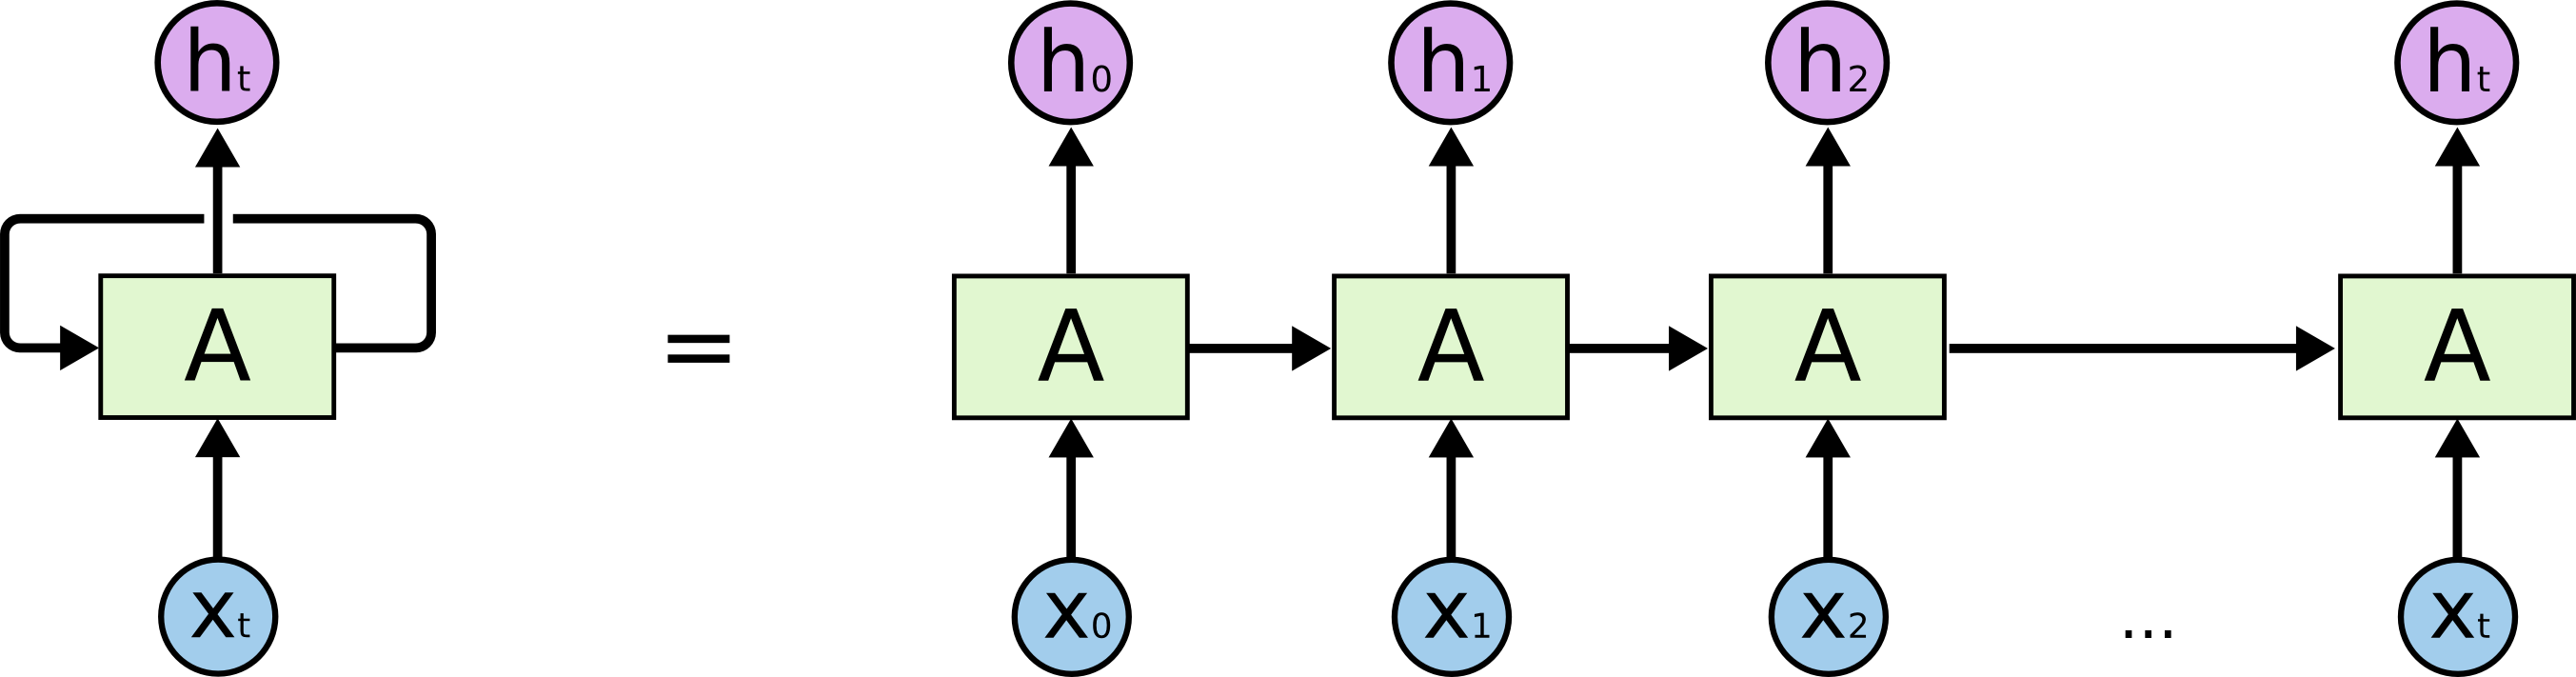
\includegraphics[width=0.8\linewidth]{graphics/rnn.png}
        \caption{visualization of an RNN state update \cite{rnn_vis}}
        \label{fig:rnn_vis}
    \end{figure}
    The following inequality from \cite[p. 2]{UnitaryRNNs} using norms shows the relation between the loss derivative, a recent state $h_T$ and a state from the distant past $h_t$ where $T \gg t$.
    The notation is kept similar to the examples before. A subscript $2$ after a vector norm denotes the Euclidean norm, and a subscript $2,ind$ after a matrix norm denotes the spectral norm:
    \begin{align}
        \label{gradient_formula}
        \left\Vert \pdv{L}{h_t} \right\Vert_2 \leq \left\Vert \pdv{L}{h_T} \right\Vert_2 * \left\Vert W \right\Vert_{2,ind}^T * \prod^{T-1}_{k=t} \left\Vert diag(\sigma'(W*h_k + V*x_{k+1})) \right\Vert_{2,ind}
    \end{align}
    This inequality contains all essential parts to understand why capturing long-term dependencies with vanilla recurrent neural networks is difficult.
    Some problems that machine learning tries to solve require incorporating input data from the distant past to make good predictions in the present.
    As these inputs are implicitly encoded in the states of the distant past, $\left\Vert \pdv{L}{h_t} \right\Vert_2$ should not decay to zero or grow unboundedly to effectively tune the parameters using the gradient descent update rule shown above in \Cref{gradient_descent_update}.
    This persistence of the gradient ensures that distant past inputs influence the loss function reasonably and makes it feasible to incorporate the knowledge to minimize the loss function.
    As known, the spectral norm of the diagonal matrix in \Cref{gradient_formula} is just the largest magnitude out of all diagonal entries.
    Therefore, if the diagonal matrix's norm is close to zero over multiple time steps $k$, the desired loss gradient will decay towards zero.
    Otherwise, if the diagonal matrix's norm is much larger than one over multiple time steps $k$, the desired loss gradient may grow unboundedly.
    Using this knowledge, it is now clear that a suitable activation function must have a derivative of one in almost all cases to counteract the above-described problems.
    A good fit would be a rectified linear unit (relu) activation function with an added bias term.
    The relu activation function with a bias $b$ can simply be discribed by the function $max(0,x+b)$. The $max$ function should be applied element-wise.
    As the requirements for the activation function candidates are precisely formulated now, the next thing to discuss is the norm of the matrix $W$.
    If $\left\Vert W \right\Vert_{2,ind} > 1$, $\left\Vert \pdv{L}{h_t} \right\Vert$ may grow unboundedly, making it difficult to apply the gradient descent technique to optimize parameters.
    If $\left\Vert W \right\Vert_{2,ind} < 1$, $\left\Vert \pdv{L}{h_t} \right\Vert$ will decay to $0$, making it impossible to apply the gradient descent technique to optimize parameters.
    These problems are identical to the norm of the diagonal matrix and have the same implications.
    The first case is called the exploding gradient problem, and the second case is called the vanishing gradient problem for given reasons.
    Both phenomena are explained in more detail in \cite{LongTermDependenciesGradientDescent}.


    \section{Objectives and Main Motivations}
    This work objectively compares various machine learning models used to process regularly sampled time series data.
    It should outline the weaknesses and strengths of the benchmarked models and determine their primary domain of use.
    Moreover, as there are many models benchmarked, their relative expressivity across various application domains can be compared reasonably well.
    Another aim is to provide an overview of what architectures are currently available and how they can be implemented.
    Furthermore, the implemented benchmark suite should be reusable for future projects in the machine learning domain.


    \section{Methodological Approach}
    The first part of this thesis was to determine the most influential models for processing time series data.
    Some models that were benchmarked against each other in this thesis were taken from \cite{ODELSTM}, even though this paper focuses primarily on irregularly sampled time series.
    The other models were implemented according to the following architectures: Long Short-Term Memory \cite{LSTM}, Differentiable Neural Computer \cite{DNC}, Unitary Recurrent Neural Network \cite{EfficientUnitaryRNNs}, Transformer \cite{Transformer} and Neural Circuit Policies \cite{NCP}.
    These nine models are then complemented by five models that were newly introduced.
    All these models are benchmarked against each other.
    Additionally, the time-continuous Memory Cell architecture should be introduced.
    This architecture must have a dedicated benchmark test and should not be benchmarked against all other fully-fledged machine learning models as it is only a proof-of-concept implementation.
    All mentioned models should be implemented in the machine learning framework Tensorflow \cite{Tensorflow}.
    After implementing all models, an extensible benchmark suite had to be implemented to compare all implemented models.
    A basic benchmark framework should be implemented, which automatically trains a given model and saves all relevant information regarding the training process, including generating plots to visualize the data.
    All that should be needed to implement a new benchmark is to specify the input, the expected output data, the loss function, and the model's required output vector size.
    The benchmarks regarding person activity classification, sequential MNIST classification, and kinematic physics simulation were taken from \cite{ODELSTM} and were modified slightly to be compatible with the benchmark framework.
    The other two benchmarks regarding the copying memory and the adding problem were taken from \cite{UnitaryRNNs} but were also slightly modified to fit the benchmark framework's needs.
    The sixth benchmark that had to be implemented was the Cell Benchmark that should check if the Memory Cell can store information over many time steps.
    When this step is also done, all benchmarks should be run on all applicable models, and then the results should be thoroughly compared to filter out the strengths and weaknesses of the diverse models.
    Only after that, a summary should be written to concisely summarize the most important discoveries and fallacies that were made.


    \section{State of the Art}
    The whole field of sequence modeling started with recurrent neural networks.
    More and more modern machine learning architectures exploit the fact that continuous-time models are very well suited for tasks related to dynamical physical systems as explained in \Cref{physical_systems}.
    A few examples for such models would be the CT-GRU \cite{CTGRU}, the LTC network \cite{LTCNetworks} and the ODE-LSTM architecture \cite{ODELSTM}.
    Nevertheless, some older architectures exploit continuous-time dynamics in machine learning models like the CT-RNN architecture \cite{CTRNN}.
    The other problem described in the previous chapters is the challenging task of capturing long-term dependencies in time series.
    One solution for the problem was proposed in \cite{UnitaryRNNs}, which introduced the Unitary RNN architecture.
    In principle, this architecture uses the vanilla RNN architecture described above. The difference is that the matrix $W$ fulfills $\left\Vert W \right\Vert_{2,ind} = 1$ to tackle the vanishing and exploding gradient problem.
    This idea was later refined by \cite{EfficientUnitaryRNNs}.
    The vanishing gradient problem was also tackled by the LSTM architecture \cite{LSTM} using a gating mechanism.
    This mechanism changes the subsequent state computation of the vanilla RNN.
    Another possible mitigation to the vanishing gradient problem is the transformer architecture proposed in \cite{Transformer} using a mechanism called attention.
    In principle, the Transformer architecture model has access to all past inputs simultaneously and directs its attention to the inputs most relevant for solving the required task.
    This global access eliminates the need to backpropagate the error through multiple time-steps, which keeps the number of backpropagation steps low.

%\todo{Enter your text here.}


    \chapter{Models}
    In this chapter all benchmarked models are introduced and theoretically discussed.
    At first, \Cref{model_factory} describes how the models with the correct output vector size used in the benchmark framework introduced in \Cref{benchmark_framework} are constructed.
    Then machine learning models that use a gating mechanism to capture long-term dependencies are introduced.
    These are the LSTM introduced in \Cref{lstm}, the ODE-LSTM introduced in \Cref{odelstm}, the GRU introduced in \Cref{gru} and the CT-GRU introduced in \Cref{ctgru}.
    Furthermore, three continuous-time models (the Neural Circuit Policies, the CT-RNN and the Memory Cell) are introduced in \Cref{ncp}, \Cref{ctrnn} and \Cref{memory_cell}.
    Moreover, two discrete-time architectures with bounded loss gradients are introduced which are given as the Unitary RNN introduced in \Cref{urnn} and the Matrix Exponential Unitary RNN introduced in \Cref{meurnn}.
    In \Cref{transformer} the Transformer architecture is introduced which has an encoder-decoder structure and uses an attention mechanism to capture long-term dependencies.
    The two MANN (memory-augmented neural network) architectures given as the Memory Augmented Transformer and the Differentiable Neural Computer are introduced in \Cref{mat} and \Cref{dnc}.
    Three architectures (the Unitary NCP, the Recurrent Network Augmented Transformer and the Recurrent Network Attention Transformer) mix approaches from other models and try to combine their advantages.
    These models are elaborated in \Cref{uncp}, \Cref{rnaut} and \Cref{rnatt}.


    \section{Model Factory} \label{model_factory}
    As all the benchmarks require variants of the same models with different output vector sizes, a model factory function was implemented to produce an output tensor given the model's name, the output vector size, and the input tensor tuple.
    This function was called \texttt{get\_model\_output\_by\_name} and can be found under \url{https://github.com/Oidlichtnwoada/NeuralNetworkArena/blob/master/experiments/models/model_factory.py}.
    This mechanism of creating the output tensor, including the internal computational graph of the Tensorflow library \cite{Tensorflow} is called the Functional API.
    Most of the models were parameterized such that they have roughly $20000$ trainable parameters in the Walker Benchmark described in \Cref{walker} as this benchmark features the largest input and output vector size of all benchmarks.
    The exceptions of the parameter count are the Unitary RNN model given in \Cref{urnn}, the NCP model given in \Cref{ncp}, the Unitary NCP model given in \Cref{uncp}, the Recurrent Network Augmented Transformer given in \Cref{rnaut} and the Recurrent Network Attention Transformer given in \Cref{rnatt}.
    All these models' computational graphs lead to high computation costs during backpropagation, which leads to training durations up to a whole day for a single benchmark.
    This high computational cost was unacceptable, and therefore their parameter count was reduced to present at least some results for these models.


    \section{LSTM} \label{lstm}
    The LSTM (Long Short-Term Memory) recurrent neural network architecture is a discrete-time machine learning model introduced in \Cref{sampled_physical_systems}.
    The model has an ordinary (hidden) state vector and a cell state vector, which should store information over a longer time horizon than the hidden state vector.
    This thesis uses the open-source LSTM implementation provided by the Keras library \cite{Keras} which is based on the original LSTM paper \cite{LSTM} as well on its successor paper \cite{LSTM_forget} that introduces a forget mechanism for the LSTM.
    The function the LSTM model is applying to its inputs to produce the outputs is given as follows with inputs denoted as $x_t$ and outputs which equals the hidden states denoted as $h_t$ \cite[p. 4-8]{LSTM_forget}:
    \begin{align}
        \label{forget_gate} f_t &= sigmoid(W_f*x_t + U_f*h_{t-1} + b_f) \\
        \label{input_gate} i_t &= sigmoid(W_i*x_t + U_i*h_{t-1} + b_i) \\
        \label{output_gate} o_t &= sigmoid(W_o*x_t + U_o*h_{t-1} + b_o) \\
        \label{cell_input} \tilde{c}_t &= tanh(W_c*x_t + U_c*h_{t-1} + b_c) \\
        \label{cell_state} c_t &= f_t * c_{t-1} + i_t * \tilde{c}_t \\
        \label{hidden_state} h_t &= o_t * tanh(c_t)
    \end{align}
    The term $f_t$ in \Cref{forget_gate} is the forget gate's activation vector, $i_t$ in \Cref{input_gate} is the input gate's activation vector, $o_t$ in \Cref{output_gate} is the output gate's activation vector, $\tilde{c}_t$ in \Cref{cell_input} is the cell input activation vector, $c_t$ in \Cref{cell_state} is the cell state vector and $h_t$ in \Cref{hidden_state} is the hidden state vector or also called output vector of the LSTM model.
    The initial hidden state $h_0$ and the initial cell state $c_0$ are picked to the all-zero vector.
    Matrices are denoted with capital letters, and vectors are denoted with lower case letters.
    The LSTM model has a configurable state size. The multiplication sign between two vectors denotes a scalar product, and it denotes matrix multiplication between matrices and vectors.
    This convention is used throughout this thesis.
    Dimensions of matrices are picked such that the resulting vector has the required state size, which is configurable.
    The bias vectors denoted with $b$ also have the required state dimension.
    The matrices denoted by $W$ map the input vector in each time step and the matrices denoted by $U$ map the hidden state vector at each time step to a resulting vector.
    This architecture was also visualized in the successor paper as follows:
    \begin{figure}[H]
        \centering{}
        \includegraphics[page=6,width=0.8\linewidth,trim={175 535 200 55},clip]{literature/learning_to_forget_continual_prediction_with_lstm.pdf}
        \caption{visualized LSTM architecture \cite[p. 6]{LSTM_forget}}
        \label{fig:lstm_vis}
    \end{figure}
    The model structure allows it to capture long-term dependencies by setting $f_t$ equal to one and $i_t$ equal to zero in some common vector indices $i$, and only the previous cell state is used to build the next cell state in these following cell state vector entries.
    This will lead to $\frac{\partial{c_{t,i}}}{\partial{c_{t-1,i}}} = 1$, as this clearly approximates the identity function for a specific index $i$ in the cell state vector.
    Backpropagation to activations in the distant past is feasible using this model function as gradients are not vanishing or exploding when the model's parameters are correctly learned.
    This mechanism is called the constant error carrousel described in \cite[p. 7]{LSTM}.
    LSTMs can incorporate this mechanism to store essential information from the distant past, making accurate predictions when long-term dependencies are present.
    Furthermore, the model can also decide to forget the previous cell state entirely if the current input vector makes the stored cell state obsolete in the corresponding application.
    This forgetting is done by learning to set the forget gate's activation vector close to zero, and the cell input activation vector is then used to fill the cell state again if the input gate's activation vector is set accordingly.
    The output gate's activation vector determines which portion of the cell state is used to build the hidden state or output vector of the LSTM model.
    Throughout the thesis, an LSTM model with a fixed state vector size of $64$ was used. As mentioned in the benchmark framework section, each model must support an arbitrary output vector size.
    The correct model output vector size is accomplished by postprocessing the hidden state outputs of the LSTM by a dense layer with the required amount of output neurons and without an activation function.
    The output $y$ of a dense layer without an activation function and input vector $x$ can simply be given by: $y = W*x + b$.
    In this notation, $W$ is a matrix such that it maps the input vector $x$ to the required output size, and $b$ is just a bias vector as in the functions describing the LSTM model.
    The following figure visualizes three dense layers with parameters denotes as arrows:
    \begin{figure}[H]
        \centering{}
        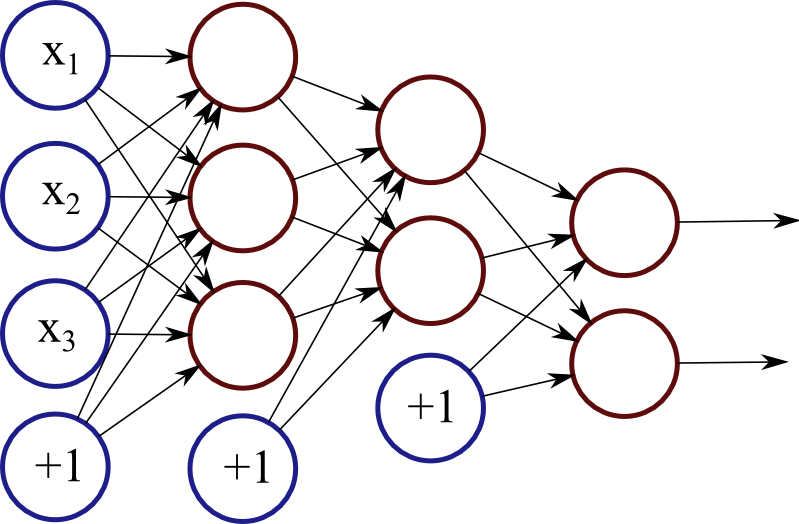
\includegraphics[width=0.5\linewidth]{graphics/dense.png}
        \caption{visualized dense layers \cite{dense_vis}}
        \label{fig:dense_vis}
    \end{figure}
    Training the LSTM model from the Keras library is fast as it uses an optimized cuDNN \cite{cuDNN} implementation.
    The LSTM model implementation used in this thesis is exposed under the \texttt{get\_lstm\_output} function defined in the file \url{https://github.com/Oidlichtnwoada/NeuralNetworkArena/blob/master/experiments/models/model_factory.py}.


    \section{GRU} \label{gru}
    The GRU (Gated Recurrent Unit) recurrent neural network architecture is a discrete-time machine learning model introduced in \Cref{sampled_physical_systems}.
    The model has only a single ordinary hidden state vector.
    This thesis uses the open-source GRU implementation provided by the Keras library \cite{Keras} which is based on the original GRU paper \cite{GRU}.
    The GRU model tries to simplify the LSTM architecture by removing the output gate, for example, without sacrificing expressivity.
    This simplification leads to a smaller parameter count of a GRU model with the same hidden state vector size as an LSTM model.
    The function the GRU model is applying to its inputs to produce the outputs is given as follows with inputs denoted as $x_t$ and outputs which equals the hidden states denoted as $h_t$ \cite[p. 4]{GRU}:
    \begin{align}
        \label{update_gate} z_t &= sigmoid(W_z*x_t + U_z*h_{t-1} + b_z) \\
        \label{reset_gate} r_t &= sigmoid(W_r*x_t + U_r*h_{t-1} + b_r) \\
        \label{candidate_activation_vector} \tilde{h}_t &= tanh(W_h*x_t + U_h*(r_t * h_{t-1}) + b_h) \\
        \label{output_vector} h_t &= (1 - z_t) * h_{t-1} + z_t * \tilde{h}_t \\
    \end{align}
    The term $z_t$ in \Cref{update_gate} is the update gate vector, $r_t$ in \Cref{reset_gate} is reset gate vector, $\tilde{h}_t$ in \Cref{candidate_activation_vector} is the candidate activation vector and $h_t$ in \Cref{output_vector} is the hidden state or output vector of the GRU model.
    The initial hidden state $h_0$ is picked to the all-zero vector.
    The notation of operations, matrices, and vectors stay the same as for the LSTM architecture introduced in \Cref{lstm}.
    Subtraction in \Cref{output_vector} is meant element-wise, and the $1$ should denote the all-one vector.
    As in the LSTM architecture, the hidden state vector size is configurable, and all matrices map their inputs to a vector of the corresponding hidden state vector size.
    This architecture was also visualized in the original paper as follows:
    \begin{figure}[H]
        \centering{}
        \includegraphics[page=3,width=0.8\linewidth,trim={300 590 125 80},clip]{literature/empirical_evaluation_of_gated_recurrent_neural_networks_on_sequence_modeling.pdf}
        \caption{visualized GRU architecture \cite[p. 3]{GRU}}
        \label{fig:gru_vis}
    \end{figure}
    The model structure allows it to capture long-term dependencies as by setting $z_t$ equal to zero for some vector entries, only the previous hidden state vector is used to build the next hidden state vector for these indices $i$.
    This will lead to $\frac{\partial{h_{t,i}}}{\partial{h_{t-1,i}}} = 1$, as this clearly approximates the identity function for a specific index $i$ in the hidden state vector.
    Backpropagation to activations in the distant past is feasible using this model function as gradients are not vanishing or exploding when the model's parameters are correctly learned.
    As also mentioned in \cite[p. 5]{GRU}, the LSTM architecture does not expose its entire cell state in the output vector as the cell state is further processed using the output gate.
    However, the GRU architecture exposes its entire cell state at each time step as it does not have an output gate, as mentioned before.
    Another critical difference between the LSTM and GRU architecture is that the LSTM architecture controls the portions of the previous cell state and the portions of the cell input activation that add up to the next step cell state separately using the forget gate's activation vector and the input gate's activation vector in \Cref{cell_state}.
    The GRU model simplifies this mechanism by providing just a single update gate vector $z$.
    The other vector controlling the portion from the previous hidden state added together to build the next step hidden state vector is then determined by subtracting $z$ from the all-one vector in \Cref{output_vector}.
    This subtraction is feasible as the sigmoid activation function produces only outputs lying in the interval $[0,1]$.
    Furthermore, the reset mechanism works differently in the GRU architecture as the reset vector solely operates on the previous step hidden state vector when computing the next state candidate activation vector.
    Throughout the thesis, a GRU model with a fixed state vector size of $80$ was used. As mentioned in the benchmark framework section, each model must support an arbitrary output vector size.
    This variable output vector size is accomplished by postprocessing the hidden state outputs with a dense layer, just like in the LSTM architecture introduced in \Cref{lstm}.
    Training the GRU model from the Keras library is fast as it uses an optimized cuDNN \cite{cuDNN} implementation.
    The LSTM model implementation used in this thesis is exposed under the \texttt{get\_gru\_output} function defined in the file \url{https://github.com/Oidlichtnwoada/NeuralNetworkArena/blob/master/experiments/models/model_factory.py}.


    \section{CT-RNN} \label{ctrnn}
    The CT-RNN (continuous-time recurrent neural network) was first proposed in \cite{CTRNN} and is a continuous-time machine learning model as described in \Cref{physical_systems}.
    This thesis uses an implementation taken from the repository of the paper \cite{ODELSTM} which can be found under the URL \url{https://github.com/mlech26l/ode-lstms}.
    The CT-RNN has a configurable hidden state vector size, and its output vector is equal to its hidden state vector at each time step.
    The hidden state vector is parametrized as follows \cite[p. 2]{CTRNN} with the same notation as introduced in \Cref{lstm}:
    \begin{align}
        \label{paper_ct_rnn_function}
        \dot h(t) &= -\frac{h(t)}{\tau} + W * sigmoid(h(t)) + i(t)
    \end{align}
    The division between $h(t)$ and the vector $\tau$ is understood element-wise. The vector $\tau$ is also called the time constant as it is the time constant of the exponential decay of the hidden state vector over time.
    As the input has not, in general, the same dimension as the hidden state vector, the input is preprocessed by mapping it to the proper dimension with matrix multiplication.
    Furthermore, the implementation used for benchmarking has a tanh activation function as it is applied at a different position in the formula to allow for negative activations.
    There is also an additional bias vector $b$ and scaling vector $\alpha$ introduced whose multiplication is to understand element-wise.
    The derivative in the CT-RNN implementation used for benchmarking is given by:
    \begin{align}
        \label{used_ct_rnn_function}
        \dot h(t) &= -\frac{h(t)}{\tau} + \alpha * tanh(W_h * h(t) + W_i * i(t) + b)
    \end{align}
    The idea of parameterizing the derivative (change) of the hidden vector (activation) rather than computing a completely new hidden vector or activation was extensively reused in recent research.
    For example, ResNets \cite{ResNet} used the idea in a discrete-time model, and Neural ODEs \cite{NeuralODEs} reused it in a continuous-time model, which features a similar model function as the CT-RNN.
    In discrete-time models, residual connections are added, which help backpropagation in a deep machine learning architecture as they are just representing the identity function, which is easily differentiable.
    For more information on residual connections, consult the corresponding paper \cite{ResNet}.
    As the benchmark input samples are only regularly sampled vectors and not a function $i(t)$ as needed by the \Cref{used_ct_rnn_function} of the CT-RNN model, each input sample is continuously held for $1$ time unit to form the input function.
    This mechanism is used for all continuous-time models throughout this thesis.
    Therefore, the input function is defined on the interval $[0, T]$ where $T$ is the input sequence length.
    The output of the CT-RNN after consuming the whole input function $i(t)$ from time $0$ to time $T$ is then given by the hidden state vector $h(T)$ at time $T$.
    There is also the possibility to evaluate the hidden state at intermediate time points, for example, at $T-1$, which equals $h(T-1)$.
    With this mechanism, any continuous-time model can also map an input vector sequence to an output vector sequence.
    If additional timing information is available about the input vectors, it can continuously hold this specific input in the input function.
    This variable time input leads to an irregularly sampled time series where time-continuous models are exceptionally well suited as machine learning models, as discrete-time models as given in \Cref{sampled_physical_systems} implicitly model a regularly sampled continuous-time system.
    This statement was also shown to be valid by \cite{ODELSTM}.
    The initial state of the CT-RNN is given by $h(0)$, which is picked to the all-zero vector.
    To compute the final hidden state $h(T)$, the ODE (ordinary differential equation) from \Cref{used_ct_rnn_function} must be solved given the initial condition $h(0)$.
    This solving procedure can be done by incorporating ODE solvers, which compute $h(T)$ by approximately integrating $\dot h(t)$ with guarantees on the error bound.
    Then $h(T)$ is given by $h(0) + \int_0^T{\dot h(t)}~dt$.
    In all continuous-time models implementations the ODE solver is called at each time step computing the next step hidden state $h(t+1)$ as $h(t) + \int_t^{t+1}{\dot h(t)}~dt$.
    Examples for ODE solvers are the explicit Euler method, the RK4 (Runge-Kutta $4^{th}$ order) method, or the Dormand-Prince method.
    The Dormand-Prince method is the default ODE solver used in the \texttt{ode45} solver of MATLAB \cite{MATLAB}.
    All of these are members of explicit methods and the Runge-Kutta methods to solve ODEs. Explicit methods calculate the state at a later time only from the state at the current time.
    There are also implicit methods, which find a solution by solving an equation involving both the state at the current time and the state at the next time.
    Implicit methods are primarily used for stiff ODEs, characterized by minor numerical deviations that may lead to a considerable output change.
    For the CT-RNN implementation, the RK4 method was used to solve the ODE. The hidden state vector size was picked to $128$, and the number of unfolds was set to $3$.
    The number of unfolds determines how often an ODE solver is called on a single input sample. This number means that instead of integrating the whole interval of length $1$ at each time step, the ODE solver integrates an interval of length $\frac{1}{3}$ three times, which yields more accurate results.
    Computing the loss gradient with respect to the model parameters is still possible for continuous-time models as the ODE solvers are just functions that can be differentiated.
    The ODE solver can also be run as a black-box without knowing its internal operations as shown in \cite{NeuralODEs}.
    The gradients for the functions applied by the ODE solver can be computed by the adjoint sensitivity method \cite{AdjointSensitivityMethod}.
    As pointed out by \cite[p. 3]{LTCNetworks}, this memory-efficient procedure, however, comes with numerical errors as it forgets the forward-time computational trajectories.
    The CT-RNN model implementation used in this thesis is exposed under the \texttt{get\_ct\_rnn\_output} function defined in the file \url{https://github.com/Oidlichtnwoada/NeuralNetworkArena/blob/master/experiments/models/model_factory.py}.
    The in-detail implementation is provided in the file \url{https://github.com/Oidlichtnwoada/NeuralNetworkArena/blob/master/experiments/models/ct_rnn.py}.


    \section{CT-GRU} \label{ctgru}
    The CT-GRU (continuous-time gated recurrent unit) recurrent neural network architecture is a continuous-time machine learning model firstly introduced in \cite{CTGRU}.
    The implementation of the CT-GRU architecture used in this thesis was taken from the repository of \cite{ODELSTM}.
    It shares many concepts with the GRU architecture introduced in \Cref{gru}, but the update gate in \Cref{update_gate} and reset gate in \Cref{reset_gate} operate on multiple hidden state vectors stored across various time scales.
    This redundancy was introduced because some information may become obsolete quickly, whereas some other information may also be vital in the longer term.
    These rates of information decay are referred to as time scales.
    The time scales are represented using time constants, and the number of time scales was fixed to $8$ in this thesis.
    Therefore, the update gate is then called the storage scale, and the reset gate is then called the retrieval scale as they operate not only on a single hidden vector but across hidden vectors stored across multiple time scales.
    They can be thought of as multi-dimensional gates.
    As the amount of time scales is fixed, input data that matches a particular time scale not present in the fixed set must be approximated using a combination of the available time scales.
    This approximation is indeed possible with a small error when the time scale to approximate is in a specific range as pointed out in \cite[p. 5-6]{CTGRU}.
    The half-life of the exponentials' combination approximately matches the corresponding exponential half-life to the correct time scale.
    A good match for time constants $\tau_i$ representing the various time scales is the set of constants where $\tau_0=1$ and $\tau_{i+1} = \sqrt{10} * \tau_{i}$.
    This set was also used in the benchmarked implementation.
    The explicit time input called $\Delta t_k$ of this model was not used as an interval to integrate an ODE but instead as the time duration of exponential decay between two input vectors.
    As all benchmarks do not provide time inputs and the benchmarks' input vectors are regularly sampled, $\Delta t_k$ was set to constant $1$.
    The function the GRU model is applying to its input vectors to produce the output vectors or hidden state vectors is given as follows with inputs denoted as $x_k$ and outputs which equals the hidden states denoted as $h_k$ \cite[p. 7]{CTGRU}:
    \begin{align}
        \label{retrieval_scale}
        \ln{\tau_k^R} &= W^R*x_k + U^R*h_{k-1} + b^R \\
        \label{retrieval_weighting}
        r_{ki} &= softmax_i(-(\ln{\tau_k^R-\ln{\tau_i}})^2) \\
        \label{relevant_event_signals}
        q_k &= tanh(W^Q*x_k + U^Q*(\sum_i {r_{ki} *_{ew} \tilde{h}_{k-1,i}}) + b^Q) \\
        \label{storage_scale}
        \ln{\tau_k^S} &= W^S*x_k + U^S*h_{k-1} + b^S \\
        \label{storage_weighting}
        s_{ki} &= softmax_i(-(\ln{\tau_k^S-\ln{\tau_i}})^2) \\
        \label{state_update}
        \tilde{h}_{ki} &= [(1 - s_{ki}) *_{ew} \tilde{h}_{k-1,i} + s_{ki} *_{ew} q_k] * e^{-\frac{\Delta t_k}{\tau_i}} \\
        \label{state_output}
        h_k &= \sum_i{\tilde{h}_{ki}}
    \end{align}
    Multiplication, which is meant element-wise, is denoted with subscript $ew$. Otherwise, the notation is kept the same as in previous models.
    The equations, \Cref{retrieval_scale} and \Cref{retrieval_weighting}, determine the retrieval scale and compute the weighting for each time scale.
    \Cref{storage_scale} and \Cref{storage_weighting} determine the storage scale and compute the weighting for each time scale.
    The retrieval scale vector $r_{ki}$ is the multi-dimensional equivalent to the GRU architecture's reset vector. The storage scale vector $s_{ki}$ is the multi-dimensional equivalent to the GRU architecture's update vector.
    \Cref{relevant_event_signals} describes how the next candidate hidden state vector $s_k$ is computed.
    Finally, \Cref{state_update} describes how the hidden state for each time scale is updated, and \Cref{state_output} describes how the output vector $h_k$ is computed out of the multi-dimensional hidden state vector.
    It can be said that the CT-GRU architecture is a GRU model with a multi-dimensional state and exponential decay of its state between input vector observations with different time constants.
    Most of the features discussed for the GRU model are also applicable to the CT-GRU architecture.
    This architecture was also visualized in the original paper as follows:
    \begin{figure}[H]
        \centering{}
        \includegraphics[page=4,width=0.8\linewidth,trim={300 605 150 85},clip]{literature/discrete_event_continuous_time_recurrent_nets.pdf}
        \caption{visualized CT-GRU architecture \cite[p. 4]{CTGRU}}
        \label{fig:ct_gru_vis}
    \end{figure}
    It should also capture long-term dependencies as time scales featuring an ample time constant have minor decay on their corresponding hidden state, and then simply the argument used in the GRU architecture in \Cref{gru} can also be applied here.
    Like other models, the CT-GRU has a configurable hidden state vector size, picked to $32$ throughout this thesis.
    The CT-GRU model implementation used in this thesis is exposed under the \texttt{get\_ct\_gru\_output} function defined in the file \url{https://github.com/Oidlichtnwoada/NeuralNetworkArena/blob/master/experiments/models/model_factory.py}.
    The in-detail implementation is provided in the file \url{https://github.com/Oidlichtnwoada/NeuralNetworkArena/blob/master/experiments/models/ct_gru.py}.


    \section{ODE-LSTM} \label{odelstm}
    The ODE-LSTM recurrent neural network architecture is a continuous-time machine learning model firstly introduced in \cite{ODELSTM}.
    The implementation of the ODE-LSTM architecture used in this thesis was taken from the repository of its original paper \cite{ODELSTM}.
    This model's idea is to combine the LSTM architecture's ability to capture long-term dependencies and the ability of CT-RNNs to accurately model dynamical physical systems, even if an irregularly sampled time series is provided to the model as input.
    As in this thesis, only regularly sampled time series is used. The continuous-time model is continually fed with the time input $1$ as mentioned in \Cref{ctrnn}.
    This constant time input should be no problem as the ability to model dynamical physical systems generalizes to any time input very well.
    Like the LSTM architecture, the ODE-LSTM has two state vectors: one hidden state vector $h_i$ and one cell state vector $c_i$. Both vectors are initialized to the all-zero vector.
    The function the ODE-LSTM model is applying to its input vectors to produce the output vectors or hidden state vectors is given as follows with inputs denoted as $x_i$ and outputs denoted as $h_i$ \cite[p. 5]{ODELSTM}:
    \begin{align}
    (c_i,h_i')
        &= LSTM(x_i, (c_{i-1}, h_{i-1})) \\
        h_i &= CTRNN(h_i', (h_{i-1}))
    \end{align}
    The function $LSTM$ denotes one model function step of the LSTM model introduced in \Cref{lstm} starting from the given state $(c_{i-1}, h_{i-1})$ for input $x_i$.
    The function $CTRNN$ denotes one model function step of the CT-RNN model introduced in \Cref{ctrnn} starting from the given state $(h_{i-1})$ for input $x_i$, the input is set to $1$ for each time step.
    Implementation-wise, the CTRNN model function call was done to the implementation described in \Cref{ctrnn}.
    The LSTM model function was implemented from scratch, and no library modules were used.
    As only the hidden state vector of the LSTM architecture is post-processed by the CT-RNN model, the cell state stays untouched, which should enable the architecture to learn long-term dependencies by using the same argument as in \Cref{lstm}.
    By the postprocessing of the hidden state vector, which controls the LSTM's gates, the gating dynamics become dependent on the time input as well \cite[p. 4]{ODELSTM}.
    Of course, the ODE-LSTM architecture has a configurable hidden state vector size, which was picked to $64$.
    The same hidden vector size was used to initialize the CT-RNN. The number of unfolds was set to $4$, and the explicit Euler method was used as an ODE solver.
    The ODE-LSTM model implementation used in this thesis is exposed under the \texttt{get\_ode\_lstm\_output} function defined in the file \url{https://github.com/Oidlichtnwoada/NeuralNetworkArena/blob/master/experiments/models/model_factory.py}.
    The in-detail implementation is provided in the file \url{https://github.com/Oidlichtnwoada/NeuralNetworkArena/blob/master/experiments/models/ode_lstm.py}.


    \section{Neural Circuit Policies (NCP)} \label{ncp}
    Neural Circuit Policies were used in the paper \cite{NCP} which shows the high expressivity of the architecture in autonomous driving.
    The architecture is a subset of all LTC (Liquid Time-Constant) Networks that were introduced in \cite{LTCFormulas} and further discussed in \cite{LTCNetworks}.
    An LTC Network consists of biologically inspired neurons with leakage interconnected using chemical synapses with non-linear activations.
    LTC Networks model the cell membrane as an integrator and are therefore a continuous-time machine learning model.
    Neural Circuit Policies were derived from the neuron interconnection structure of the Caenorhabditis elegans nematode \cite[p. 3]{NCP} which trims the space of all possible LTC networks.
    The state of each neuron $i$ with incoming chemical synapses from neurons $j$ is given as its potential $V_i$ and the ODE that describes the dynamics of a single neuron's potential is given by \cite[p. 1-2]{LTCFormulas}:
    \begin{align}
        \label{ltc_formula}
        \dot{V_i}(t) &= \frac{1}{C_i} * (I_{leak,i} + \sum_j{I_{syn,ji}}) \\
        \label{leakage_current}
        I_{leak,i} &= G_{leak,i} * (E_{leak,i} - V_i(t)) \\
        \label{synaptic_current}
        I_{syn,ji} &= [G_{syn,ji} * sigmoid(\sigma_{ji}*(V_j(t)-\mu_{ji}))] * (E_{ji} - V_i(t))
    \end{align}
    By reordering terms in \Cref{ltc_formula}, it can be shown that the time constant $\tau$ as used in \Cref{paper_ct_rnn_function} in the CT-RNN architecture is varying with time.
    The capacitance of a neuron $i$ is denoted as $C_i$ and the whole equation will be more familiar when the capacitance is brought to the left hand side which yields $C_i * \dot{V_i}(t) = I_{leak,i} + \sum_j{I_{syn,ji}}$.
    This equation is just the differential equation describing the behavior of electrical conductance.
    The leakage current given in \Cref{leakage_current} and the chemical synaptic current given in \Cref{synaptic_current} are written according to Ohm's law $I = \frac{U}{R}$.
    Using the conductance $G$ instead of the resistance $R$, which is just the reciprocal value, the equation yields $I = G * U$, precisely the form both current equations are using.
    As the voltage $U$ is given as the potential difference, all terms in \Cref{leakage_current} and \Cref{synaptic_current} should be clear now.
    Worth mentioning is the non-linear conductance for chemical synaptic currents given as $G_{syn,ji} * sigmoid(\sigma_{ji}*(V_j(t)-\mu_{ji}))$, where the parameter $G_{syn,ji}$ controls the maximum conductance, the parameter $\mu_{ji}$ controls the mean conductance potential and the parameter $\sigma_{ji}$ controls the steepness of the transition between conductance and non-conductance.
    Note that the non-linear synaptic conductance is only influenced by the presynaptic neuron potential $V_j(t)$.
    The potentials are given by the capital letter $E$ control the targeted potentials for the neuron $i$. Therefore if the neuron has reached this potential, the corresponding currents will vanish.
    The NCP architecture builds its output vector by determining output neurons in the same amount as the output vector size.
    These neurons are called motor neurons, and their vectorized potentials then build the output vector.
    The input vector entries are fed to neurons as currents using \Cref{synaptic_current} and setting the presynaptic potential equal to the input vector entry.
    Furthermore, before the input vector is provided to the NCP model and before the output vector is returned from the NCP model, an affine transformation is applied to the input and output vector by mapping both vectors with a dense layer as described in \Cref{lstm}.
    Additionally to motor neurons, NCP models also have inter and command neurons.
    Interneurons receive input vector entries as chemical synaptic currents, and command neurons are the only neuron type where recurrent connections are allowed.
    Command neurons also are the only neuron type that has synaptic connections to motor neurons.
    Therefore, the input vector entries are processed using the interneurons, which feed the processed information to the command neurons that control the motor neurons and, therefore, the output vector entries.
    This architecture was also visualized in the original paper using different colors for the four layers that represent sensory, inter, command, and motor neurons from left to right and arrows for chemical synapses as follows:
    \begin{figure}[H]
        \centering{}
        \includegraphics[page=3,width=0.8\linewidth,trim={401 653 117 79},clip]{literature/neural_circuit_policies_enabling_auditable_autonomy.pdf}
        \caption{visualized NCP architecture \cite[p. 3]{NCP}}
        \label{fig:ncp_vis}
    \end{figure}
    The procedure to create the synaptic wiring is described in detail in \cite[p. 3]{NCP} and will not be covered in this thesis.
    The NCP implementation used for benchmarking uses the implementation provided in the repository of the paper \cite{NCP} located under the URL \url{https://github.com/mlech26l/keras-ncp}.
    It was configured with $9$ interneurons and $7$ command neurons. The number of motor neurons was picked according to the required output vector size.
    There were two incoming synapses from input vector entries to interneurons and two incoming synapses from interneurons to command neurons.
    Each motor neuron receives two incoming synapses from command neurons, and there were $14$ recurrent synapses in all command neurons.
    The time input to solve the ODE was set to $1$ per time step, and the ODE was solved using the Fused Solver proposed in \cite{LTCNetworks} that fuses explicit and implicit Euler methods.
    The ODE was unrolled $6$ times per time step, as there are at least $3$ unrolls necessary until the currents from the input vector reach the command neurons via synapses in each time step.
    The initial potential of all neurons was picked to $0$.
    The NCP model implementation used in this thesis is exposed under the \texttt{get\_neural\_circuit\_policies\_output} function defined in the file \url{https://github.com/Oidlichtnwoada/NeuralNetworkArena/blob/master/experiments/models/model_factory.py}.
    The in-detail implementation is provided in the file \url{https://github.com/Oidlichtnwoada/NeuralNetworkArena/blob/master/experiments/models/neural_circuit_policies.py}.


    \section{Unitary RNN} \label{urnn}
    The Unitary RNN architecture was first introduced in \cite{UnitaryRNNs} and later refined in \cite{EfficientUnitaryRNNs} and is a discrete-time machine learning model.
    It uses the same vanilla recurrent neural network model function as discussed in \Cref{long_term_difficult}.
    The Unitary RNN implementation used in this thesis is a modified version of the original paper's implementation, which can be found under the URL \url{https://github.com/jingli9111/EUNN-tensorflow/blob/master/eunn.py}.
    The next hidden state vector of a Unitary RNN $h_{t+1}$ which also equals its output vector is computed as given in \cite[p. 2]{EfficientUnitaryRNNs} by using a non-linear bias-parametrized activation function $\sigma$ and two matrices $W$ and $V$:
    \begin{align}
        \label{urnn_state}
        h_{t+1} &= \sigma(W*h_t + V*x_{t+1})
    \end{align}
    The bias-parametrized activation functions $\sigma$ were set to the modrelu function firstly introduced in \cite[p. 4]{UnitaryRNNs}.
    The modrelu function applied to a complex vector $z$ is defined as follows for each vector entry $z_i$: $moderelu(z_i) = max(0, |z_i|+b_i) * \frac{z_i}{|z_i|}$ with a real-valued bias parameter $b_i$ per vector entry.
    The initial hidden state vector $h_0$ was picked to the all-zero vector.
    The difference with this model is that it does not use real parameters, which is the standard in machine learning.
    It uses complex parameters that are represented by two single-precision floating-point parameters each.
    The parameter count for each model, however, is always given in terms of single-precision floating-point parameters.
    The matrices $W$ and $V$ are parametrized as complex matrices.
    Matrix $V$ does not have to follow any particular restrictions. Therefore, two real matrices $V_{real}$ and $V_{imag}$ for the real and imaginary part are employed for parameterization.
    As explained in detail in \Cref{long_term_difficult}, a matrix $W$ that fulfills $\left\Vert W \right\Vert_{2,ind} = 1$ and a suitable activation function $\sigma$ would solve the vanishing and exploding gradient problem for the vanilla recurrent neural network architecture and precisely this was done in the case of Unitary RNNs.
    Unitary matrices $W$ fulfill the requirement $\left\Vert W \right\Vert_{2,ind} = 1$, as all eigenvalues of unitary matrices have a magnitude of $1$ from which follows that $1$ is always the largest singular value as unitary matrices are square.
    As the spectral norm is just the largest singular value, it is proven that unitary matrices fulfill the proposed requirement.
    The difficulty now is to parametrize unitary matrices efficiently as they are only a subset of all complex matrices and therefore cannot be parametrized as simple as the matrix $V$.
    The method to parametrize unitary matrices as used in \cite[p. 3]{EfficientUnitaryRNNs} was proposed by \cite{UnitaryMatrixParametrization} and is called the square decomposition method.
    The core statement is that any unitary matrix of dimension $N \times N$ can be represented by matrix multiplications involving a diagonal matrix $D$ and rotational matrices $R_{ij}$ as follows:
    \begin{align}
        W &= D \prod_{i=2}^N \prod_{j=1}^{i-1} R_{ij}.
    \end{align}
    The diagonal matrix $D$ has only the entries $e^{iw_j}$ on its diagonal which results in $N$ parameters $w_j$.
    The matrices $R_{ij}$ which are parameterized by two real parameters $\theta_{ij}$ and $\phi_{ij}$ are defined as $N$-dimensional identity matrices whose four entries at positions given as $(row,column)$ are replaced with given entries as follows:
    \begin{align}
        \begin{bmatrix}
        (i,i)
            & (i,j) \\
            (j,i) & (j,j)
        \end{bmatrix} \mapsto
        \begin{bmatrix}
            e^{i\phi_{ij}}\cos (\theta_{ij})  & -e^{i\phi_{ij}}\sin (\theta_{ij}) \\
            \sin (\theta_{ij}) & \cos (\theta_{ij})
        \end{bmatrix}
    \end{align}
    By reordering and grouping rotational matrices as shown in \cite[p. 4]{EfficientUnitaryRNNs}, the unitary matrix $W$ with even capacity $L$ can also be written as:
    \begin{align}
        W = D * F_A^{(1)} * F_B^{(2)} * F_A^{(3)} * F_B^{(4)} * \ldots * F_B^{(L)}
    \end{align}
    Whenever the capacity $L$ matches the dimension $N$ of the unitary matrix $W$, this expression spans the entire space of all unitary matrices.
    Whenever the capacity $L$ is smaller than the dimension $N$ of the unitary matrix $W$, this expression spans a subspace of the space of all unitary matrices.
    The matrices $F_A^{(l)}$ and $F_B^{(l)}$ are constructed as follows where superscript $(l)$ denotes different instances of the same type of rotational matrices when the subscript matches:
    \begin{align}
        F_A^{(l)} &= R_{1,2}^{(l)} * R_{3,4}^{(l)} * R_{5,6}^{(l)} * \ldots * R_{N/2-1,N/2}^{(l)} \\
        F_B^{(l)} &= R_{2,3}^{(l)} * R_{4,5}^{(l)} * R_{6,7}^{(l)} * \ldots * R_{N/2-2,N/2-1}^{(l)}
    \end{align}
    Furthermore, each matrix $F$ of the above two types is a general rotational matrix, and its mapping performed on a vector $x$ can also be written as \cite[p. 4]{EfficientUnitaryRNNs}:
    \begin{align}
        F*x = v_1 *_{ew} x + v_2 *_{ew} permute(x)
    \end{align}
    The vectors $v_1$ and $v_2$ are computable from the parameters $\theta_{ij}$ and $\phi_{ij}$ that are used to parameterize the rotational matrices $R_{ij}$ that build the matrix $F$.
    The permutation given by the function $permute$ is fixed and set only at the machine learning model's first instantiation.
    The formula used to generate both vectors $v_1$ and $v_2$ is given under \cite[p. 4]{EfficientUnitaryRNNs}.
    This way of applying the mapping of the $F$ matrices to the input vector avoids matrix multiplications and uses element-wise multiplications and permutation operations. It is an efficient way to parameterize unitary matrices.
    As the output vector of this machine learning model is complex, the real part of the output was used for further processing as this was also done in benchmarks from the official repository of the paper \cite{EfficientUnitaryRNNs} which can be found under the URL \url{https://github.com/jingli9111/EUNN-tensorflow/blob/master/copying_task.py}.
    This model also has a configurable hidden vector size, which must be even, and was picked to $128$ throughout the thesis.
    The capacity $L$ was always set to $16$. Therefore the matrix $W$ is parameterized as a partial-space unitary matrix.
    As the output vector size has the be variable, the real part of the model's output vector was then fed to a dense layer to achieve the correct output vector dimension.
    The Unitary RNN model implementation used in this thesis is exposed under the \texttt{get\_unitary\_rnn\_output} function defined in the file \url{https://github.com/Oidlichtnwoada/NeuralNetworkArena/blob/master/experiments/models/model_factory.py}.
    The in-detail implementation is provided in the file \url{https://github.com/Oidlichtnwoada/NeuralNetworkArena/blob/master/experiments/models/unitary_rnn.py}.


    \section{Matrix Exponential Unitary RNN} \label{meurnn}
    This machine learning model is an original contribution and a variant of the Unitary RNN architecture introduced in \Cref{urnn}.
    Therefore, it is a discrete-time recurrent neural network model with the same model function as specified in \Cref{urnn_state} and augments the architecture in various ways.
    Only the differences between the two architectures will be listed.
    First, the option to use a trainable initial hidden state vector was added to the architecture, which is initialized to the all-zero vector.
    Furthermore, there was an option added to use an augmented input for the model.
    This augmented input consists of the ordinary input vector's concatenation $x_k$ per time step with its 1D discrete Fourier transform given by $FFT(x_k)$.
    As problems in the signal and system theory domain are either easier to solve in the time or the frequency domain, this feature may help make better predictions in some tasks.
    Moreover, the DFT matrix used to convert a time-domain vector to the frequency domain is also a unitary matrix, which preserves the input vector's energy and is, therefore, a good fit for this architecture.
    Both described features are disabled during benchmarking this model, as they showed no substantial decrease in the final test loss.
    Another difference to the Unitary RNN architecture introduced in \Cref{urnn} is the output vector's construction with the required size.
    As the imaginary part of the hidden state, vector may also convey useful information, the approach from \cite[p. 4]{UnitaryRNNs} was used in the implementation to construct the output vector.
    With this method, the final output vector is constructed by passing a concatenated vector consisting of the real and imaginary part of the hidden state vector, which is now solely real through a dense layer to get the correct output vector dimension.
    The last difference is the unitary matrix $W$'s parametrization used in \Cref{urnn_state}.
    As presented in \Cref{urnn}, the parametrization is quite involved, and therefore the new way of parameterizing the unitary matrix is using an approximated matrix exponential.
    Any unitary matrix $W$ of dimension $N \times N$ can be written as the matrix exponential of a skew-Hermitian matrix $A$ of dimension $N \times N$ as $W=e^A$. The problem is therefore reduced to parameterizing a skew-Hermitian matrix $A$.
    This matrix exponential is the matrix generalization of $|e^j|=1$ in the scalar case where $j$ is an imaginary number.
    The approximated matrix exponential implementation used for this model is exposed under the function \texttt{tf.linalg.expm} in the Tensorflow library \cite{Tensorflow} which uses Padé approximation as desribed in \cite{expm}.
    The fundamental idea is that $e^A = (e^{2^{-s}A})^{2^s} \approx (r_m(2^{-s}A))^{2^s}$ where $r_m(X)$ is the $[m/m]$ Padé approximant to $e^X$ and the non-negative integers $m$ and $s$ are to be chosen \cite[p. 1]{expm}.
    An approximation is needed as the matrix exponential $e^A$ is defined by an infinite sum as follows:
    \begin{align}
        \label{expm_definition}
        e^A = \sum_{k=0}^{\infty} \frac{A^k}{k!}
    \end{align}
    A skew-Hermitian matrix $A$ fulfills $A^H = -A$ which implies that the individual matrix entries fulfill $a_{ij} = -\overline{a_{ji}}$.
    This further implies that the diagonal entries of $A$ are purely imaginary.
    Therefore, the square skew-Hermitian matrix $A$ can be parameterized by only a lower triangular matrix $T$ with complex entries as all other entries follow symmetry.
    The diagonal entries in this matrix $T$ can be parametrized with real parameters, therefore saving $N$ parameters, but this optimization was not applied in the implementation.
    The skew-Hermitian matrix $A$ can easily be constructed by the triangular matrix $T$ by the following formula fulfilling all symmetry requirements:
    \begin{align}
        \label{skew_hermitian}
        A = T - T^H
    \end{align}
    As in \Cref{skew_hermitian}, only the diagonal entries overlap after the transposition, and the diagonal entries will be purely imaginary as the real parts will cancel themselves.
    All other entries follow the previously described symmetry.
    In this model's implementation, the matrix $T$ was parameterized by a vector $v$ of size $N*(N+1)/2$, which equals the number of all non-zero elements in $T$.
    This vector $v$ was then converted to a triangular matrix by filling a triangular matrix with all the values from $T$.
    With this method, any lower triangular matrix $T$ can be constructed, from which any skew-hermitian matrix $A$ can be constructed, from which any unitary matrix $W$ can be computed by using the matrix exponential.
    This parameterization allows parameterizing the full-space of unitary matrices.
    If a partial-space parametrization is favored to reduce the model's parameter count, there is a capacity measure $c$ available in the model's implementation, which should fulfill $0 \leq c \leq 1$.
    With this, only the first $\lfloor c*N*(N+1)/2 \rfloor$ entries of the vector $v$ will be trainable, and the remaining entries will be filled up with zeros.
    The benchmarked model had a hidden vector size of $128$ and the capacity measure $c$ set to $1$. Therefore the entire space of unitary matrices was parameterizable.
    The Matrix Exponential Unitary RNN model implementation used in this thesis is exposed under the \texttt{get\_matrix\_exponential\_unitary\_rnn\_output} function defined in the file \url{https://github.com/Oidlichtnwoada/NeuralNetworkArena/blob/master/experiments/models/model_factory.py}.
    The in-detail implementation is provided in the file \url{https://github.com/Oidlichtnwoada/NeuralNetworkArena/blob/master/experiments/models/matrix_exponential_unitary_rnn.py}.


    \section{Unitary NCP} \label{uncp}
    The Unitary NCP model is a novel discrete-time machine learning model that combines the Unitary RNN model introduced in \Cref{urnn} and the Neural Circuit Policies model introduced in \Cref{ncp}, just like the ODE-LSTM model combines the LSTM and the CT-RNN architecture.
    This combination, however, is not as tightly coupled as the ODE-LSTM architecture.
    This architecture uses a Unitary RNN to preprocess all input vectors of the input sequence $x_k$ to an intermediate sequence by storing the real part of the hidden state vector at each step without feeding it through a dense layer afterward.
    This intermediate sequence is fed to the Neural Circuit Policies model, which treats it as its regular input sequence and maps it to the output vector sequence $o_k$.
    The Unitary NCP model function is given as follows where $x_k$ is the input vector at time step $k$, $h_{k,unitary}$ is the hidden state vector of the Unitary RNN model, $h_{k,ncp}$ is the state vector of the Neural Circuit Policies model and $o_k$ is the output vector at time step $k$:
    \begin{align}
        h_{k+1,unitary} &= UnitaryRNN(x_{k+1}, h_{k,unitary}) \\
        (h_{k+1,ncp}, o_{k+1}) &= NCP(\Re{h_{k+1,unitary}}, h_{k,ncp})
    \end{align}
    The $UnitaryRNN$ function is just a pointer to the corresponding model function described in \Cref{urnn_state}.
    The NCP model maps the input sequence to an output sequence as denoted by the function $NCP$. The model function is described in detail in \Cref{ncp}.
    The architecture should combine the NCP model's excellent expressiveness and the Unitary RNN model's ability to capture long-term dependencies.
    The Unitary RNN was configured with a hidden state vector size of $32$, and the capacity was set to $4$.
    The NCP model uses $4$ inter and command neurons and no recurrent command synapses, as the Unitary RNN should handle memory-related tasks.
    For details on both architectures, consult their sections.
    The Unitary NCP model implementation used in this thesis is exposed under the \texttt{get\_unitary\_ncp\_output} function defined in the file \url{https://github.com/Oidlichtnwoada/NeuralNetworkArena/blob/master/experiments/models/model_factory.py}.
    The in-detail implementation is provided in the file \url{https://github.com/Oidlichtnwoada/NeuralNetworkArena/blob/master/experiments/models/unitary_ncp.py}.


    \section{Transformer} \label{transformer}
    The Transformer architecture \cite{Transformer} is summarized in \Cref{transformer_introduction} and its components, the encoder and decoder, are described in detail in \Cref{transformer_encoder} and \Cref{transformer_decoder}.
    The chosen hyperparameters and links to the implementation are provided in \Cref{transformer_implementation}.

    \subsection{Introduction} \label{transformer_introduction}
    The Transformer architecture introduced in \cite{Transformer} is no recurrent neural network architecture in the strict sense like the LSTM or the GRU architecture.
    It encodes its input sequence using an encoder, whose output is then decoded to the output sequence by a decoder.
    However, this model has a recurrence in its decoder part, as explained later.
    The problem of capturing long-term dependencies as described in \Cref{long_term_difficult} originates as the input time series is provided as one input vector per time step to the machine learning models.
    This nesting of functions results in deep computational graphs for longer time series, leading to vanishing or exploding gradients.
    The Transformer architecture overcomes this issue by considering the whole input vector sequence at a single time step for prediction.
    Attention mechanisms were used to deal with that much input data at a single time step, which means the model learns to weight the input data vectors according to their relevance in solving the required problem.
    Therefore, the computational graph becomes much shallower and easier to backpropagate through, overcoming the unwanted deep computational graphs and their problems.
    Before describing the exact structure of the encoder and decoder of the Transformer architecture, this visualization from the original paper summarizes the structure of the architecture as follows:
    \begin{figure}[H]
        \centering{}
        \includegraphics[page=3,width=0.6\linewidth,trim={196 398 196 71},clip]{literature/attention_is_all_you_need.pdf}
        \caption{visualized Transformer architecture \cite[p. 3]{Transformer}}
        \label{fig:transformer_vis}
    \end{figure}

    \subsection{Encoder} \label{transformer_encoder}
    At first, the Transformer architecture passes its input vectors to the encoder.
    The encoder embeds its input vectors into vectors of length $d_{model}$ (hyperparameter of the architecture) by passing them through a dense layer.
    As the input time series' embedded input vectors are not labeled with their corresponding time index $k$, the Transformer architecture adds a positional encoding vector to each embedded input vector.
    This positional encoding vector is only dependent on the absolute position in the input time series of the vector, and the hyperparameter $d_{model}$ as described in-detail in \cite[p. 6]{Transformer} and should allow the architecture to infer its absolute position in the input time series.
    After adding the positional embedding vectors, dropout with a configurable architecture-wide dropout rate $0 \leq r \leq 1$ is applied to all embedded input vectors.
    Dropout was introduced in \cite{dropout} and randomly sets vector entries to $0$ with a frequency of $r$, and vector entries not set to $0$ are scaled up by $1/(1-r)$.
    According to \cite[p. 1]{dropout}, this helps neural networks to prevent overfitting.
    The output vectors after dropout are then fed to a configurable amount of encoder layers.
    Each encoder layer consists of two sub-layers, one multi-head attention layer, and one fully-connected feed-forward layer.
    Dropout is applied to each sub-layer output, whose result is then added to the input creating a residual connection \cite{ResNet}.
    Then layer normalization \cite{layer_norm} is applied to the sum of both which means the mean $\mu$ and variance $\sigma^2$ of all entries $x$ in a vector are computed and these entries $x$ are then mapped to $\frac{(x-\mu)}{\sigma + \varepsilon}$.
    The mapped vector entries are then normally distributed with mean $0$ and variance $1$. The $\varepsilon$ in the formula is only added for numerical stability.
    This whole procedure of postprocessing the sub-layer output to the final outputs $y$ given the inputs $x$ can also be written in pseudocode \cite[p. 3]{Transformer}:
    \begin{align}
        y = LayerNormalization(x + Dropout(SubLayer(x)))
    \end{align}
    The multi-head attention layer requires three mandatory input arguments (queries, keys, and values) and an optional attention mask.
    There must be as many keys as values as they are used as a key-value-pair.
    The number of heads $h$, the dimension of the projected queries and keys $d_k$, and the dimension of the projected values $d_v$ can be configured.
    All queries, keys, and values of the input arguments are mapped through three dense layers for queries, keys, and values to the projected query, key, and value vectors of the specified dimensions.
    This procedure is repeated $h$ times with different dense layers but the same input.
    By writing the output vectors of this procedure in matrix form as queries $Q$, keys $K$ and values $V$ (vectors in rows), the scaled dot-product attention function output $Y$ can be given as follows \cite[p. 4]{Transformer}:
    \begin{align}
        \label{sdpa}
        Y = softmax \left( \frac{Q * K^T}{\sqrt{d_k}} \right) * V
    \end{align}
    The matrix multiplication of $Q$ and $K^T$ corresponds to computing the scalar product of all combinations between query vectors and key vectors.
    The scalar product result of a single combination should describe how well the "question" or query matches the "answer" or key.
    If this result is high, it is said that the vectors attend to each other.
    These scalar products are then scaled, the attention mask is applied, and after that, the softmax function ($\frac{e^{x_i}}{\sum_j{e^{x_j}}}$) is applied to each row and row entry $x_i$ in the corresponding matrix.
    The attention mask is responsible for setting the scalar products of certain query-key combinations to $-\infty$ before the softmax function is applied to prohibit information flow from the corresponding value vector.
    This normalization now results in a matrix where the entry in row $i$ and column $j$ corresponds to the attention weight between the query vector in row $i$ and the key vector in row $j$.
    All attention weights of a single query vector to all possible key vectors add up to $1$.
    The final output $Y$ is then computed by doing a matrix multiplication of the attention weight matrix with the value matrix $V$, which equals computing a new representation for each query according to a weighted sum of value vectors.
    Scaled dot-product attention with multiple heads was also visualized by the original paper as follows:
    \begin{figure}[H]
        \centering{}
        \includegraphics[page=4,width=0.8\linewidth,trim={140 552 145 72},clip]{literature/attention_is_all_you_need.pdf}
        \caption{visualized scaled dot-product attention \cite[p. 4]{Transformer}}
        \label{fig:sdpa_vis}
    \end{figure}
    Therefore, the corresponding key vector to a value vector describes how to access the value vector's information.
    This process can also be thought of as a continuous hash map where the key vector and value vector are the key-value-pairs, and the indexing is done with a query vector.
    As the query and key vector may never be exactly equal, the values are weighted according to their relevance.
    The output $Y$ of the individual heads are then concatenated together and projected back to output vectors of dimension $d_{model}$ with a dense layer.
    The encoder layer uses this multi-head attention mechanism as self-attention, which means query, key, and value vectors are just the same input vectors each encoder layer gets as input.
    This process can be thought of as exchanging information between all vectors.
    The second sub-layer in the encoder layer is the fully-connected feed-forward layer, which consists of a dense layer that maps the input vectors to size $d_{ff}$ with a relu activation function and a second dense layer that maps the vector back to size $d_{model}$ without an activation function.
    This process can be thought of as exchanging information within all vectors.

    \subsection{Decoder} \label{transformer_decoder}
    The last encoder layer's output is then used in decoder layers of the same amount as encoder layers.
    The decoder gets a single start vector as input vector, which was picked to the all-one vector.
    All input vectors to the decoder are then embedded, positional encoded, and dropout is applied in the same fashion as for input vectors to the encoder.
    The self-attention sub-layer in a decoder layer sets the attention mask correspondingly such that input tokens to the decoder layer can only attend to other tokens up to the own token index ensuring the Transformer's auto-regressive property \cite[p. 5]{Transformer}.
    The decoder and encoder layers' difference is that decoder layers have a third sub-layer function added between the encoder layer's two functions.
    The third sub-layer function also uses multi-head attention, but the key and value vectors are provided by the encoder's output, whereas the query vectors are provided from the previous sub-layer output.
    This mechanism is called encoder-decoder attention, and it is responsible for transferring information from the input vector sequence to the output vector sequence.
    The last decoder layer's output vectors are then passed through a dense layer, which maps the outputs to the required dimension of $token\_size$.
    The $token\_amount$ parameter determines how often the decoder architecture should be run.
    After a complete run of the decoder architecture, the output vector of size $token\_size$ corresponding to the last decoder input is concatenated to the list of all decoder inputs, and the whole decoder architecture is rerun, now with two or more input vectors for the decoder.
    These reruns lead to the recurrence of the Transformer model.
    The Transformer's output is then a flattened version of the decoder's output vectors, excluding the first start vector.

    \subsection{Implementation} \label{transformer_implementation}
    The implementation used for benchmarking had $token\_amount$ set to $1$ and $token\_size$ set to the required output vector size.
    The hyperparameter $d_{model}$ was set to $16$, $h$ was set to $2$, $d_{ff}$ was set to $64$, there were $2$ encoder and decoder layers used and the dropout rate was set to $0$.
    The dimension $d_k$ and $d_v$ were always equal to $d_{model}$ in the benchmarked implementation.
    The Transformer model implementation used in this thesis is exposed under the \texttt{get\_transformer\_output} function defined in the file \url{https://github.com/Oidlichtnwoada/NeuralNetworkArena/blob/master/experiments/models/model_factory.py}.
    The in-detail implementation is provided in the file \url{https://github.com/Oidlichtnwoada/NeuralNetworkArena/blob/master/experiments/models/transformer.py}.


    \section{Recurrent Network Augmented Transformer} \label{rnaut}
    The Recurrent Network Augmented Transformer architecture is a novel contribution similar to the Transformer architecture introduced in \cite{Transformer}.
    The only difference is that it uses a slightly changed attention mechanism.
    As given in \Cref{sdpa}, the final output $Y$ is constructed by matrix multiplication of the attention weights and the value matrix $V$, which means a new representation for the query vectors is computed by summing up the weighted value vectors per query vector.
    The idea now is that instead of summing up the weighted value vectors by ordinary summation, maybe the use of a recurrent neural network to accumulate the information present in the weighted value vectors can increase the Transformer architecture's expressivity.
    Furthermore, the incorporated RNN can directly use positional information, and the sum function is easy to learn for any RNN architecture, which has a similar model function to the one defined in \Cref{rnn_state_update}.
    It just needs to learn that the $W$ matrix should be an identity matrix.
    A different RNN with different weights for each head was used.
    The implementation used to benchmark the architecture uses the LSTM architecture for the described RNNs.
    The difference in hyperparameters to the Transformer architecture is that this architecture sets $d_{model}$ to $8$, the number of heads $h$ to $1$, $d_{ff}$ to $32$ and the number of encoder and decoder layers to $1$.
    The Recurrent Network Augmented Transformer model implementation used in this thesis is exposed under the \texttt{get\_recurrent\_network\_augmented\_transformer\_output} function defined in the file \url{https://github.com/Oidlichtnwoada/NeuralNetworkArena/blob/master/experiments/models/model_factory.py}.
    The in-detail implementation is provided in the file \url{https://github.com/Oidlichtnwoada/NeuralNetworkArena/blob/master/experiments/models/recurrent_network_augmented_transformer.py}.


    \section{Recurrent Network Attention Transformer} \label{rnatt}
    The Recurrent Network Augmented Transformer architecture is a novel contribution similar to the Transformer architecture introduced in \cite{Transformer}.
    The only difference is that it uses an entirely new attention mechanism called recurrent network attention, which uses recurrent neural networks.
    As in the Transformer architecture, this attention mechanism gets the four arguments: queries, keys, values, and an attention mask.
    The attention mask and keys argument is not used in this mechanism.
    The new representation of each query vector (the output of the attention mechanism) is computed by building a sequence of a single query vector concatenated with all value vectors.
    This sequence is as long as the amount of value vectors given in the values matrix from the argument, and each concatenated vector in this sequence has a size of $2*d_{model}$.
    Computing the new representation is then done by passing this sequence through an RNN and using the output after the last input vector for further processing.
    Of course, also this attention mechanism supports multiple heads by mapping the same sequence with multiple RNNs using different weights.
    The results are then concatenated together and projected back to vectors of size $d_{model}$ with a dense layer to get this attention mechanism's output vectors.
    The implementation used to benchmark the architecture uses the Unitary RNN architecture for the described RNNs.
    The difference in hyperparameters to the Transformer architecture is that this architecture sets $d_{model}$ to $8$, the number of heads $h$ to $1$, $d_{ff}$ to $32$ and the number of encoder and decoder layers to $1$.
    The Recurrent Network Attention Transformer model implementation used in this thesis is exposed under the \texttt{get\_recurrent\_network\_attention\_transformer\_output} function defined in the file \url{https://github.com/Oidlichtnwoada/NeuralNetworkArena/blob/master/experiments/models/model_factory.py}.
    The in-detail implementation is provided in the file \url{https://github.com/Oidlichtnwoada/NeuralNetworkArena/blob/master/experiments/models/recurrent_network_attention.py}.


    \section{Memory Augmented Transformer} \label{mat}
    The Memory Augmented Transformer architecture is a novel contribution and a discrete-time recurrent neural network architecture incorporating a Transformer model and external memory.
    This model is, therefore, also a MANN (memory-augmented neural network).
    The external memory $M$ represents the model's state and has a configurable number of rows $r$ and a configurable number of columns $c$.
    All memory fields are prefilled with a small value set to $10^{-6}$.
    There are two embedding dense layers defined, the input embedding $IE$ to embed the current step input and the memory embedding $ME$ to embed each memory row of the external memory $M$.
    Both embeddings map the input vectors to size $embedding\_size$ and are computed at each time step. The resulting vectors are then concatenated together to a vector sequence of length $r+1$.
    Then positional encoding vectors (denoted as $PE$ in matrix form) are added to each vector in this sequence as described in \Cref{transformer_encoder}.
    Moreover, dropout with rate $dr$ is further applied on this vector sequence, which is then fed through a single encoder layer with the functionality described in \Cref{transformer_encoder}.
    The first vector of the encoder layer vector outputs is used to build the output $y$ of the model by projecting it to the required output vector size through the dense output layer $DOL$.
    All other $r$ output vectors of the encoder layers are then projected with the memory control dense layer $MCDL$ to a memory control signal vector per memory row of size $1 + c$ (denoted as $MCS$ in matrix form).
    This vector's first entry is called the enable signal and is used to activate the memory and write the remaining $c$ entries to the memory.
    It can also deactivate the memory to mask the remaining $c$ vector entries away, resulting in keeping the current memory state.
    This masking was done by feeding the enable signal through a $sigmoid$ function in the positive and negated form (both results add up to $1$), which are then used to weigh the new and old memory state.
    At each time step, the following model function is executed with the input denoted as $i_t$ and the output denoted as $y_t$:
    \begin{align}
        z_t &= Dropout(concat(ME(M_{k-1}), IE(i_k)) + PE) \\
        e_t &= EncoderLayer(z_t) \\
        o_t &= DOL(e_t[0]) \\
        MCS_t &= MCDL(e_t[1..r]) \\
        M_k &= sigmoid(-MCS_t[:,0]) * M_{k-1} + sigmoid(MCS_t[:,0]) * MSC_t[:,1..r]
    \end{align}
    By incorporating the encoder layer, the architecture can freely choose how many memory rows it wants to read in a single time step, as the corresponding attention weights can determine this.
    The architecture can focus on the memory contents or the exact location as a positional encoding was used with the attention mechanism.
    Furthermore, using the memory enable signals for each memory row, the architecture may also freely determine how many memory rows it wants to write to in a single time step.
    This architecture tries to separate computation and memory just like personal computers do.
    The CPU equivalent in this architecture is the encoder layer, including all the dense layers, and the external memory is responsible for persisting information.
    The benchmarked implementation had $r$ and $c$ set to $16$, the embedding size set to $32$, and the number of heads in the encoder layer set to $2$. Furthermore, it had the encoder layer's feed-forward size $d_{ff}$ set to $128$, and the dropout rate $dr$, as well as the encoder layer's dropout rate in the encoder layer, set to $0$.
    The Memory Augmented Transformer model implementation used in this thesis is exposed under the \texttt{get\_memory\_augmented\_transformer\_output} function defined in the file \url{https://github.com/Oidlichtnwoada/NeuralNetworkArena/blob/master/experiments/models/model_factory.py}.
    The in-detail implementation is provided in the file \url{https://github.com/Oidlichtnwoada/NeuralNetworkArena/blob/master/experiments/models/memory_augmented_transformer.py}.


    \section{Differentiable Neural Computer (DNC)} \label{dnc}
    The DNC is a discrete-time memory-augmented recurrent neural network architecture that consists of a controller, read and write heads, and an external memory $M$ that is not parameterized and may have arbitrary size.
    Furthermore, the external memory was structured into $N$ rows, where each memory row contains a vector of length $C$.
    The architecture was introduced by \cite{DNC} and is an enhancement to the NTM (Neural Turing Machine) architecture first proposed \cite{NTM}.
    The NTM introduced differentiable read and write functions that act to a greater or lesser degree with all rows in the memory \cite[p. 5]{NTM}.
    The degree at time step $t$ for row $i$ is determined by the weighting $w_t(i)$ that the corresponding read or write head emits.
    The weighting is similar to the attention weights used in the Transformer architecture introduced in \cite{Transformer}. They all lie between $0$ and $1$, and the weightings for all rows add up to $1$.
    The read vector $r_t$ returned by the read function of a single read head is given as follows where $M_t(i)$ denotes row $i$ in the memory at time step $t$ \cite[p. 1]{DNC}:
    \begin{align}
        \label{dnc_read}
        r_t = \sum_i{w_t(i) * M_t(i)}
    \end{align}
    The write function as executed by a single write head is given as follows where $e_t$ is the erase vector of length $C$ whose elements all lie between $0$ and $1$ and $a_t$ is the add vector of length $C$ at time step $t$ (both vectors get emitted by the write head additionally to the weighting $w_t$, $1$ represents the all-one vector) \cite[p. 1]{DNC}:
    \begin{align}
        \label{dnc_write}
        M_t(i) = M_{t-1}(i) *_{ew} (1 - w_t(i) * e_t) + w_t(i) * a_t
    \end{align}
    The weightings $w_t$ emitted by the heads are generated by combining three different attention mechanisms.
    The first mechanism is content lookup, which is based on a key vector $k_t$ emitted by the corresponding head.
    The cosine similarity measure between each memory row $M_t(i)$ and the single key vector $k_t$ is then computed and normalized such that it forms a probability distribution over all memory rows that is incorporated to compute the final weighting.
    The second attention mechanism uses a temporal link matrix of dimension $N \times N$, which records transitions between consecutively written locations.
    The entry $L[i,j]$ is close to $1$ if $i$ was the location written next time step after $j$ and is close to $0$ otherwise.
    This matrix smoothly shifts the focus of a given weighting $w_t$ to the locations written after those or written previous those emphasized in $w_t$.
    The third attention mechanism keeps track of the usage $u_t$ of each memory row, which lies between $0$ and $1$.
    The usage $u_t$ is increased by writing and decreased by reading to the memory row.
    With this mechanism, write heads' weightings can favor memory rows with low usage to store new information without overwriting other existing information in memory rows with high usage.
    All three of these attention mechanisms are described in \cite[p. 1-2]{DNC} and their exact interplay to create the weightings $w_t$ for each head is described in detail in \cite[p. 7-8]{DNC}.
    All the DNC architecture operations are controlled by either a recurrent neural network or a feed-forward neural network controller, which gets the current step inputs $x_k$ and all the read vectors $r_{t-1}$ from all read heads as shown in \Cref{dnc_read} as inputs.
    They are provided as a single concatenated input vector.
    It should be noted that the read vectors are computed for the memory at time step $t-1$, which makes sense when looking at the output of the controller.
    The controller's output vector at time step $t$ is the output vector $o_t$ of the required size and an interface vector $\xi_t$.
    This interface vector $\xi_t$ provides all information to the read and write heads, such that they can execute their read function as described in \Cref{dnc_read} and their write function as described in \Cref{dnc_write}.
    At first, the write heads are updating the memory, and then the read heads compute their read function and return their read vectors $r_t$.
    These read vectors are again provided to the controller at time step $t+1$.
    This architecture was also visualized in the original paper as follows:
    \begin{figure}[H]
        \centering{}
        \includegraphics[page=2,width=\linewidth,trim={125 550 130 55},clip]{literature/hybrid_computing_using_a_neural_network_with_dynamic_external_memory.pdf}
        \caption{visualized DNC architecture \cite[p. 2]{DNC}}
        \label{fig:dnc_vis}
    \end{figure}
    Recurrent network controllers are generally preferred as they complement the external memory, just like the internal registers of a CPU complement the RAM.
    The implementation used for benchmarking uses the open-source DNC implementation distributed under \url{https://github.com/willsq/tf-DNC/tree/master/dnc}.
    The controller was configured as an LSTM with a hidden state vector size of $64$. There were $2$ read heads and $1$ write head used.
    Even if the architecture supports a memory of infinite size, the memory shape must be fixed for implementation.
    The number of memory rows $N$ was set to $16$, and the size of each vector $C$ was set to $8$.
    Each memory entry's initial state and each first read vector entry's initial state is picked to $10^{-6}$.
    The DNC model implementation used in this thesis is exposed under the \texttt{get\_differentiable\_neural\_computer\_output} function defined in the file \url{https://github.com/Oidlichtnwoada/NeuralNetworkArena/blob/master/experiments/models/model_factory.py}.
    The in-detail implementation is provided in the file \url{https://github.com/Oidlichtnwoada/NeuralNetworkArena/blob/master/experiments/models/differentiable_neural_computer.py}.


    \section{Memory Cell} \label{memory_cell}
    The Memory Cell is a continuous-time recurrent neural network architecture consisting of two LTC neurons described in \Cref{ncp} without the input and output mapping using dense layers.
    It is a proof-of-concept implementation and tries to build an LTC network \cite{LTCNetworks} to capture long-term dependencies in time series, namely a single memory bit.
    For details on how inputs are provided and which outputs are expected, please consult \Cref{cell}.
    The model has six synapses in total. Each neuron had $3$ incoming synapses.
    This model can only be used with input vectors and expected output vectors of size $2$.
    The input vector entries are the two scalar inputs passed on to the two neurons with a synaptic activation.
    As this model is built out of two neurons, this model's output vector size is fixed to $2$, and the output vector contains both neurons' potentials.
    Each neuron has an input synapse, an inhibitory synapse, and a recurrent synapse.
    This architecture can be visualized using circles for neurons, solid arrows for chemical synapses, and dashed arrows for leakage currents as follows:
    \begin{figure}[H]
        \centering{}
        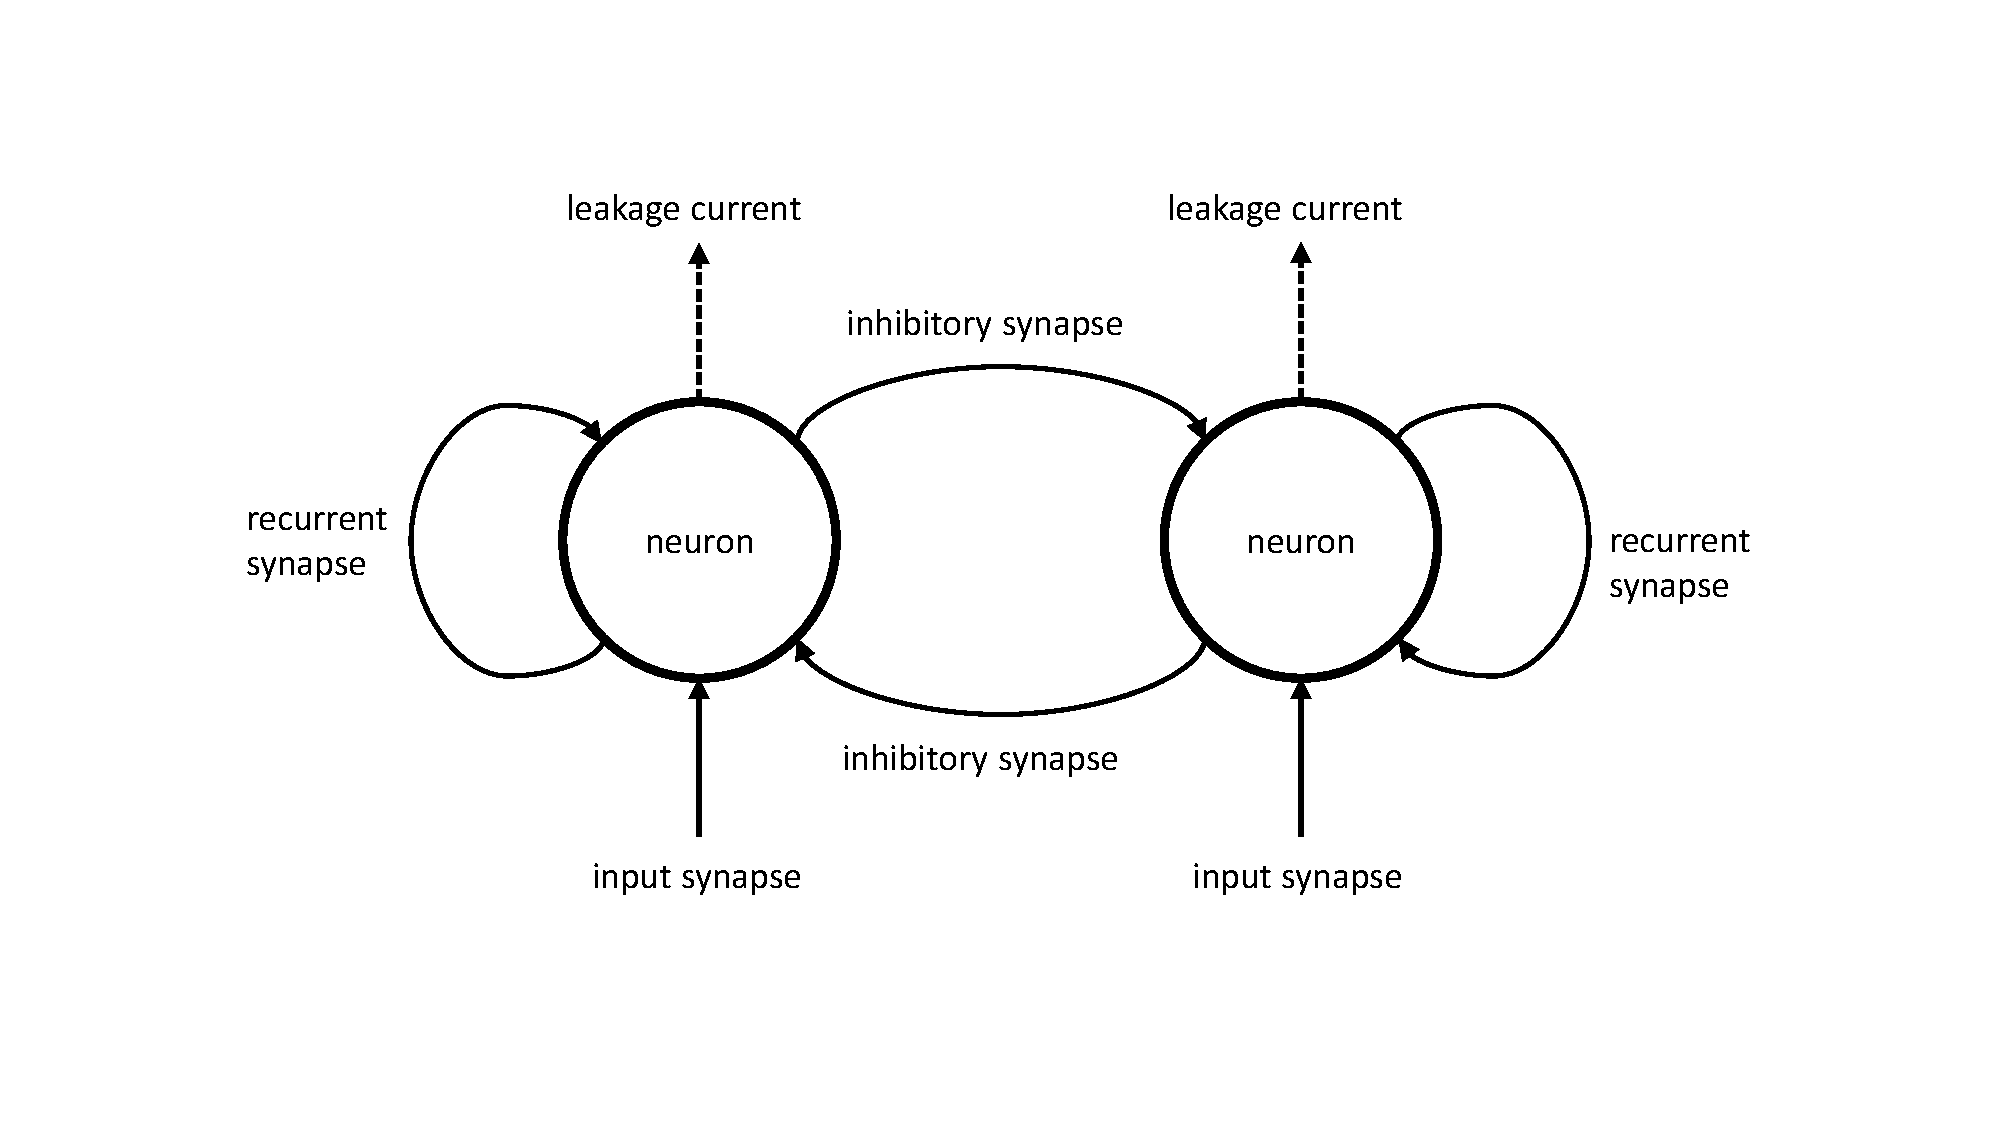
\includegraphics[width=\linewidth]{graphics/memory_cell.pdf}
        \caption{visualized Memory Cell architecture}
        \label{fig:memory_cell_vis}
    \end{figure}
    Each neuron's three synapses visible in \Cref{fig:memory_cell_vis} share the same parameters as the Memory Cell model should employ similar mechanisms when storing a $0$ or a $1$ bit.
    The behavior should be symmetric, and the decision which bit to store should only be dependent on the current input.
    The current memory content of this architecture is encoded in the potentials of both neurons.
    If the first neuron has high potential ($\approx 1$) and the second neuron low potential ($\approx 0$), the bit $1$ is currently stored, and if the second neuron has high potential ($\approx 1$) and the first neuron low potential ($\approx 0$) the bit $0$ is currently stored.
    The purpose of the input synapse, which connects the input vector entry with the synapse, is to supply each neuron with a large input current to increase its potential to $\approx 1$ if the input vector entry to the corresponding neuron is $\approx 1$, too.
    It is only applicable that at most one neuron gets a large input vector entry ($\approx 1$) at a single time step.
    This single large vector entry leads to a switch of the stored memory bit or the current memory state's persistence.
    It can also be the case that both neurons receive a small input vector entry ($\approx 0$). Therefore both neurons receive little to no input current, and the memory state is kept as ensured by the inhibitory and recurrent synapse.
    The inhibitory synapse that connects a neuron with the other neuron is responsible for suppressing the other neuron when a neuron itself has high potential. Therefore it ensures that the second neuron's potential is kept low such that only one neuron can have a high potential.
    The recurrent synapse that connects a neuron with itself is responsible that a single neuron keeps its potential if the other neuron does not inhibit it.
    Three synapses per neuron were at least necessary for a working Memory Cell architecture.
    The theoretical lower bound may be two synapses per neuron, as only an input synapse and a communication synapse that handles communication between the two neurons are needed.
    The communication synapse would be connected from one neuron to another and must fulfill the recurrent and inhibitory synapse tasks.
    However, in this scenario, with only two synapses assuming their proper functionality, the communication synapse will have to supply a negative current to inhibit the other neuron at a memory switch.
    Furthermore, when there is no memory switch, the same communication synapse must provide a positive current to a neuron with high potential to keep its state as there is a leakage current.
    The sign of a synaptic current $I_{syn,ji}$ as computed in \Cref{synaptic_current} is determined by the sign of $E_{ji} - V_i(t)$.
    The postsynaptic potential $V_i(t)$ may be $\approx 1$ in both cases, therefore the different sign of $E_{ji} - V_i(t)$ cannot be determined by the parameter $E_{ji}$ which yields a contradiction to the assumption of proper functionality.
    Each synapse from neuron $j$ to neuron $i$ has four parameters as shown in \Cref{synaptic_current}: the maximum conductance $G_{syn,ji}$, the mean conductance potential $\mu_{ji}$, the steepness of the conductance transition $\sigma_{ji}$ and the target potential $E_{ji}$.
    The steepness of the conductance transition was fixed to $100$ for all synapses in the implemented model.
    All neurons' conductances, including the leakage conductance $G_{leak}$, were parameters and therefore learned.
    The target potentials for the leakage current and the inhibitory synapse were fixed to $0$, the target potentials of the recurrent synapse and the input synapse were parameters and, therefore, also learned.
    The mean conductance potential of the input synapse was fixed to $0.5$, the mean conductance potential of the recurrent and inhibitory synapse was a parameter of the model.
    The capacitance of all neurons was fixed to $1$ and the fixed time input $t$ per time step used to integrate the state derivative in a continuous-time model was also a learned parameter.
    The state's ODE was unrolled two times per time step and was solved using the explicit Euler method.
    This unrolling is necessary such that the input currents can propagate to each of the two neurons in the first unroll step, and the inhibitory synapse currents can propagate in the second unroll step in case of a memory switch.
    Therefore, this architecture has $9$ learnable parameters.
    Validation of the model was performed using the Cell Benchmark introduced in \Cref{cell}.
    The first neuron's initial state was $0$, and the second neuron's initial state was $1$.
    The Memory Cell model implementation used in this thesis is exposed under the \texttt{get\_memory\_cell\_output} function defined in the file \url{https://github.com/Oidlichtnwoada/NeuralNetworkArena/blob/master/experiments/models/model_factory.py}.
    The in-detail implementation is provided in the file \url{https://github.com/Oidlichtnwoada/NeuralNetworkArena/blob/master/experiments/models/memory_cell.py}.


    \chapter{Benchmarks}
    In this chapter the implemented benchmark framework is first described in \Cref{benchmark_framework}.
    This framework is responsible for initiating the creation of the model, the start of the training and evalution process and the saving and visualization of the data produced during these processes.
    Then each benchmark is discussed in detail including its expected input to output data mapping, its individual command-line arguments and its specific loss function used to quantify the error a model makes.
    Four benchmarks (the Add Benchmark, the Memory Benchmark, the MNIST Benchmark and the Cell Benchmark) were used to evaluate the models' capability to capture long-term dependencies.
    These benchmarks are elaborated in \Cref{add}, \Cref{memory}, \Cref{mnist} and \Cref{cell}.
    The other two benchmarks, the Activity Benchmark and the Walker Benchmark, should test the models' capability to model dynamic physical systems.
    These two benchmarks are described in \Cref{activity} and \Cref{walker}.
    

    \section{Benchmark Framework} \label{benchmark_framework}
    The benchmark framework is split up into its four execution phases:
    \begin{itemize}
        \item{}
        Setup - prepares the model and data for training and evaluation, described in \Cref{benchmark_setup}
        \item{}
        Training - optimizes the model parameters using the given training data, described in \Cref{benchmark_training}
        \item{}
        Evaluation - evaluates the model with optimized parameters using the given evaluation data, described in \Cref{benchmark_evaluation}
        \item{}
        Data Processing - stores and visualizes data from the training and testing phase, described in \Cref{benchmark_data}
    \end{itemize}

    \subsection{Setup} \label{benchmark_setup}
    A single code base to run and evaluate the diverse set of benchmarks and models was inevitable.
    Otherwise, the whole project would have been unmanageable.
    As the implementation of all models occurred in the \texttt{Python} programming language \cite{Python3} using the framework Tensorflow \cite{Tensorflow}, also the benchmark framework used the same set of tools.
    Therefore, a benchmark base class was created in the file \texttt{benchmark.py}, which is available under the URL \url{https://github.com/Oidlichtnwoada/NeuralNetworkArena/blob/master/experiments/benchmarks/benchmark.py}.
    The creation of a new benchmark is as easy as subclassing the benchmark base class \texttt{benchmark}.
    For instructions on how to call the newly created class, please consulate the \texttt{README.md} file given under the URL \url{https://github.com/Oidlichtnwoada/NeuralNetworkArena/blob/master/README.md}.
    After subclassing the base class, the new class has to correctly call the superclass constructor and overwrite the abstract method \texttt{get\_data\_and\_output\_size}.
    Furthermore, the new benchmark's name should be added to the \texttt{BENCHMARK\_NAMES} list.
    The superclass constructor only has two arguments: \texttt{name} and \texttt{parser\_configs}.
    The first argument is just the name of the new benchmark passed as a string.
    The second argument should be a tuple of individual parser configs.
    A parser config is itself a tuple consisting of the argument name, the argument default value, and the argument type.
    This argument determines which values should be settable and usable when calling the benchmark from the command line.
    There are at least three parser configs required that set the loss name, the loss config, and the metric name.
    A sample \texttt{parser\_configs} argument would be:
    \begin{lstlisting}[language=Python]
    (('--loss_name', 'SparseCategoricalCrossentropy', str), 
     ('--loss_config', {'from_logits': True}, dict), 
     ('--metric_name', 'SparseCategoricalAccuracy', str))
    \end{lstlisting}
    If loss config or metric name does not apply to the benchmark, set the default loss config to \texttt{\{\}} or the default metric name to \texttt{''}.
    Furthermore, if the benchmark needs additional parameters, extend the \texttt{parser\_configs} parameter also to include the desired command-line arguments.
    All individual benchmark implementations use this feature.
    After calling the superclass constructor, all command-line arguments configured through \texttt{parser\_configs} will be available by their names as properties of \texttt{self.args} without the double hyphen.
    For example the loss name can be accessed by \texttt{self.args.loss\_name}.
    If some parameters were set through the command line, they would have the corresponding value. Otherwise, the configured default values will be applied.
    After that, the benchmark base class will create paths for some required directories.
    There are five directories required during benchmark execution: a saved model directory (will be created to save the models together with their best weights during training), a \texttt{TensorBoard} directory (will be created to save \texttt{TensorBoard} logs for eventual later evaluation), a supplementary data directory (already present in the repo to pass input data to the benchmark), a result directory (will be created to save CSV files with relevant information about the training process) and a visualization directory (will be created to save visualizations created after each training of a model).
    All these paths start in the root folder of the repository called \texttt{NeuralNetworkArena}.
    The structure of how these paths continue is the same for all five kinds of folders.
    For the next step in path creation, the required folder's name will be appended to the root folder.
    These names can be passed as a command argument when calling the individual benchmark classes.
    For a more detailed description of these command-line parameters, call an implemented benchmark class with the \texttt{-{}-h} command line parameter as described in the \texttt{README.md} file.
    The name of the individual benchmarks is further added to the path, such that each benchmark has its own five subfolders.
    Then the benchmark base class calls its \texttt{get\_data\_and\_output\_size} method that the subclass should have implemented.
    The function should return a tuple of inputs, a tuple of expected outputs, and an output vector size of the machine learning model.
    The input and output tuple should only contain NumPy arrays \cite{numpy}. The output tuple must have a size of precisely one.
    The input tuple must have a size of at least one.
    The benchmark base class also has support for time inputs to the models.
    Please make sure that the time input is the last entry in the input tuple.
    There is also the command line argument called \texttt{use\_time\_input}.
    If the model should use time input, make sure that this argument is set to true.
    Otherwise, if the input tuple has a dimension larger than one, the last entry will be discarded from the input tuple, as it is assumed to be the time input.
    The benchmark suite works currently only for benchmarks that provide time-series input data and only expect a model output after the last input data in the time series.
    For people familiar with the Tensorflow framework \cite{Tensorflow} this is equivalent to setting \texttt{return\_sequences=False} in an RNN model.
    All input arrays in the input tuple should have the shape \texttt{(SAMPLE\_AMOUNT, SEQUENCE\_LENGTH, INPUT\_DIMENSION)}.
    Of course, the input dimension can vary between different inputs. Time data should have an input dimension of one.
    The single output array present in the output tuple should have the shape \texttt{(SAMPLE\_AMOUNT, OUTPUT\_DIMENSION)}.
    The sample amount should match between input and output data to be valid input to the benchmark framework.
    The framework will check all the constraints on the shapes, and then all individual samples are shuffled such that corresponding input and output data are at the same indices in their arrays.
    Then tensors are created with the same shape as the input tuple's inputs, excluding the first dimension that denotes the sample amount.
    These are required to use later the Functional API of the Tensorflow framework \cite{Tensorflow}.
    They are created by specifying a fixed batch size, which helps the machine learning framework optimize the corresponding model's computational graph.
    The default batch size is set to $128$ and can be changed by a command-line parameter.
    After that, the whole samples are divided into the test, validation, and training samples. The amount of test and validation samples can be set via command line parameters, which default to $10\%$ each.
    It is ensured that each sample set is exactly divisible by the batch size, as the computational graph was optimized by only allowing inputs of a fixed batch size as described above.
    After all the setup work is done, the folder paths to the result, the saved model, and the \texttt{TensorBoard} directory will be augmented with the model name currently under test and passed via a command-line parameter.
    The \texttt{TensorBoard} directory for that model will then be deleted, as each training run creates a significant amount of log files.
    After that, the \texttt{TensorBoard}, the result, the saved model, and visualization directory will be created if they do not already exist.
    Then it will be checked if the passed model name is present in the list constant \texttt{MODEL\_ARGUMENTS} in the file \texttt{model\_factory.py}.
    When this check is passed, the benchmark framework either loads a saved model with the corresponding model name or creates a new one using the model output functions in the previously described model factory depending on the command line parameter \texttt{use\_saved\_model}.
    These output functions get an output vector size and the tensor inputs and create an output tensor that contains all the information about the operations in between.
    The Tensorflow \cite{Tensorflow} Functional API can be incorporated to create a machine learning model by knowing the input and the output tensors.
    If the model is newly created and not loaded from a saved one, the model is also compiled using a customizable optimizer, learning rate, loss, loss config, and metric.
    Command-line parameters can change these.
    The default optimizer and learning rate used throughout all benchmarks in this thesis are the Adam optimizer \cite{Adam} and a learning rate of $10^{-3}$.
    The three remaining parameters also discussed in the previous subsection must be passed such that it is conforming with the requirements of the functions \texttt{tf.keras.optimizers.get} and \texttt{tf.keras.losses.get}.
    A debug mode can also be enabled via the command line, which puts the newly created model in eager execution mode, making it easier to debug the model. Furthermore, the model will be called on a single batch of inputs without invoking the model's \texttt{fit} method. This invocation happens only in debug mode.
    In any case, a model ready to train should now have been constructed, and all the model characteristics, including input and output shape, will then be printed to the command line enabling to check if all the dimensions match the expectations.

    \subsection{Training} \label{benchmark_training}
    After printing the model's available information to the command line, a UNIX timestamp is retrieved from the system to track the total training duration.
    Then the training is ultimately started by invoking the model's \texttt{fit} method. This method takes the training and validation sample set, the batch size, the number of epochs, and a tuple of callbacks as arguments.
    The number of epochs is configurable via the command line, but the default value of $128$ is used throughout the thesis.
    The \texttt{fit} method calls the machine learning model function for each batch of inputs in the training sample set. After that, the model is validated on the validation sample set.
    Validation means the loss function is computed only on validation data, which is data that the model has never seen before.
    Validating the model should help to determine how well the model will perform on actual test data, which is also data that the model has never seen before.
    If the loss function results for training and validation data are similar, it is said that the model generalizes well.
    When the validation step is finished, the training loop proceeds with the next epoch. Therefore, it starts the same cycle again by providing the first batch of inputs from the training sample set.
    This cycle is repeated as often as the set value of the epochs.
    The callbacks are invoked after each completed epoch. There were five callbacks added:
    \begin{itemize}
        \item{}
        a \texttt{ModelCheckpoint} callback - saves the model with the best validation loss
        \item{}
        an \texttt{EarlyStopping} callback - terminates training if the validation loss has not improved for a configurable number of epochs
        \item{}
        a \texttt{TerminateOnNan} callback - terminates the training when a \texttt{nan} loss is encountered
        \item{}
        a \texttt{ReduceLROnPlateau} callback - multiplies the learning rate by a configurable factor after no improvement of the validation loss for a configurable number of epochs
        \item{}
        a \texttt{TensorBoard} callback - saves \texttt{TensorBoard} log data for eventual later inspection
    \end{itemize}
    The default number of epochs used in this thesis for the \texttt{EarlyStopping} callback is $5$.
    Another necessary callback is the \texttt{TerminateOnNan} callback, which terminates the training loop if the loss evaluates to \texttt{nan}.
    This \texttt{nan} return value can, for example, happen when the loss function diverges towards infinity, therefore, if the exploding gradient problem appears.
    It may also be the case that there is a division through zero somewhere in the computational graph, which may also lead to a \texttt{nan} loss.
    The term \texttt{nan} stands for: \texttt{not a number}.
    As all benchmarked models are trained until convergence in this thesis, the \texttt{ReduceLROnPlateau} callback is especially important.
    The corresponding default parameters are a learning rate factor of $10^{-1}$ and a default number of epochs equal to $2$, both of which are used throughout all benchmark invocations.
    The \texttt{EarlyStopping} and the \texttt{ReduceLROnPlateau} do not see an improvement if the absolute change in the validation loss is less than $0.0001$.
    This minimum delta can also be configured via the command line, but this thesis uses the default value throughout all benchmarks.
    Furthermore, all these parameters are configurable by passing alternative values in the command line.
    After the training loop has terminated, another UNIX timestamp is taken to compute the total training duration.

    \subsection{Evaluation} \label{benchmark_evaluation}
    The model is then evaluated using the parameters that led to the smallest validation loss during the whole training loop.
    Evaluation means that the model function is applied to the test sample set inputs, and the resulting loss function result on that inputs is saved.
    The created model also provides an \texttt{evaluate} method, which takes the test sample set a batch size and another callback tuple as arguments.
    The only callback passed in the tuple is the \texttt{TensorBoard} callback already used in the \texttt{fit} method invocation.

    \subsection{Data Processing} \label{benchmark_data}
    The return values of the \texttt{fit} and \texttt{evaluate} method invocations now contain information about the means of the loss and metric function results. These results are available for the training, validation, and test sample set.
    The arithmetic means for the training and validation sample set are available for each training epoch together with the currently applied learning rate.
    All information is automatically accumulated in a single CSV file per model for the training and the testing process.
    All models' testing results are also merged in a single CSV containing all model results for a single benchmark.
    Data generated during training is automatically visualized by the benchmark base class and presented in \Cref{chapter_results} that discusses the benchmark results in more detail.
    Of course, all generated files will be stored in their respective directories.


    \section{Activity Benchmark} \label{activity}
    As described in the benchmark base class, all benchmarks feature time series data where the model output is only used after the last time step to compute the loss function.
    This benchmark uses a slightly modified person activity recognition dataset from the UCI repository \cite{UCI}.
    The mentioned dataset was distributed under the \url{https://archive.ics.uci.edu/ml/machine-learning-databases/00196/ConfLongDemo_JSI.txt}.
    The target function to learn is to map a sequence of measurements from four inertial sensors worn on the person's arms and feet to an activity classification.
    This benchmark should test a model's capability to model dynamical physical systems and understand what motion patterns belong to what class.
    The ability to capture long-term dependencies is not tested with this benchmark, as the most recent input vectors should be enough to make useful predictions.
    At each time step, only the single inertial sensor's measurement is presented as input to the model.
    The model can differ between the individual sensors as the modified dataset of person activity has a one-hot encoding to mark the sensor from which the current measurement is coming.
    All benchmarks feature an additional time input, where the time interval since the last input is passed on to the model if the feature is activated.
    However, this thesis has not used an additional time input for any benchmark.
    All the measurements used for this dataset were stored in the file \texttt{activity.csv} located in the supplementary data folder described in the benchmark framework section.
    The dataset is annotated with an activity classification for each time step. However, this benchmark only requires the model to predict the classification corresponding to the last measurement data received.
    As the benchmark is a classification task, a categorical cross-entropy loss was used that was computed from the output logits of the model.
    A categorical accuracy metric is used to judge better how accurately the model predicts the activity class annotation corresponding to the last measurement input.
    Each model had an output vector size of seven, as there were seven different activity classes with their respective indices in brackets: lying ($0$), sitting on a chair ($1$), standing up ($2$), walking ($3$), falling ($4$), on all fours ($5$) and sitting on the ground ($6$).
    The processing of the UCI dataset was similarly done as in \cite{ODELSTM}.
    The benchmark had a configurable sequence length, maximum sample amount, and sample distance.
    For this thesis, a sequence length of $64$, a maximum sample amount of $40000$, and a sample distance of $4$ were used.
    The sequence length means that each model gets a history of $64$ measurements before predicting the activity corresponding to the last measurement.
    The maximum sample amount bounds the number of samples, and in the case of $40000$ samples at maximum and a sample distance of $4$, there were enough entries in the dataset file, so the benchmark was run with $40000$ samples in total.
    The sample distance is the indices offset in the dataset file between two drawn sample sequences.
    A model will get a sequence of $64$ input vectors of size seven that look like: $[0,0,0,1,4.3,1.8,0.9]$.
    The first four entries in that vector represent the one-hot encoding describing from which one of the four sensors the measurement data was taken.
    The remaining three entries contain the x, y, and z coordinate of the corresponding sensor.
    The required output vector has just one entry as it is just the index of the corresponding activity class with the mapping as described above.
    As this is a sparse class encoding, the framework has to extend this output value to a one-hot encoding to apply a cross-entropy loss between the extended one-hot encoding and our model's output vector after a softmax function was applied.
    The softmax function is necessary to convert the so-called output logits to an output probability for each class.
    The results of this benchmark are presented in a later chapter.
    The implementation of this benchmark can be found under \url{https://github.com/Oidlichtnwoada/NeuralNetworkArena/blob/master/experiments/benchmarks/activity_benchmark.py}.


    \section{Add Benchmark} \label{add}
    This benchmark uses the same structure as the Add Benchmark introduced used in \cite{UnitaryRNNs}.
    Data for this benchmark is generated randomly at each instantiation of the benchmark.
    The target function to learn is adding two marked numbers in a much longer stream of numbers.
    At each time step, a number and a marker bit are presented as an input vector to the model.
    As in the Activity Benchmark from \Cref{activity}, the sequence length and the sample amount are also configurable.
    For all models, a sequence length of $100$ and a sample amount of $40000$ was used.
    As described above, the input vector has size two.
    The second entry is set to one only in one input vector of the first and last $50$ input vectors.
    Their distribution is uniform across the whole first and second half of the time series.
    In all other input vectors, this second entry is set to zero.
    The first entry of all input vectors is filled with random numbers taken independently and uniformly from the interval $[0,1)$.
    A single input vector out of the $100$ input vectors each model gets during the benchmark looks like $[0.5,1]$.
    In this example, the random number is $0.5$, and it is marked as the second entry is one.
    As described, there are only two marked numbers, and the expected output vector has size one and is simply the addition of both marked numbers.
    This benchmark simply uses the mean squared error loss function, as the smaller the mean square error is, the more similar the expected and the model output will be.
    Furthermore, there is no metric used in this benchmark.
    As this benchmark uses an increased sequence length of $100$ and the error signal is only provided after the last input vector, the model will only learn this function when capturing long-term dependencies.
    This condition means the model function must be designed so that the gradient does not vanish or explode during backpropagation through the model's function.
    These problems were discussed in detail in \Cref{long_term_difficult}.
    When the model cannot capture these long-term dependencies and cannot store seen marked values in its state, it will be forced to learn the naive memory-less strategy of always predicting one.
    Predicting $1$ will be the case in this strategy as the expectation of each unique number out of the two marked ones is $0.5$, as they were drawn uniformly from the given interval.
    The addition of both expectation values reveals the output of the memory-less strategy.
    As also pointed out in \cite[p. 6]{UnitaryRNNs}, this naive strategy will lead to a mean squared error of $\frac{1}{6}$.
    This result can be verified as the mean squared error when predicting the mean equals the distribution's variance.
    As both random numbers were picked independently of each other, the random number sum's variance is just the sum of their variances.
    The distribution from which the random numbers are drawn has variance $\frac{1}{12}$.
    Therefore, adding this value to itself proves the mean square error of the memory-less strategy.
    For this benchmark, the model output vector size is simply one, as it should just contain the sum of both marked numbers.
    The results of this benchmark are presented in a later chapter.
    The implementation of this benchmark can be found under \url{https://github.com/Oidlichtnwoada/NeuralNetworkArena/blob/master/experiments/benchmarks/add_benchmark.py}.


    \section{Walker Benchmark} \label{walker}
    This benchmark evaluates how well a model can predict a dynamic, physical system's behavior. It was taken from \cite{ODELSTM}.
    The training data is acquired simulation data of the \texttt{Walker2d-v2} OpenAI gym \cite{OpenAIGym} controlled by a pre-trained policy.
    The objective was to learn the MuJoCo physics engine's kinematic simulation \cite{MuJoCo} in an auto-regressive fashion using imitation learning.
    The simulation data was acquired from various training stages of the pre-trained policy (between 500 and 1200 Proximal Policy Optimization iterations) to increase the task difficulty. Furthermore, 1\% of actions were overwritten by random actions.
    The simulation environment can be visualized as follows:
    \begin{figure}[H]
        \centering{}
        \includegraphics[page=7,width=0.8\linewidth,trim={340 345 105 375},clip]{literature/learning_long_term_dependencies_in_irregularly_sampled_time_series.pdf}
        \caption{visualized \texttt{Walker2d-v2} OpenAI gym \cite[p. 7]{ODELSTM}}
        \label{fig:walker2d_vis}
    \end{figure}
    Furthermore, the benchmark implements eventual frame-skips that would create an irregularly sampled time series.
    This feature was not used in this thesis as it covers only regularly sampled time series.
    If the model understands the dynamics guided by differential equations, it will produce accurate predictions.
    The ability to capture long-term dependencies is not tested with this benchmark, as the most recent input vectors should be enough to make good predictions.
    The benchmark had a configurable sequence length, a maximum sample amount, and a sample distance, just like the Activity Benchmark from \Cref{activity}.
    Throughout the thesis, a sample length of $64$, a maximum sample amount of $40000$, and a sample distance of $4$ were used.
    All parameters have the same meaning as before.
    There was enough training data provided in \texttt{.npy} files by the creators of \cite{ODELSTM}, therefore $40000$ different samples were available that were partitioned in training, validation, and test samples.
    The acquired simulation data can be downloaded from \url{https://pub.ist.ac.at/~mlechner/datasets/walker.zip}.
    The input sequence consists of input vectors of size $17$, which contains the physics engine's current state at this specific time step.
    These values represent the angles of the joints and the absolute position of the bipedal robot.
    The function to learn for this benchmark is to predict the physics engine's state in the next time step by giving the machine learning model history of the past $64$ physic engine's states.
    Therefore, the model output vector size was set to $17$, and the expected output data were also vectors of size $17$.
    As both vectors have the same size and the more similar they are, the better the prediction is, a mean squared error loss was used.
    There was no metric used for this benchmark.
    The results of this benchmark are presented in a later chapter.
    The implementation of this benchmark can be found under \url{https://github.com/Oidlichtnwoada/NeuralNetworkArena/blob/master/experiments/benchmarks/walker_benchmark.py}.


    \section{Memory Benchmark} \label{memory}
    This benchmark evaluates how well a model can capture long-term dependencies by letting the model recall past seen categories exactly.
    It is a slightly changed version of the copying memory problem described in \cite{UnitaryRNNs}.
    Input data of the benchmark input is randomly created at each invocation of the benchmark.
    There is a configurable memory length to test for, a configurable length of the sequence to memorize, a configurable number of categories, and a configurable number of randomly generated samples.
    The benchmark had set the memory length to $100$, the sequence length to $1$, the category amount to $10$, and the sample amount to $40000$ throughout the thesis.
    Each single input vector sequence is created by concatenating three subsequences.
    The first sequence is the sequence to memorize of length $1$.
    It contains category indices sampled uniformly from $0$ to $9$.
    The second sequence is then just a sequence of the filler symbol $10$ repeated $100$ times.
    The third sequence is just the index of the category in the sequence to memorize what the model should recall, which is also sampled uniformly from all available indices in the sequence.
    This sequence is obviously of length $1$ and always filled with $0$ in the previously described setup.
    In total, this makes up for a total sequence length of $102$ and a vector size of $1$ per time step.
    The expected output category is encoded sparsely as in the Activity Benchmark from \Cref{activity} and contains a category index from $0$ to $9$ that matches the category at the index the model got the last time step in the sequence to memorize.
    The model's output vector size is $10$, and each output logit represents a single category.
    As this is a classification problem, a categorical cross-entropy loss was used between the model's output logits passed through a softmax function and the one-hot encoding extension of the sparsely encoded expected category index.
    To better visualize how good a model can recall the category, a categorical accuracy metric was added to this benchmark.
    It must be pointed out that a model is only capable of recalling the category seen in the first input vector if the gradient does not vanish or explode, as the error signal is only provided after the last time step.
    A model that cannot capture the long-term dependencies in this benchmark will be forced to learn the memory-less strategy, which entails that all output logits have the same value, i.e., all categories are equally likely.
    This will lead to a categorical crossentropy loss of $-\ln{\frac{1}{10}} \approx 2.303$ and a sparse categorical accuracy of roughly $0.1$.
    The results of this benchmark are presented in a later chapter.
    The implementation of this benchmark can be found under \url{https://github.com/Oidlichtnwoada/NeuralNetworkArena/blob/master/experiments/benchmarks/memory_benchmark.py}.


    \section{MNIST Benchmark} \label{mnist}
    This benchmark evaluates how well a model can capture long-term dependencies. For correct classification, the model needs to incorporate input vectors from the distant past, further explained below.
    The idea to incorporate this benchmark was taken from \cite{ODELSTM}, which also features an event-based sequential MNIST classification problem.
    Input sequences for this benchmark were constructed from the MNIST dataset \cite{mnist} of the Keras framework \cite{Keras}.
    The MNIST dataset contains images of hand-drawn digits of $28$ by $28$ pixels where a single integer encodes each pixel from $0$ to $255$.
    All images are in grey-scale, and a higher integer represents a darker pixel.
    Some examples of these images are given in the following figure:
    \begin{figure}[H]
        \centering{}
        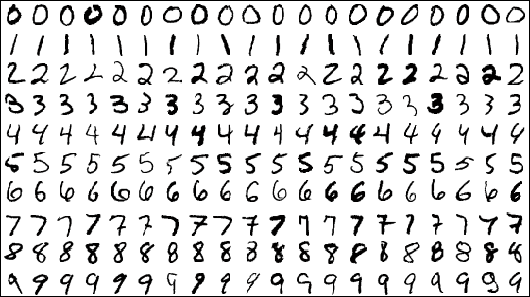
\includegraphics[width=0.8\linewidth]{graphics/mnist.png}
        \caption{images from the MNIST dataset \cite{mnist}}
        \label{fig:mnist_vis}
    \end{figure}
    The images were vectorized to a vector containing $784$ entries and then split up to a sequence of vector chunks of size $8$, which results in an input sequence length of $98$.
    The expected output class index is just the digit the current image is representing.
    Furthermore, the benchmark has a configurable maximum amount of samples, which was set to $40000$.
    As the MNIST dataset had enough image samples, all specified $40000$ samples were used.
    Long-term memory of seen input chunks is necessary to produce an accurate category prediction, as digits like $1$, $4$, and $9$ may be indistinguishable when only considering the most recent seen input chunks.
    This limitation corresponds to classifying the image only based on a lower fraction of the image visible to the model, where the upper fraction was cut away.
    A model that yields accurate results must not suffer from the vanishing or exploding gradient problem, as only then the whole picture can be taken into account for classification.
    The model output vector size was set to $10$, as each output logit should represent a single digit.
    As the expected output digit is encoded sparsely, the same procedure as in the Memory Benchmark from \Cref{memory} is applied to compute the categorical cross-entropy loss.
    The models' performance was also measured using a categorical accuracy metric, which produces a more human-interpretable result than the chosen loss function.
    The results of this benchmark are presented in a later chapter.
    The implementation of this benchmark can be found under \url{https://github.com/Oidlichtnwoada/NeuralNetworkArena/blob/master/experiments/benchmarks/mnist_benchmark.py}.


    \section{Cell Benchmark} \label{cell}
    This benchmark evaluates if the newly introduced Memory Cell architecture can repeatedly store a single bit of information, including switching the memory state.
    Furthermore, it should be checked if the memory state vanishes or successfully persists over a long time horizon.
    Memory persistence requires capturing long-term dependencies as the input is provided sparsely to the model as described below.
    The benchmark has a configurable memory high symbol, memory low symbol, memory length, amount of cell switches, and samples generated at each benchmark invocation.
    The memory high and low symbols represent the expected output symbol when either memory state is active, but the memory high symbol is also used as an input symbol to activate a specific memory state sparsely. All other inputs are then set to the memory low symbol.
    The memory high symbol was picked to $1$, the memory low symbol was picked to $0$, the memory length was picked to $128$, the number of cell switches was set to $2$, and the sample amount was set to $40000$.
    As the Memory Cell architecture is a bistable memory element, two memory states can be activated sparsely.
    The input vector at each time step has a size of $2$. If both entries are $0$, the current memory state should be kept.
    Otherwise, if a single entry is $1$ and the other entry is $0$, the corresponding memory state should be activated.
    The first part of the input sequence is constructed by activating any of the memory states sparsely, and the succeeding $127$ vectors are all-zero vectors.
    This subsequence now has a length of $128$. The following sequence is built like the first one, but it activates the cell not activated initially, which corresponds to a cell switch.
    There are $2$ further subsequences of this kind. The final input sequence is then the concatenation of all three subsequences and has a length of $384$.
    In half of the samples, either memory state is activated first in the concatenated sequence.
    The required model output vector is also given as a sequence of vectors of size $2$. Therefore the error signal is provided at each time step.
    The output sequence can be quickly built from the input sequence by continuing to set its entry to $1$ at the corresponding index until a new sparsely input is provided to the model.
    Therefore, the model may get the input sequence consisting of the following vectors: $[1,0],[0,0],[0,0],...,[0,1],[0,0],[0,0]$ and is required to produce the following vectors of the expected output sequence: $[1,0],[1,0],[1,0],...,[0,1],[0,1],[0,1]$.
    The sparse activation of the Memory Cell should lead to permanent storage of the activation until a new sparse input is provided to the model.
    As described above, the model output vector size is $2$, and a mean squared error loss without a metric was used, as more similar vectors lead to a better prediction.
    The results of this benchmark are presented in a later chapter.
    The implementation of this benchmark can be found under \url{https://github.com/Oidlichtnwoada/NeuralNetworkArena/blob/master/experiments/benchmarks/cell_benchmark.py}.


    \chapter{Results} \label{chapter_results}
    In this chapter the used benchmark hardware is first specified in \Cref{benchmark_hardware} which also includes the overall structure of the experiments.
    After that the results of all models for each benchmark are discussed in detail.
    This discussion per benchmark includes an elaboration on the relative performances of all models, a result summary presented in a table and a plot showing the validation loss evolution of all models for this benchmark and a single run.
    The results of the Activity Benchmark are presented in \Cref{activity_results}, the results of the Add Benchmark are presented in \Cref{add_results}, the results of the Walker Benchmark are presented in \Cref{walker_results}, the results of the Memory Benchmark are presented in \Cref{memory_results}, the results of the MNIST Benchmark are presented in \Cref{mnist_results} and the results of the Cell Benchmark are presented in \Cref{cell_results}.


    \section{Benchmark Hardware and Experiment Clarifications} \label{benchmark_hardware}
    The benchmark server was equipped with an \texttt{AMD Ryzen Threadripper 2970WX} $24$-core processor and two \texttt{NVIDIA Titan RTX} graphics cards.
    Software-wise, the system used the \texttt{Ubuntu 18.04.5 LTS} operating system and a \texttt{Python 3.8.7} \cite{Python3} interpreter to execute all Python scritps.
    The used \texttt{Tensorflow} \cite{Tensorflow} library had version \texttt{2.4.1}, the used \texttt{NVIDIA CUDA} library had version \texttt{11.0.3}, the used \texttt{NVIDIA cuDNN} library \cite{cuDNN} had version \texttt{8.0.5.39}, the used \texttt{NVIDIA TensorRT} library had version \texttt{7.2.2} and the \texttt{NVIDIA} GPU driver had version \texttt{460.32.03}.
    All benchmarks were started using the script \texttt{run\_all\_benchmarks\_and\_models.py} which invokes all applicable benchmark and model combinations once.
    The CPU and both GPUs were used as computing devices during training.
    The script can be found under the URL \url{https://github.com/Oidlichtnwoada/NeuralNetworkArena/blob/master/run_all_benchmarks_and_models.py}.
    This script was executed three times, and the produced log data was processed using the script \texttt{apply\_and\_save\_statistics.py} which extracted the statistics (means and standard deviations) in CSV files out of all measured metrics.
    Time metrics are always reported in seconds.
    All values in the measured metrics are reported with a precision of three decimal digits.
    The test loss of models is reported in brackets after their names in the following sections.
    This script can be found under the URL \url{https://github.com/Oidlichtnwoada/NeuralNetworkArena/blob/master/apply_and_save_statistics.py}.
    To achieve transparency on how the results were obtained, all logs generated during the three runs are available under \url{https://github.com/Oidlichtnwoada/NeuralNetworkArena/tree/master/benchmark_logs}.


    \section{Activity Benchmark} \label{activity_results}
    The statistics summary for this benchmark is shown in \Cref{tab:test_loss_activity} and the validation losses during training for all models are visualized in \Cref{fig:validation_loss_activity}.
    This benchmark should test whether a model can model a dynamic physical system.
    The Activity Benchmark is considered to be solved when the categorical accuracy is higher than $0.9$.
    The Transformer architecture achieved the lowest test loss of $0.178$ and highest accuracy of $0.937$ by incorporating the great expressivity of multi-head attention and the concept of attention.
    Therefore, the Transformer architecture learns that more recent measurement data will have a more considerable impact on the final classification than measurement data from the distant past.
    The Transformer architecture is followed by the GRU ($0.209$), CT-GRU ($0.223$), DNC ($0.229$), ODE-LSTM ($0.235$) and LSTM ($0.245$) architecture which all delivered a good test loss.
    This benchmark reveals that GRU and LSTM architectures are not only good in memory-related tasks but can also be used to model a sampled physical system.
    Remarkably, the GRU architecture, which simplifies the LSTM architecture, outperformed its mother architecture by trading model complexity for hidden state size.
    Furthermore, the continuous-time variant of the LSTM, the ODE-LSTM, was better suited to model the physical system than the vanilla LSTM architecture, but it also had a larger parameter count.
    The DNC architecture performed comparatively to the CT-GRU architecture, and the LSTM architecture is followed by the Memory Augmented Transformer ($0.257$).
    The DNC and the Memory Augmented Transformer employ an external memory and separate computation from memory.
    Therefore, they solve each benchmark task by meta-learning, which is a synonym for learning to learn.
    Gradient descent learns an algorithm to solve each task in these models instead of learning the function that maps input data to output data directly.
    The DNC has a far more complex model function than the Memory Augmented Transformer and is far more constrained in its operations.
    These restrictions result in a better test loss than the Memory Augmented Transformer, but the latter also performed exceptionally well with less trainable parameters.
    Worth mentioning is that all mentioned models except the DNC and Memory Augmented Transformer trained very quickly. The two exceptions needed at least a full hour to train the required function.
    Until now, all architectures were able to solve the benchmark, i.e., reached a categorical accuracy of more than $0.9$, all succeeding models failed to do so.
    The next best architecture was the Matrix Exponential Unitary RNN ($0.336$) in its full-space configuration, which outperformed the regular Unitary RNN in test loss and training duration, though both training durations were quite long.
    As the regular Unitary RNN in its full-space configuration took too long to train, it was benchmarked in its partial-space configuration, therefore the parameter count difference.
    It should be visible that the unitary matrix parameterization with a matrix exponential is computationally more efficient than the approach with rotational matrices.
    The Matrix Exponential Unitary RNN architecture is followed by the Recurrent Network Augmented Transformer ($0.373$) and the Recurrent Network Attention Transformer ($0.410$).
    The hypothesis of adding more expressivity to the Transformer architecture by accumulating the weighted value vectors with an LSTM in the Recurrent Network Augmented Transformer is not valid in this case.
    The same statement holds for the newly introduced recurrent network attention using Unitary RNNs used in the Recurrent Network Attention Transformer.
    As both modifications dramatically increase model complexity and training duration compared to the standard Transformer architecture, they are not a viable option for this kind of real-world application.
    The next best model was the CT-RNN ($0.510$), followed by the Unitary RNN architecture ($0.522$).
    Both architectures have not performed well on this benchmark and needed a long time to train.
    The CT-RNN architecture should be capable of modeling physical systems as discussed in \Cref{physical_systems}.
    The hypothesis is that the additional classification task on top of the physical system modeling was the high test loss's culprit.
    Perhaps the Matrix Exponential Unitary RNN benefits from using the imaginary part of its hidden state when projecting it to the model output vector using a dense layer.
    The two remaining models, the Unitary NCP ($0.573$) and NCP ($1.088$) architecture, performed very poorly on this benchmark and took a significant amount of time to train.
    Due to the NCP architecture's complex model function, both models had a small number of neurons that were very sparsely connected with chemical synapses to train them in a reasonable time.
    This sparseness is a likely reason for the high test loss of both models.
    Future papers should work on approximations or simplifications of the LTC network architecture, such that more extensive networks are trainable in a reasonable time.
    \benchmarksummary{activity}{Activity}


    \section{Add Benchmark} \label{add_results}
    The statistics summary for this benchmark is shown in \Cref{tab:test_loss_add} and the validation losses during training for all models are visualized in \Cref{fig:validation_loss_add}.
    This benchmark should test whether a model can capture long-term dependencies in time series.
    The adding problem is considered to be solved when the mean test loss is under $0.04$.
    The same models as reported in \Cref{activity_results} take a significant amount of time to train. Therefore, only exceptions to the norm in terms of training duration will be reported in the following.
    The Transformer architecture achieved the perfect test loss of $0.000$ by incorporating the concept of attention as discussed in \Cref{activity_results}.
    This architecture processes all input vectors of the input vector sequence at once and does not need to save each input vector at a single time step in its hidden state in encoded form.
    Therefore, it can simply focus on the two marked input vectors in the sequence and add them together without repeatedly applying a model function at each time step.
    The Recurrent Network Augmented Transformer also achieved the perfect test loss of $0.000$ by applying the attention mechanism to the input sequence.
    The added model complexity of the additional RNN in this architecture has not prevented it from learning the correct model function.
    The next best model was the GRU architecture ($0.001$), followed by the CT-GRU architecture ($0.001$). Both of which performed very well on this benchmark.
    They both outperformed their LSTM counterparts, given by the LSTM and ODE-LSTM architecture.
    Furthermore, the Recurrent Network Attention Transformer ($0.002$) also performed very well on this task.
    It uses the introduced recurrent network attention mechanism and a Unitary RNN, and this combination has beaten the vanilla Unitary RNN architecture in terms of test loss.
    This architecture is followed by the DNC ($0.007$), the CT-RNN ($0.019$), and the Matrix Exponential Unitary RNN architecture ($0.022$).
    The DNC learned the desired function using meta-learning and saved the marked values to its external memory. Surprisingly, the CT-RNN architecture was also able to learn the add function, even though the architecture has no gating mechanism like the LSTM or GRU architecture and no bounded loss gradient like the Unitary RNNs.
    The Matrix Exponential Unitary RNN was also able to learn the add function and training was significantly more stable than for the standard Unitary RNN as measured by the test loss standard deviation of $0.032$ compared to $0.076$.
    As in the Activity Benchmark, the Matrix Exponential Unitary RNN has outperformed the Unitary RNN in test loss and training duration.
    The following models are the LSTM ($0.066$), the Unitary RNN ($0.094$), the Unitary NCP ($0.106$), and the Memory Augmented Transformer architecture ($0.122$).
    These models are not considered to have solved the adding problem as their test loss is larger than $0.04$.
    All four test loss standard deviations of these models are relatively high (larger than $0.075$) because they have solved the adding problem in some benchmark runs, whereas, in the other benchmark runs, they failed to do so.
    In the LSTM and Unitary RNN architecture case, ill-suited initialization values may cause different behaviors on different runs, hindering the optimizer from finding suitable parameters for the models.
    The Matrix Exponential Unitary RNN always initializes its matrix $W$ to the identity matrix, which somehow helps the optimizer tune the model's parameters in this benchmark task.
    Ill-suited initialization values are also a possible cause in the Unitary NCP and Memory Augmented Transformer architecture, but for the Unitary NCP architecture, the very sparsely connected neurons discussed in \Cref{activity_results} may also be a problem.
    The Memory Augmented Transformer architecture may smoothen its loss surface, which helps the optimizer by setting its embedding size equal to the vector size stored in each memory row.
    Then the memory embedding can be omitted, and its parameters can be used for the multi-head self-attention mechanism.
    Furthermore, the memory control dense layer may use a residual connection to specify the memory change instead of building a new memory row vector from scratch at each time step when the enable signal is active.
    The worst two models which were only able to learn the memory-less strategy discussed in \Cref{add} are the NCP ($0.166$) and the ODE-LSTM model ($0.167$).
    As the NCP architecture has no bounded loss gradient, it suffers from the vanishing gradient problem as discussed in \cite[p. 2]{NCP} and therefore cannot memorize the two marked numbers.
    The sparsity problem also applies here.
    The Unitary NCP architecture performed better on this task because it incorporates a Unitary RNN for memory-related tasks.
    Surprisingly, the ODE-LSTM architecture was not able to capture the long-term dependencies in this benchmark task.
    Somehow the added CT-RNN in its architecture changed the loss surface such that it is more difficult for the optimizer to find suitable parameters.
    \benchmarksummary{add}{Add}


    \section{Walker Benchmark} \label{walker_results}
    The statistics summary for this benchmark is shown in \Cref{tab:test_loss_walker} and the validation losses during training for all models are visualized in \Cref{fig:validation_loss_walker}.
    This benchmark should test whether a model can model a dynamic physical system.
    The Walker Benchmark is considered to be solved when the test loss is smaller than $1.5$.
    The ODE-LSTM architecture achieved the lowest test loss of $1.159$ by incorporating the capability to model physical systems of the CT-RNN and the capability to capture long-term dependencies of the LSTM architecture.
    Even though the most recent states accurately determine the next state of the physics simulation, additional memory helps in this task as the CT-RNN is the only second best architecture with a test loss of $1.205$, but with a smaller parameter count.
    This architecture seems to benefit from its model structure as hypothesized in \Cref{physical_systems}, as the benchmark task is just about finding the input-output relation of a physical system without an additional classification task.
    The next best architectures were the Memory Augmented Transformer ($1.213$) and the DNC ($1.330$).
    Both of these architectures have an external memory and employ meta-learning.
    Surprisingly, the Memory Augmented Transformer, with its more flexible model function when compared to the DNC, achieved a lower test loss in this benchmark.
    The DNC was followed by the GRU ($1.339$), the LSTM ($1.363$), and the CT-GRU ($1.526$) architecture, which all performed exceptionally well on this benchmark task.
    Until the LSTM all architectures could solve the benchmark, i.e., reached a test loss of less than $1.5$, all succeeding models failed to do so.
    It seems that employing continuous-time models like the ODE-LSTM helps to achieve better results than employing discrete-time models even when regularly sampled input data is used.
    This ability to generalize to arbitrary time inputs of continuous-time models is discussed in \Cref{odelstm} and computing the state change may be easier than computing a new state at each time step.
    The next best architecture was the Transformer which achieved a test loss of $1.599$.
    This benchmark task seemed challenging for the Transformer architecture, as maybe the positional encoding cannot be appropriately incorporated when attention to several individual positions is required.
    That is probably why recurrent neural network architectures perform better on this task, as they naturally incorporate positional information in their model functions.
    This deficiency of the Transformer was not such a significant issue in the Activity Benchmark from \Cref{activity_results}, as the activity labels changed very infrequently.
    The Transformer was followed by the Unitary RNN ($1.622$), which outperformed the Matrix Exponential Unitary RNN in this benchmark.
    Probably, a partial-space unitary matrix $W$ and the different parametrization helps with this benchmark.
    The following two models in the ranking were the Recurrent Network Augmented Transformer ($2.207$) and the Recurrent Network Attention Transformer ($2.490$).
    Both architectures should augment the Transformer architecture in different ways by adding RNNs to it, which should help with exact positional information.
    As the test loss of both architectures is relatively high, this idea has not worked.
    The Matrix Exponential Unitary RNN was the next model with a test loss of $3.180$ and an outstanding high test loss standard deviation of $1.406$.
    In one benchmark run, the model even achieved a comparative test loss to the Unitary RNN.
    Maybe an improved initialization strategy helps to stabilize training for this model.
    The worst two models were the Unitary NCP ($3.438$) and the NCP ($4.850$) architecture, which both suffered from their sparsely connected few neurons.
    \benchmarksummary{walker}{Walker}


    \section{Memory Benchmark} \label{memory_results}
    The statistics summary for this benchmark is shown in \Cref{tab:test_loss_memory} and the validation losses during training for all models are visualized in \Cref{fig:validation_loss_memory}.
    This benchmark should test whether a model can capture long-term dependencies in time series.
    The Memory Benchmark is considered to be solved when the categorical accuracy is higher than $0.9$.
    Four architectures achieved the perfect categorical accuracy of $1.000$: the Unitary RNN ($0.000$), the Recurrent Network Attention Transformer ($0.008$), the Matrix Exponential Unitary RNN ($0.062$) and the Unitary NCP architecture ($0.205$).
    The Unitary RNN has outperformed the Matrix Exponential Unitary RNN, which has again a problem with a high test loss standard deviation of $0.042$ when compared to $0.000$ of the Unitary RNN.
    This problem was also discussed in \Cref{walker_results}, and a partial-space unitary matrix $W$ might be easier to handle by the optimizer.
    The Unitary RNN trained very quickly, and with its bounded loss gradient, it also helped the Recurrent Network Attention Transformer and the Unitary NCP architecture produce excellent results.
    The last architecture that solved the benchmark was the Recurrent Network Augmented Transformer ($0.205$) with a categorical accuracy of $0.966$.
    It is impressive that both Transformer derivative models outperformed their mother architecture by better incorporating positional information and an RNN with bounded loss gradient.
    The Recurrent Network Augmented Transformer even outperformed the LSTM architecture, though its core uses an LSTM to accumulate the attention mechanism's weighted value vectors.
    The Unitary NCP does an excellent job of delegating this memory-related task to the Unitary RNN.
    The next best model was the CT-GRU ($0.321$), followed by the Transformer ($0.362$), the GRU ($0.768$), and the DNC architecture ($1.534$).
    These models were able to solve the Memory Benchmark in some benchmark runs and failed in other runs, leading to a high test loss standard deviation of all these models.
    Maybe an improved initialization strategy for these models helps with this problem.
    Surprisingly, the Transformer architecture could not solve the Memory Benchmark in every run, though it needs to attend to the first input vector containing the required category.
    This lousy result means that the Transformer's positional encoding might not work as reliable as expected in \cite[p. 5-6]{Transformer}.
    The worst models which only learned the memory-less strategy discussed in \Cref{memory} were the Memory Augmented Transformer, the LSTM, the NCP, the CT-RNN, and the ODE-LSTM architecture, all of which have achieved a test loss of $2.303$ and a categorical accuracy of roughly $0.1$.
    The Memory Augmented Transformer may improve its performance by incorporating the changes discussed in \Cref{add_results}.
    Outstandingly, both LSTM architectures failed to solve the benchmark, even though they employ gating on their cell state.
    Not very surprisingly, the NCP and CT-RNN architecture failed to solve the task, as none has bounded loss gradient, and therefore both suffer from the vanishing gradient problem.
    If the gradients were exploding, the training loop would have terminated itself as specified by the \texttt{TerminateOnNan} callback described in \Cref{benchmark_framework}.
    \benchmarksummary{memory}{Memory}


    \section{MNIST Benchmark} \label{mnist_results}
    The statistics summary for this benchmark is shown in \Cref{tab:test_loss_mnist} and the validation losses during training for all models are visualized in \Cref{fig:validation_loss_mnist}.
    This benchmark should test whether a model can capture long-term dependencies in time series.
    The MNIST classification problem is considered to be solved when the categorical accuracy is higher than $0.9$.
    The DNC architecture achieved the lowest test loss of $0.201$ by incorporating meta-learning and its external memory, and it also achieved the highest categorical accuracy of $0.940$.
    As mentioned in \Cref{activity_results}, this architecture learns an algorithm to solve the problem by gradient descent, and this approach seems to work quite well on this task.
    The other models able to solve the benchmark were the GRU ($0.221$), the LSTM ($0.285$), and the Unitary RNN architecture ($0.365$).
    The Recurrent Network Attention Transformer had a slightly lower test loss than the Unitary RNN with $0.345$, but its categorical accuracy was slightly lower than $0.9$ with $0.893$.
    As the Unitary RNN has bounded loss gradient and performs exceptionally well on this benchmark, the Transformer derivative model that uses it performed well, too.
    The GRU and LSTM architecture's gating mechanism seems to work as expected in this benchmark, and as in the memory-related Add Benchmark, the ODE-LSTM performed worse than the vanilla LSTM architecture.
    It seems that the additional postprocessing of the hidden state vector with a CT-RNN in the ODE-LSTM has a negative influence on the gating mechanism in memory-related tasks.
    The next best model was the ODE-LSTM ($0.372$) followed by the CT-GRU ($0.588$), the Transformer ($0.654$), the Matrix Exponential Unitary RNN ($0.712$), and the Recurrent Network Augmented Transformer architecture ($0.754$).
    These models could not solve the benchmark task as defined, but they all delivered decent results.
    Interestingly, the CT-GRU with its multi-dimensional exponentially decaying state performs worse than the vanilla GRU model, even though it was constructed to generalize the GRU architecture.
    The Transformer architecture should have also performed better on this benchmark, as it could merely attend to image chunks that are different between the ten digits.
    As this was not the case, the hypothesis that the positional encoding might not work as expected formulated in \Cref{memory_results} is further strengthened.
    The Recurrent Network Augmented Transformer, designed to be a generalization of the Transformer architecture, performed worse than its mother architecture and did not show any advantages in this benchmark task.
    The Unitary RNN outperformed the Matrix Exponential Unitary RNN in this benchmark, which only uses a partial-space unitary matrix $W$, and this seems to ease optimization.
    The worst models in this benchmark were the CT-RNN ($1.164$), the Memory Augmented Transformer ($1.313$), the NCP ($1.624$), and the Unitary NCP architecture ($1.876$).
    As already discussed in \Cref{memory_results}, the CT-RNN and NCP architecture both suffer from the vanishing gradient problem, which leads to wrong classifications.
    Furthermore, the sparsely connected few neurons in the NCP and Unitary NCP architecture may be a reason for inferior performance compared to other models.
    The Memory Augmented Transformer could not apply the concept of meta-learning as effectively as the DNC in this benchmark, but it may improve its performance by incorporating the changes discussed in \Cref{add_results}.
    \benchmarksummary{mnist}{MNIST}


    \section{Cell Benchmark} \label{cell_results}
    The statistics summary for this benchmark is shown in \Cref{tab:test_loss_cell} and the validation loss during training for the Memory Cell is visualized in \Cref{fig:validation_loss_cell}.
    This benchmark should test whether the Memory Cell architecture can capture long-term dependencies in time series.
    This ability was present as the Memory Cell achieved a perfect test loss of $0.000$ in each of the three benchmark runs with a test loss standard deviation of $0.000$.
    The total amount of epochs to train was relatively low with $6$ as the Memory Cell's initialization values were picked close to a local minimum. Otherwise, the loss gradient kept diverging.
    This test loss result validates that the architecture described in \Cref{memory_cell} is indeed able to capture long-term dependencies in time series similar to the input time series of the Cell Benchmark introduced in \Cref{cell}.
    A downside of the architecture is the training duration of nearly two minutes per epoch for an architecture that only has $9$ trainable parameters.
    The Cell Benchmark featured an input sequence length of $384$ and $40000$ samples in total.
    Therefore, there is lots of future work to do to speed up this model's training using simplifications or approximations in the model function.
    Another open question is how to intelligently couple multiple Memory Cells together. A further question is if these Memory Cells should be coupled tightly or instead loosely like the memory bits in our personal computers.
    Furthermore, a controller should be introduced like the one in the DNC architecture that provides suitable input currents to the Memory Cells.
    \benchmarksummary{cell}{Cell}


    \chapter{Summary and Future Work}
    The Transformer architecture has a superior expressivity but shows deficiencies in tasks where exact positional information is required.
    Possible future research should be directed on how the Transformer architecture can more effectively use the positional data in input time series.
    The GRU and LSTM architecture showed that the gating mechanism works as expected in most cases, and the GRU architecture is a meaningful simplification of the LSTM architecture.
    The GRU architecture outperformed the LSTM architecture by trading in model complexity for hidden state size in all benchmarks.
    In most benchmarks, the CT-GRU performed comparatively to the vanilla GRU and did not show increased performance due to the more general model function.
    The ODE-LSTM was especially good on tasks invoking dynamic physical systems but showed deficiencies in memory-related tasks.
    The Unitary RNN and Matrix Exponential Unitary RNN performed very well on memory-related tasks but had their problems modeling physical systems.
    Some problems might be mitigated by researching how to initialize these models better.
    Furthermore, the influence of both models' used capacities on the test loss would be quite interesting.
    The benchmarks showed that the unitary matrix parameterization with a matrix exponential is computationally more efficient than the approach with rotational matrices used in \cite{EfficientUnitaryRNNs}.
    The DNC architecture employed the meta-learning mechanism more effectively than the Memory Augmented Transformer, most likely because of its more constrained memory operations.
    The Memory Augmented Transformer also showed some promising results, but training is not stable enough.
    It would be interesting to implement the possible improvements mentioned in \Cref{add_results} in future work and evaluate their effect on test loss and training stability.
    The Recurrent Network Augmented Transformer and the Recurrent Network Attention Transformer, both Transformer derivatives, performed inferior in all tasks where the Transformer architecture delivered good results.
    In tasks where the Transformer architecture struggled, the added RNNs in these architectures helped both to achieve superior results compared to the Transformer in some cases.
    Furthermore, an intriguing subject for future research would be to use the recurrent network attention mechanism introduced in \Cref{rnatt} with various RNN architectures.
    The very sparsely connected few neurons in the NCP and Unitary NCP architecture held both architectures back.
    A simplification or approximation of the LTC network model function without losing its expressivity should be desired.
    This improvement would also help the Memory Cell architecture.
    Furthermore, some other research topics regarding the Memory Cell were discussed in \Cref{cell_results}.
    In some benchmarks, the Unitary RNN inside the Unitary NCP was responsible for decent test loss results.
    The CT-RNN architecture only delivered good results on benchmarks that asked for a physical system's pure input-output relation with the following exception.
    Surprisingly, the Add Benchmark was also solved by the CT-RNN, even though the loss gradient is not bounded in this model.
    This unbounded gradient leads to weak results in other long-term dependency benchmarks where the vanishing gradient problem appeared.
    Moreover, better tuning on each benchmarked model's hyperparameters can be applied in future work to use the fixed number of parameters in the most efficient way.
    Also, the effect of different batch sizes, learning rates, and optimizers on the test loss may be an exciting subject for future work based on this thesis.


    \chapter{Appendix}


    \section{Individual Training Plots}

    \benchmarkplots{activity}{Activity}
    \benchmarkplots{add}{Add}
    \benchmarkplots{walker}{Walker}
    \benchmarkplots{memory}{Memory}
    \benchmarkplots{mnist}{MNIST}


%\todo{Enter your text here.}

% Remove the following line for the final thesis.
% %% intro.tex
%% Copyright (C) 2014-2020 by Thomas Auzinger <thomas@auzinger.name>
%
% This work may be distributed and/or modified under the
% conditions of the LaTeX Project Public License, either version 1.3
% of this license or (at your option) any later version.
% The latest version of this license is in
%   http://www.latex-project.org/lppl.txt
% and version 1.3 or later is part of all distributions of LaTeX
% version 2005/12/01 or later.
%
% This work has the LPPL maintenance status `maintained'.
%
% The Current Maintainer of this work is Thomas Auzinger.
%
% This work consists of the files vutinfth.dtx and vutinfth.ins
% and the derived file vutinfth.cls.
% This work also consists of the file intro.tex.


\newacronym{ctan}{CTAN}{Comprehensive TeX Archive Network}
\newacronym{faq}{FAQ}{Frequently Asked Questions}
\newacronym{pdf}{PDF}{Portable Document Format}
\newacronym{svn}{SVN}{Subversion}
\newacronym{wysiwyg}{WYSIWYG}{What You See Is What You Get}

\newglossaryentry{texteditor}
{
    name={editor},
description={A text editor is a type of program used for editing plain text files.}
}


\chapter{Introduction to \LaTeX}

Since \LaTeX\ is widely used in academia and industry, there exists a plethora of freely accessible introductions to the language.
Reading through the guide at \url{https://en.wikibooks.org/wiki/LaTeX} serves as a comprehensive overview for most of the functionality and is highly recommended before starting with a thesis in \LaTeX.


\section{Installation}

A full \LaTeX\ distribution\index{distribution} consists not only of the binaries that convert the source files to the typeset documents, but also of a wide range of packages and their documentation.
Depending on the operating system, different implementations are available as shown in Table~\ref{tab:distrib}.
\textbf{Due to the large amount of packages that are in everyday use and due to their high interdependence, it is paramount to keep the installed distribution\index{distribution} up to date.}
Otherwise, obscure errors and tedious debugging ensue.

\begin{table}
    \centering
    \begin{tabular}{cccc}
        \toprule
        Distribution & Unix         & Windows      & MacOS        \\
        \midrule
        TeX Live     & \textbf{yes} & yes          & (yes)        \\
        MacTeX       & no           & no           & \textbf{yes} \\
        MikTeX       & (yes)        & \textbf{yes} & yes          \\
        \bottomrule
    \end{tabular}
    \caption{\TeX/\LaTeX\ distributions for different operating systems. Recomended choice in \textbf{bold}.}
    \label{tab:distrib} % \label has to be placed AFTER \caption to produce correct cross-references.
\end{table}


\section{Editors}

A multitude of \TeX\ \glspl{texteditor} are available differing in their editing models, their supported operating systems and their feature sets.
A comprehensive overview of \glspl{texteditor} can be found at the Wikipedia page  \url{https://en.wikipedia.org/wiki/Comparison_of_TeX_editors}.
TeXstudio (\url{http://texstudio.sourceforge.net/}) is recommended.
Most editors support a synchronization of the generated document and the \LaTeX\ source by \verb|Ctrl| clicking either on the source document or the generated document.


\section{Compilation}

Modern editors usually provide the compilation programs to generate \gls{pdf} documents and for most \LaTeX\ source files, this is sufficient.
More advanced \LaTeX\ functionality, such as glossaries and bibliographies, needs additional compilation steps, however.
It is also possible that errors in the compilation process invalidate intermediate files and force subsequent compilation runs to fail.
It is advisable to delete intermediate files (\verb|.aux|, \verb|.bbl|, etc.), if errors occur and persist.
All files that are not generated by the user are automatically regenerated.
To compile the current document, the steps as shown in Table~\ref{tab:compile} have to be taken.


\begin{table}
    \centering
    \begin{tabular}{rl}
        \toprule
        & Description                                                    \\
        \midrule
        1 & Scan for refs, toc/lof/lot/loa items and cites                 \\
        2 & Build the bibliography                                         \\
        3 & Link refs and build the toc/lof/lot/loa                        \\
        4 & Link the bibliography                                          \\
        5 & Build the glossary                                             \\
        6 & Build the acronyms                                             \\
        7 & Build the index                                                \\
        8 & Link the glossary, acronyms, and the index                     \\
        9 & Link the bookmarks                                             \\
        \midrule
        & Command                                                        \\
        \midrule
        1 & \verb|pdflatex.exe  example|                                     \\
        2 & \verb|bibtex.exe    example|                                       \\
        3 & \verb|pdflatex.exe  example|                                     \\
        4 & \verb|pdflatex.exe  example|                                     \\
        5 & \verb|makeindex.exe -t example.glg -s example.ist|             \\
        & \verb|              -o example.gls example.glo|                              \\
        6 & \verb|makeindex.exe -t example.alg -s example.ist|             \\
        & \verb|              -o example.acr example.acn|                              \\
        7 & \verb|makeindex.exe -t example.ilg -o example.ind example.idx| \\
        8 & \verb|pdflatex.exe  example|                                     \\
        9 & \verb|pdflatex.exe  example|                                     \\
        \bottomrule
    \end{tabular}
    \caption{Compilation steps for this document. The following abbreviations were used: table of contents (toc), list of figures (lof), list of tables (lot), list of algorithms (loa).}
    \label{tab:compile} % \label has to be placed AFTER \caption to produce correct cross-references.
\end{table}


\section{Basic Functionality}

In this section, various examples are given of the fundamental building blocks used in a thesis.
Many \LaTeX\ commands have a rich set of options that can be supplied as optional arguments.
The documentation of each command should be consulted to get an impression of the full spectrum of its functionality.

\subsection{Floats}

Two main categories of page elements can be differentiated in the usual \LaTeX\ workflow: \textit{(i)} the main stream of text and \textit{(ii)} floating containers that are positioned at convenient positions throughout the document.
In most cases, tables, plots, and images are put into such containers since they are usually positioned at the top or bottom of pages.
These are realized by the two environments \verb|figure| and \verb|table|, which also provide functionality for cross-referencing (see Table~\ref{tab:intro} and Figure~\ref{fig:intro}) and the generation of corresponding entries in the list of figures and the list of tables.
Note that these environments solely act as containers and can be assigned arbitrary content.

\subsection{Tables}

A table in \LaTeX\ is created by using a \verb|tabular| environment or any of its extensions, e.g., \verb|tabularx|.
The commands \verb|\multirow| and \verb|\multicolumn| allow table elements to span multiple rows and columns.

\begin{table}[h] % placement specifier
    \centering
    \begin{tabular}{lll}
        \toprule
        \multicolumn{2}{c}{Position} \\
        \cmidrule{1-2} % partial horizontal rule
        Group                        & Abbrev & Name            \\
        \midrule
        Goalkeeper                   & GK     & Paul Robinson   \\
        \midrule
        \multirow{4}{*}{Defenders}   & LB     & Lucus Radebe    \\
        & DC     & Michael Duburry \\
        & DC     & Dominic Matteo  \\
        & RB     & Didier Domi     \\
        \midrule
        \multirow{3}{*}{Midfielders} & MC     & David Batty     \\
        & MC     & Eirik Bakke     \\
        & MC     & Jody Morris     \\
        \midrule
        Forward                      & FW     & Jamie McMaster  \\
        \midrule
        \multirow{2}{*}{Strikers}    & ST     & Alan Smith      \\
        & ST     & Mark Viduka     \\
        \bottomrule
    \end{tabular}
    \caption{Adapted example from the \LaTeX guide at \url{https://en.wikibooks.org/wiki/LaTeX/Tables}. This example uses rules specific to the \texttt{booktabs} package and employs the multi-row functionality of the \texttt{multirow} package.}
    \label{tab:intro} % \label has to be placed AFTER \caption to produce correct cross-references.
\end{table}

\subsection{Images}

An image is added to a document via the \verb|\includegraphics| command as shown in Figure~\ref{fig:intro}.
The \verb|\subcaption| command can be used to reference subfigures, such as Figure~\ref{fig:intro:full width} and~\ref{fig:intro:half width}.

\begin{figure}[h]
    \centering
    \begin{subfigure}[b]{0.45\columnwidth}
        \centering
        
\includegraphics[width=\textwidth]{Logo-schwarz.pdf}
        \subcaption{The header logo at text width.}
        \label{fig:intro:full width}
    \end{subfigure}
    \begin{subfigure}[b]{0.45\columnwidth}
        \centering
        
\includegraphics[width=0.5\textwidth]{Logo-schwarz.pdf}
        \subcaption{The header logo at half the text width.}
        \label{fig:intro:half width}
    \end{subfigure}
    \caption[Optional caption for the figure list (often used to abbreviate long captions)]{The header logo at different sizes.} % Remove the [...] argument if the original caption should be used in the figure list.
    \label{fig:intro} % \label has to be placed AFTER \caption (or \subcaption) to produce correct cross-references.
\end{figure}

\subsection{Mathematical Expressions}

One of the original motivation to create the \TeX\ system was the need for mathematical typesetting.
To this day, \LaTeX\ is the preferred system to write math-heavy documents and a wide variety of functions aids the author in this task.
A mathematical expression can be inserted inline as $\sum_{n=1}^{\infty} \frac{1}{n^2} = \frac{\pi^2}{6}$ outside of the text stream as \[ \sum_{n=1}^{\infty} \frac{1}{n^2} = \frac{\pi^2}{6} \] or as numbered equation with
\begin{equation}
    \sum_{n=1}^{\infty} \frac{1}{n^2} = \frac{\pi^2}{6}.
\end{equation}

\subsection{Pseudo Code}

The presentation of algorithms can be achieved with various packages; the most popular are \verb|algorithmic|, \verb|algorithm2e|, \verb|algorithmicx|, or \verb|algpseudocode|.
An overview is given at \url{https://tex.stackexchange.com/questions/229355}.
An example of the use of the \verb|alogrithm2e| package is given with Algorithm~\ref{alg:gauss-seidel}.

\begin{algorithm}
    \SetKw{BreakFor}{break for}
    \KwIn{A scalar~$\epsilon$, a matrix $\mathbf{A} = (a_{ij})$, a vector $\vec{b}$, and an initial vector $\vec{x}^{(0)}$}
    \KwOut{$\vec{x}^{(n)}$ with $\mathbf{A} \vec{x}^{(n)} \approx \vec{b}$}
    \For{$k\leftarrow 1$ \KwTo maximum iterations}
    {
        \For{$i\leftarrow 1$ \KwTo $n$}
        {
            $x_i^{(k)} = \frac{1}{a_{ii}} \left(b_i-\sum_{j<i} a_{ij} x_j^{(k)} - \sum_{j>i} a_{ij} x_j^{(k-1)} \right)$\;
        }
        \If{$\lvert\vec{x}^{(k)}-\vec{x}^{(k-1)}\rvert < \epsilon$}
        {\BreakFor\;}
    }
    \Return{$\vec{x}^{(k)}$\;}
    \caption{Gauss-Seidel}
    \label{alg:gauss-seidel} % \label has to be placed AFTER \caption to produce correct cross-references.
\end{algorithm}


\section{Bibliography}

The referencing of prior work is a fundamental requirement of academic writing and well supported by \LaTeX.
The \textsc{Bib}\TeX\ reference management software is the most commonly used system for this purpose.
Using the \verb|\cite| command, it is possible to reference entries in a \verb|.bib| file out of the text stream, e.g., as~\cite{Turing1936}.
The generation of the formatted bibliography needs a separate execution of \verb|bibtex.exe| (see Table~\ref{tab:compile}).


\section{Table of Contents}

The table of contents is automatically built by successive runs of the compilation, e.g., of \verb|pdflatex.exe|.
The command \verb|\setsecnumdepth| allows the specification of the depth of the table of contents and additional entries can be added to the table of contents using \verb|\addcontentsline|.
The starred versions of the sectioning commands, i.e., \verb|\chapter*|, \verb|\section*|, etc., remove the corresponding entry from the table of contents.


\section{Acronyms / Glossary / Index}

The list of acronyms, the glossary, and the index need to be built with a separate execution of \verb|makeindex| (see Table~\ref{tab:compile}).
Acronyms have to be specified with \verb|\newacronym| while glossary entries use \verb|\newglossaryentry|.
Both are then used in the document content with one of the variants of \verb|\gls|, such as \verb|\Gls|, \verb|\glspl|, or \verb|\Glspl|.
Index items are simply generated by placing \verb|\index|\marg{entry} next to all the words that correspond to the index entry \meta{entry}.
Note that many enhancements exist for these functionalities and the documentation of the \verb|makeindex| and the \verb|glossaries| packages should be consulted.


\section{Tips}

Since \TeX\ and its successors do not employ a \gls{wysiwyg} editing scheme, several guidelines improve the readability of the source content:
\begin{itemize}
    \item Each sentence in the source text should start with a new line.
    This helps not only the user navigation through the text, but also enables revision control systems (e.g. \gls{svn}, Git) to show the exact changes authored by different users.
    Paragraphs are separated by one (or more) empty lines.
    \item Environments, which are defined by a matching pair of \verb|\begin{name}| and \verb|\end{name}|, can be indented by whitespace to show their hierarchical structure.
    \item In most cases, the explicit use of whitespace (e.g. by adding \verb|\hspace{4em}| or \verb|\vspace{1.5cm}|) violates typographic guidelines and rules.
    Explicit formatting should only be employed as a last resort and, most likely, better ways to achieve the desired layout can be found by a quick web search.
    \item The use of bold or italic text is generally not supported by typographic considerations and the semantically meaningful \verb|\emph{|\texttt{$\dots$}\verb|}| should be used.
\end{itemize}

The predominant application of the \LaTeX\ system is the generation of \gls{pdf} files via the \textsc{Pdf}\LaTeX\ binaries.
In the current version of \textsc{Pdf}\LaTeX, it is possible that absolute file paths and user account names are embedded in the final \gls{pdf} document.
While this poses only a minor security issue for all documents, it is highly problematic for double blind reviews.
The process shown in Table~\ref{tab:ps2pdf} can be employed to strip all private information from the final \gls{pdf} document.

\begin{table}[h]
    \centering
    \begin{tabular}{rl}
        \toprule
        & Command                                                            \\
        \midrule
        1 & Rename the \gls{pdf} document \verb|final.pdf| to \verb|final.ps|. \\
        2 & Execute the following command:                                     \\
        & \verb|ps2pdf -dPDFSETTINGS#/prepress ^|                            \\
        & \verb| -dCompatibilityLevel#1.4 ^|                                 \\
        & \verb| -dAutoFilterColorImages#false ^|                            \\
        & \verb| -dAutoFilterGrayImages#false ^|                             \\
        & \verb| -dColorImageFilter#/FlateEncode ^|                          \\
        & \verb| -dGrayImageFilter#/FlateEncode ^|                           \\
        & \verb| -dMonoImageFilter#/FlateEncode ^|                           \\
        & \verb| -dDownsampleColorImages#false ^|                            \\
        & \verb| -dDownsampleGrayImages#false ^|                             \\
        & \verb| final.ps final.pdf|                                         \\
        \bottomrule
    \end{tabular}

    On Unix-based systems, replace \verb|#| with \verb|=| and \verb|^| with \verb|\|.
    \caption{Anonymization of \gls{pdf} documents.}
    \label{tab:ps2pdf}
\end{table}


\section{Resources}

\subsection{Useful Links}

In the following, a listing of useful web resources is given.
\begin{description}
    \item[\url{https://en.wikibooks.org/wiki/LaTeX}] An extensive wiki-based guide to \LaTeX.
    \item[\url{http://www.tex.ac.uk/faq}] A (huge) set of \gls{faq} about \TeX\ and \LaTeX.
    \item[\url{https://tex.stackexchange.com/}] The definitive user forum for non-trivial \LaTeX-related questions and answers.
\end{description}

\subsection[Comprehensive TeX Archive Network]{\gls{ctan}}

The \gls{ctan} is the official repository for all \TeX\ related material.
It can be accessed via \url{https://www.ctan.org/} and hosts (among other things) a huge variety of packages that provide extended functionality for \TeX\ and its successors.
Note that most packages contain \gls{pdf} documentation that can be directly accessed via \gls{ctan}.

In the following, a short, non-exhaustive list of relevant \gls{ctan}-hosted packages is given together with their relative path.
\begin{description}[itemsep=0ex]
    \item[\href{https://www.ctan.org/pkg/algorithm2e}{algorithm2e}] Functionality for writing pseudo code.
    \item[\href{https://www.ctan.org/pkg/amsmath}{amsmath}] Enhanced functionality for typesetting mathematical expressions.
    \item[\href{https://www.ctan.org/pkg/amsfonts}{amssymb}] Provides a multitude of mathematical symbols.
    \item[\href{https://www.ctan.org/pkg/booktabs}{booktabs}] Improved typesetting of tables.
    \item[\href{https://www.ctan.org/pkg/enumitem}{enumitem}] Control over the layout of lists (\verb|itemize|, \verb|enumerate|, \verb|description|).
    \item[\href{https://www.ctan.org/pkg/fontenc}{fontenc}] Determines font encoding of the output.
    \item[\href{https://www.ctan.org/pkg/glossaries}{glossaries}] Create glossaries and list of acronyms.
    \item[\href{https://www.ctan.org/pkg/graphicx}{graphicx}] Insert images into the document.
    \item[\href{https://www.ctan.org/pkg/inputenc}{inputenc}] Determines encoding of the input.
    \item[\href{https://www.ctan.org/pkg/l2tabu}{l2tabu}] A description of bad practices when using \LaTeX.
    \item[\href{https://www.ctan.org/pkg/mathtools}{mathtools}] Further extension of mathematical typesetting.
    \item[\href{https://www.ctan.org/pkg/memoir}{memoir}] The document class on upon which the \verb|vutinfth| document class is based.
    \item[\href{https://www.ctan.org/pkg/multirow}{multirow}] Allows table elements to span several rows.
    \item[\href{https://www.ctan.org/pkg/pgfplots}{pgfplots}] Function plot drawings.
    \item[\href{https://www.ctan.org/pkg/pgf}{pgf/TikZ}] Creating graphics inside \LaTeX\ documents.
    \item[\href{https://www.ctan.org/pkg/subcaption}{subcaption}] Allows the use of subfigures and enables their referencing.
    \item[\href{https://www.ctan.org/tex-archive/info/symbols/comprehensive/}{symbols/comprehensive}] A listing of around 5000 symbols that can be used with \LaTeX.
    \item[\href{https://www.ctan.org/pkg/voss-mathmode}{voss-mathmode}] A comprehensive overview of typesetting mathematics in \LaTeX.
    \item[\href{https://www.ctan.org/pkg/xcolor}{xcolor}] Allows the definition and use of colors.
\end{description} % A short introduction to LaTeX.

    \backmatter

% Use an optional list of figures.
    \listoffigures % Starred version, i.e., \listoffigures*, removes the toc entry.

% Use an optional list of tables.
    \cleardoublepage % Start a list of tables on the next empty right-hand page.
    \listoftables % Starred version, i.e., \listoftables*, removes the toc entry.

% Use an optional list of algorithms.
%\listofalgorithms
%\addcontentsline{toc}{chapter}{List of Algorithms}

% Add an index.
    \printindex

% Add a glossary.
    \printglossaries

% Add a bibliography.
    \bibliographystyle{alpha}
    \bibliography{thesis}

\end{document}
